 \documentclass[sigconf]{acmart}

%\usepackage{fullpage}
%\usepackage{amssymb}
%\usepackage{amsmath}
%\usepackage[dvipsnames]{xcolor}
%\usepackage{breakcites}
\usepackage{mdframed}
%\usepackage{algorithm}
%\usepackage{algpseudocode}
%\usepackage[colorlinks=true,citecolor=NavyBlue,linkcolor=Black,backref]{hyperref}
%\input{backrefpatch}
\usepackage{nicefrac}
\usepackage{csquotes}
\usepackage{mathtools}
%\usepackage{xspace}
\usepackage{booktabs}
\usepackage{mleftright}
\usepackage{multirow}
%\usepackage{adjustbox}
%\usepackage[most]{tcolorbox}
\usepackage[adversary,sets,asymptotics,landau,lambda,operators,logic]{cryptocode}
\usepackage{subcaption}
\usepackage{tablefootnote}
\allowdisplaybreaks
\makeatletter
%\let\claim\relax % undefine the environment
%\spnewtheorem{claim}[theorem]{Claim}{\bfseries}{\itshape}
%\let\lemma\relax % undefine the environment
%\let\c@lemma\relax
%\spnewtheorem{lemma}[theorem]{Lemma}{\bfseries}{\itshape}
%\let\corollary\relax % undefine the environment
%\let\c@corollary\relax
%\spnewtheorem{corollary}[theorem]{Corollary}{\bfseries}{\itshape}
%\let\proposition\relax % undefine the environment
%\let\c@proposition\relax
%\spnewtheorem{proposition}[theorem]{Proposition}{\bfseries}{\itshape}
%\let\definition\relax % undefine the environment
%\let\c@definition\relax
%\spnewtheorem{definition}[theorem]{Definition}{\bfseries}{\itshape}
\makeatother
\usepackage{tikz}
\renewcommand{\vec}[1]{\boldsymbol{#1}}
\def\sectionautorefname{Section}
\def\subsectionautorefname{Section}
\def\subsubsectionautorefname{Section}

\preto\tabular{\setcounter{magicrownumbers}{0}}
\newcounter{magicrownumbers}
\newcommand\rownumber{\stepcounter{magicrownumbers}\arabic{magicrownumbers}}

\makeatletter
\newcommand\footnoteref[1]{\protected@xdef\@thefnmark{\ref{#1}}\@footnotemark}
\makeatother

\def\orcidID#1{\kern.08em\href{https://orcid.org/#1}{\protect
\includegraphics[keepaspectratio,width=0.7em]{orcid}}}

%% Load macros
\newcommandx*{\pcas}[2][1=\ ,2=\ ]{#1\highlightkeyword[#2]{as}}
\newcommandx*{\pcor}[2][1=\ ,2=\ ]{#1\highlightkeyword[#2]{or}}
\newcommandx*{\pcand}[2][1=\ ,2=\ ]{#1\highlightkeyword[#2]{and}}

% Math hyphen
\mathchardef\mhyphen="2D

\newcommand{\setup}{\mathsf{Setup}}
\newcommand{\kgen}{\mathsf{KGen}}
\newcommand{\sign}{\mathsf{Sign}}
\newcommand{\aggregate}{\mathsf{Aggregate}}
\newcommand{\verify}{\mathsf{Vrfy}}
\newcommand{\wverify}{\mathsf{wVrfy}}
\newcommand{\sverify}{\mathsf{sVrfy}}
\newcommand{\iverify}{\mathsf{iVrfy}}
\newcommand{\averify}{\mathsf{aVrfy}}

\newcommand{\params}{\mathsf{pp}}


%Multi-Sig
\newcommand{\msig}{\mathsf{MSIG}}
\newcommand{\sk}{\mathsf{sk}}
\newcommand{\pk}{\mathsf{pk}}
\newcommand{\aggsig}{\sigma_\mathsf{agg}}
\newcommand{\pubkeys}{\mathcal{P}}
\newcommand{\signatures}{\mathcal{S}}
\newcommand{\queries}{\mathcal{Q}}
\newcommand{\osks}{\mathsf{OSS}}
\newcommand{\opks}{\mathsf{OPK}}

\newcommand{\IG}{\mathsf{IG}}
\newcommand{\fork}{\mathsf{F}}

\newcommand{\Hlist}{\mathcal{L}}
\newcommand{\otsig}{\vec{\sigma}'}

%OTS
\newcommand{\hots}{\mathsf{KOTS}}
\newcommand{\hotsparams}{\params_\hots}
\newcommand{\osk}{\mathsf{osk}}
\newcommand{\opk}{\mathsf{opk}}
\newcommand{\opklen}{{\len_{\mathsf{opk}}}}
\newcommand{\siglen}{{\len_{\mathsf{sig}}}}

%HVC
\newcommand{\hvc}{\mathsf{HVC}}
\newcommand{\hvcparams}{\params_\hvc}
\newcommand{\commit}{\mathsf{Com}}
\newcommand{\open}{\mathsf{Open}}
\newcommand{\len}{\ell}
\newcommand{\domlen}{{\len_{\mathsf{dom}}}}
\newcommand{\comlen}{{\len_{\mathsf{com}}}}
\newcommand{\oplen}{{\len_{\mathsf{op}}}}

\newcommand{\ring}{\mathcal{R}}
\newcommand{\decomp}{\mathsf{dec}}
\newcommand{\binsca}{\mathsf{bin}_{\tau}}
\newcommand{\proj}{\mathsf{proj}}
\newcommand{\lbl}{\mathsf{label}}
\newcommand{\ball}[2]{\mathcal{B}_{#1, #2}}
\newcommand{\sis}{\mathsf{SIS}}
\newcommand{\tern}{\mathcal{T}}

\newcommand{\qkots}{q_\hots}
\newcommand{\qhvc}{q_\hvc}
\newcommand{\betaopen}{\beta_\mathsf{op}}

\newcommand{\bagg}{\beta_{\mathsf{agg}}}

\newcommand{\zip}{\mathsf{zip}}

\newcommand{\nnote}[1]{{\color{red}[\textbf{Nils} #1 ]}}
\newcommand{\gnote}[1]{{\color{red}[\textbf{Gotti:} #1]}}

% spaces

\newcommand{\moddomain}{A_{\mathsf{dom}}}
\newcommand{\modcommit}{A_{\mathsf{com}}}
\newcommand{\modopening}{A_{\mathsf{op}}}
\newcommand{\modlinear}[1]{A_{\mathsf{op,lin}}^{#1}}
\newcommand{\modencoded}[1]{A_{\mathsf{op}}^{#1}}
\newcommand{\modopk}{A_{\mathsf{opk}}}
\newcommand{\modsig}{A_{\mathsf{sig}}}

\newcommand{\modmul}{\mathbin{\cdot_A}} %action of ring on abelian group (i.e. ring - module mul)

\newcommand*{\projring}{\proj_{\eta,\limbs}}
\newcommand*{\decompring}{\decomp_{\eta,\limbs}}
\newcommand*{\projmod}[1]{\proj_{#1}}
\newcommand*{\decompmod}[1]{\decomp_{#1}}
\newcommand*{\deltav}{\vec{\delta}_v}

\newcommand{\hashajtai}{h_\mathrm{Ajtai}}
\newcommand{\limbs}{\kappa}
\newcommand*{\otspkkeylen}{\gamma}
% Used inside inkscape svg. This uses lots of LaTeX commands because the svg get messy otherwise.
\newcommand{\NODE}[1]{\ensuremath{v_{\scriptscriptstyle #1}}}
\newcommand{\MSG}[1]{\ensuremath{{\scriptstyle m}_{\scriptscriptstyle #1}}}
\newcommand{\MSGU}[1]{\ensuremath{{\scriptstyle u}_{\scriptscriptstyle #1}}} % decomposed message

% semantic markup
\newcommand*{\transpose}{\intercal}
\newcommand{\interval}[1]{[#1]}
\newcommand{\errorbound}{\varepsilon}
\newcommand{\emptylist}{\epsilon}
\newcommand*{\normalceil}[1]{\lceil #1 \rceil} % almost the same as the standard \ceil, but without \left and \right
% \newcommand*{\normalnorm}[1]{\|#1\|}

\newcommand*{\sisadv}{\overline{\adv}}
\newcommand*{\sisadvkots}{\overline{\adv}}
\newcommand*{\hint}{\mathrm{hint}}

\newcommand*{\hvccamera}{\hvc^{\textup{Chip}}} %Chipmunk's HVC in the camera-ready version with the bounds checks
\newcommand*{\hvcplain}{\hvc^{\textup{Chip}}_{0}} %Chipmunk's HVC in the eprint version (without encodings) with the bounds check
\newcommand*{\hvcencoded}{\hvc_{\textup{Encoded}}^{\textup{Chip}}} %Chipmunk's HVC in the eprint version with the encodings
\newcommand*{\otschip}{\hots^{\textup{Chip}}}
\newcommand*{\msigchip}{\msig^{\textup{Chip}}}

\newcommand*{\defring}{\ensuremath{\ZZ[X]/\langle X^n + 1\rangle}}
\newcommand*{\defringq}{\ensuremath{\ZZ_q[X]/\langle X^n + 1\rangle}}
\newcommand*{\defringqq}{\ensuremath{\ZZ_{q'}[X]/\langle X^n + 1\rangle}}

\newcommand*{\latring}{\Lambda_\ring}
\newcommand*{\latmodular}{\Lambda_{\ring,q}}
\newcommand*{\latgeneral}{\Lambda}
\newcommand*{\dunion}{\cup}

\newcommand*{\kernelbasis}{\mathcal{B}}
\newcommand*{\subrange}[1]{<#1}
% \newcommand*{\concat}{\Vert}
\newcommand*{\coset}{\mathcal{C}}
\newcommand*{\tref}{\vec{t}_{\mathrm{ref}}}

\newcommand*{\latencode}{\ensuremath{\mathsf{Encode}^{\textup{B}}_{\eta,q}}}
\newcommand*{\latdecode}{\ensuremath{\mathsf{Decode}^{\textup{B}}_{\eta,q}}}
\newcommand*{\openencode}{\ensuremath{\mathsf{Encode}_{\mathrm{op}}}}
\newcommand*{\opendecode}{\ensuremath{\mathsf{Decode}_{\mathrm{op}}}}
\DeclareMathOperator*{\Span}{Span}

\newcommand*{\qbasis}{\ensuremath{\ast}} % index used for the special basis vector (q,0,\ldots) in the kernel of proj_q
\newcommand*{\tensor}{\mathbin{\otimes}}
\newcommand*{\reals}{\mathbb{R}}

\newcommand*{\ENC}{\mathrm{enc}}
\newcommand*{\DEC}{\mathrm{dec}}
\newcommand{\myvdots}{\raisebox{.006\baselineskip}{\ensuremath{\vdots}}}


\title{Chipmunk: Better Synchronized Multi-Signatures from Lattices}


%\author{
% 	Nils Fleischhacker\inst{1}\thanks{\texttt{mail@nilsfleischhacker.de}. Funded by the Deutsche Forschungsgemeinschaft (DFG, German Research Foundation) under Germany's Excellence Strategy - EXC 2092 CASA - 390781972.}%\orcidID{0000-0002-2770-5444}
% 	\and
% 	Chipfried Herold\inst{2}\thanks{\texttt{gottfried.herold@ethereum.org}}%\orcidID{0009-0005-7089-0883}
% 	\and
% 	Munk Simkin\inst{2}\thanks{\texttt{mark.simkin@ethereum.org}}%\orcidID{0000-0002-7325-5261}
%   \and
%   Zhenfei Zhang\inst{2}\thanks{\texttt{zhenfei.zhang@ethereum.org}}%\orcidID{0000-0001-5131-5377}
%}
%\institute{
%	 Ruhr University Bochum
%	 \and
%	 Ethereum Foundation
%}

%% Document start
\begin{document}


%% Abstract
\begin{abstract}
Multi-signatures allow for compressing many signatures for the same message that were generated under independent keys into one small aggregated signature. 
This primitive is particularly useful for proof-of-stake blockchains, like Ethereum, where the same block is signed by many signers, who vouch for the block's validity.
Being able to compress all signatures for the same block into a short string significantly reduces the on-chain storage costs, which is an important efficiency metric for blockchains.

In this work, we consider multi-signatures in the synchronized setting, where the signing algorithm takes an additional time parameter as input and it is only required that signatures for the same time step are aggregatable.
The synchronized setting is simpler than the general multi-signature setting, but is sufficient for most blockchain related applications, as signers are naturally synchronized by the length of the chain.

We present Chipmunk, a concretely efficient lattice-based multi-signature scheme in the synchronized setting that allows for signing an a-priori bounded number of messages.
Chipmunk allows for non-interactive aggregation of signatures and is secure against rogue-key attacks.
The construction is plausibly secure against quantum adversaries as our security relies on the assumed hardness of the short integer solution problem.

We significantly improve upon the previously best known construction in this setting by Fleischhacker, Simkin, Zhang (CCS 2022).
Our aggregate signature size is $5 \times$ smaller and for $112$ bits of security our construction allows for compressing 8192 individual signatures into a multi-signature of size less than $200$ KB.
We provide a full implementation of Chipmunk and provide extensive benchmarks studying our construction's efficiency.

\end{abstract}
\maketitle

%\[
%2\beta < c^{n\mu} \cdot q^{1/(n\mu)}-1 \quad\quad
%\sqrt{n \mu} \beta < c^{n\mu}\sqrt{\frac{n\mu}{2 \pi e}} q^{1/\mu}
%\]

%% Paper sections
% !TEX root = ../main.tex
\section{Introduction}\label{sec:intro}

Multi-signatures~\cite{NEC:ItaNak83,CCS:MicOhtRey01} allow for compressing distinct signatures for the same message generated by different signers into one small aggregated signature.
Such signature schemes are a powerful tool in distributed systems, like blockchains, where parties vouch for the validity of messages on the network by signing them. 
Rather than storing an amount of signatures that is linear in the number of parties that vouched for a specific messages, multi-signatures allow for storing a much shorter string that vouches for a message on behalf of all signers simultaneously.
Popular proof-of-stake blockchains like Ethereum\footnote{\url{https://github.com/ethereum/annotated-spec/blob/master/phase0/beacon-chain.md\#attestation}} and DFinity\footnote{\url{https://dfinity.org/whitepaper.pdf}} employ multi-signatures at the core of their consensus layer.

The most popular multi-signature scheme used in practice is a construction due to Boneh, Gentry, Lynn, and Shacham~\cite{EC:BGLS03} based on a signature scheme due to Boneh, Lynn, and Shacham (BLS)~\cite{AC:BonLynSha01}.
Their resulting multi-signatures are extremely small, but unfortunately the security of their construction relies on the assumed hardness of computing discrete logarithms over pairing-friendly groups.
It was shown by Shor~\cite{Shor94} that the discrete logarithm problem can be solved efficiently by quantum computers, meaning that any cryptographic primitive basing its security on such an assumption is insecure in the presence of a quantum adversary.

Luckily, not all computational hardness assumptions are created equal and some seem to remain hard in the presence of quantum adversaries. 
Building multi-signatures from computational hardness assumptions that withstand quantum adversaries is both a theoretically and practically important question.
While it may not be clear when practically relevant quantum computers will appear, it is important to have secure alternatives for important cryptographic primitives ahead of time.

One class of cryptographic hardness assumptions that seems to be particularly resilient against quantum adversaries is lattice-based cryptography.
Two of the three post-quantum signature schemes that were selected for standardization by NIST in 2022 base their security on hardness assumptions related to lattices and, not surprisingly, there has also been significant interest in constructing multi-signatures from lattice hardness assumptions~\cite{CANS:ElBStu16,FukHas19,MaJia19,PenDu20,AFRICACRYPT:KanDut20,PROVSEC:FukHas20,PKC:DOTT21,C:BosTakTib22, CCS:FleSimZha22}.
The current multi-signature constructions, however, do still have significant drawbacks that hinder their practical deployment.
The constructions of El Bansarkhani and Sturm~\cite{CANS:ElBStu16} and Ma and Jiang~\cite{MaJia19} assume that the keys of all signers are generated honestly. 
This is not a realistic assumption as an adversarial signer could aim to perform a rogue-key attack by generating a malformed verification key that depends on honest signers' keys and allows for forging aggregated signatures, which falsely claim that both the malicious and the honest parties signed a message that was not actually signed by them.
The scheme of Kansal and Dutta~\cite{AFRICACRYPT:KanDut20} was shown to be insecure by Liu et al.~\cite{EPRINT:LiuTseTso20b}.
The constructions of Fukumitsu and Hasegawa~\cite{FukHas19,PROVSEC:FukHas20}, Ma and Jiang~\cite{MaJia19}, and Peng and Du~\cite{PenDu20}, and Boschini, Takahashi, and Tibouchi~\cite{C:BosTakTib22} all require interaction between the signers for generating a joint multi-signature.
Such an interaction between independent signers is difficult to realize in many distributed systems as the signers may be online at different times and may even not know of each others existence.

Recently, Fleischhacker, Simkin, and Zhang~\cite{CCS:FleSimZha22} presented a multi-signature construction named Squirrel, which allows for non-interactive aggregation and is secure against rogue-key attacks.
They consider a simplified setting, where signer's keys are only able to sign an a-priori bounded number of messages and where signers are synchronized in the sense that aggregation only has to work for signatures that were generated for the same time step and same message.
This simplified setting is still sufficiently strong for most blockchain applications, where signers do not sign more than one message per block and are naturally synchronized by the length of the current chain.
While an a-priori bound on the number of messages that can be signed may seem like a strong limitation, one can simply set this number large enough, e.g. to $2^{24}$ which would allow a signer to sign a message every 10 seconds for 5 years non-stop.
Aiming for $112$ bits of security, their individual signatures are of roughly size $50$ KB and aggregating $4096$ signatures results in a multi-signature of size $771$ KB.

Squirrel represents a significant step forward for multi-signature schemes that are plausibly secure in the presence of a quantum adversary and are concretely efficient, but their aggregated signatures are still too large to be really used in practice.
As a point of reference, a full Ethereum block is on average less than $130$ KB large\footnote{\url{https://etherscan.io/chart/blocksize}}, which would mean that it could not even fit a single multi-signature.

\subsection{Our Contribution}
In this work we present Chipmunk\footnote{Smaller than squirrels, cuter than squirrels.}, a multi-signature scheme in the synchronized setting~\cite{PKC:GenRam06,CCS:AhnGreHoh10,EC:HohWat18,USENIX:DGNW20} with an a-priori bound on the number of signatures that can be issued per key. 
We aim for the exact same setting as Squirrel~\cite{CCS:FleSimZha22}, but provide both theoretical and practical improvements.

On the theoretical side, we strengthen the security notions for multi-signatures by requiring that aggregation involving malformed but verifying adversarial signatures will succeed with high probability. 
In Squirrel, aggregation was only required to work for honestly generated individual signatures. 
In principle, their security model would allow an adversary to perform a denial-of-service attack against the signature aggregation procedure by providing a single verifying, but malformed signature.
In a real-world distributed system, such an attack on liveness would be highly problematic.
We formally ensure that successfully verifying individual signatures will be successfully aggregated, even if they are chosen maliciously. 

On the practical side, our scheme Chipmunk produces smaller individual and aggregated signatures, when compared to Squirrel.
In terms of computational efficiency, Chipmunk either outperforms Squirrel or remains comparable in speed.
Even for our smallest benchmarking parameters, using keys that can generate $2^{21}$ signature, i.e. allow for signing every 10 seconds for slightly over half a year, Chipmunk's individual and aggregate signatures are smaller by a factor of $1.4\times$ and $4.8\times$ respectively, when compared to Squirrel.
An individual Chipmunk signatures is $32$ KB and aggregating $8192$ signatures results in an aggregate signature that is $160$ KB large.
The gap between Chipmunk's and Squirrel's performance increases with an increasing bound on the number of signatures that should issuable with a single key.

One of Squirrel's main computational bottlenecks was key generation as generating keys that support $2^{21}$ and $2^{26}$ signatures took $4$ minutes and $2$ hours.
Chipmunk's key generation times are smaller for these parameters by factors of $9 \times$ and $30 \times$.


\subsection{Technical Overview}





% !TEX root = ../main.tex
\section{Preliminaries}\label{sec:prelim}
This section introduces notation, some basic definitions and a few basic lemmas that we will use throughout this work.
We denote by $\secpar\in\NN$ the security parameter and by $\poly$ any function that is bounded by a polynomial in $\secpar$.
A function $f$ in $\secpar$ is negligible, if for every $c \in \NN$, there exists some $N\in\NN$, such that for all $\secpar>N$ it holds that $f(\secpar) < 1/\secpar^c$.
We denote by $\negl$ any negligible function.
An algorithm is PPT if it is modeled by a probabilistic Turing machine with a running time bounded by $\poly$.

Let $X$ be a set.
We write $x\gets X$ for the process of sampling an element of $X$ uniformly at random.
Let $n\in\NN$, we denote by $\interval{n}$ the set $\{1,\dots,n\}$.
Let $T$ be a full binary tree of depth $d$.
We denote the root node of $T$ by the empty string $\epsilon$, and for any node $v$, $v\concat 0$ and $v\concat 1$ denotes the left and right child of $v$ respectively.
In particular, $\bin^d$ is the set of leaves of $T$.
A labeled full binary tree with labels in $X$ is represented by a labeling function $\lbl : \bin^{\leq d} \to X$.

Let $\vec{v},\vec{u}$ be vectors.
We write $\vec{v}^\intercal$ to denote the transpose of $\vec{v}$ and $v_i$ to denote the $i$-th entry in the vector for $i\in[\abs{\vec{v}}]$.
We generalize this notation and write $\vec{v}_{< i}$ to denote the $(i-1)$-length prefix of $\vec{v}$.
We use the same notation for a bit-string $s$, denoting by $s_i$ the $i$-th bit and by $s_{<i}$ the prefix consisting of the first $i-1$ bits of $s$.
From time to time we will slightly abuse this notation and use a bit-string $s$ as an index.
In this case the index is to be understood as the canonical interpretation of $s$ as an integer in little-endian encoding.

We define the function $\zip$ that \enquote{zips} up two vectors into a single vector of pairs, i.e.
\[\zip(\vec{a},\vec{b}) := \begin{pmatrix}(a_1,b_1)\\
\vdots\\
(a_\ell,b_\ell) \end{pmatrix}.\]

% Without loss of generality, we work on a power-of-two cyclotomic polynomial ring.
Our concrete construction works over a power-of-two cyclotomic polynomial ring.
Let $\Phi_{2n} = x^n+1$ be the cyclotomic polynomial with $n$ a power of 2. 
We work in the polynomial ring $\ring =  \ZZ[x]/\langle x^n+1\rangle$ and represent elements of $\ring$ as $n$-dimensional vectors $\ZZ^n$ with $(c_0,\dots,c_{n-1})^\intercal\in \ZZ^n$ representing the ring element $\sum_{i=0}^{n-1} x^i \cdot c_i$.
For any odd prime number $q$, we always represent $\ZZ_q$ by the set $\{-\tfrac{q-1}{2},\ldots,\tfrac{q-1}{2}\}$ centered around 0.
Let $q$  be some prime such that $q \equiv 1 \bmod 2n$.
$\ring_q$ refers to the quotient ring of $\ring$ modulo $q$, represented by vectors in $\ZZ_q^n$. We can interpret these as elements from $\ring$ by taking representatives centered around 0 as above.
Let $x = \vec{c} \in \ring$ be a ring element.
We define norms $\norm{x} = \norm{\vec{c}}_\infty = \max_{i}\abs{c_i}$ and $\norm{x}_1 = \norm{\vec{c}}_1 = \sum_{i}\abs{x_i}$ on $\ring$ by taking the norm of the coefficient vector in the monomial basis.
We extend these definitions to norms on $\ring_q$ using coefficients in $\{-\tfrac{q-1}{2},\ldots,\tfrac{q-1}{2}\}$.

We denote by $\ball_\beta$ the ball $\ball_\beta = \{a\in\ring_q\mid \norm{a}\leq\beta\}$ and by 
$\tern_\alpha = \{a=(a_0+a_1\cdot x + \dots + a_{n-1}x^{n-1}) \in\ring \mid \norm{a}_\infty\leq 1 \land \sum_{i=0}^{n-1} |a_i| = \alpha\}$ %Note (Gotti): Making the \infty-norm explicit in \tern, but not in \ball is intentional.
the set of polynomials with ternary coefficients, i.e. coefficients from $\{-1,0,1\}$, with exactly $\alpha$ non-zero coefficients.

Observe that for our choices of ring $\ring$ and norm, for any $a\in\ring$, we have $\norm{a} = \norm{X\cdot a}$, because multiplication by $X$ acts on the coefficient vector as a cyclic shift (up to sign).
For such rings and norms, we can make use of the following simple lemma that allows us to bound the norm of the product of two polynomials.
\begin{lemma}[\cite{Mic07}]\label{lem:ternbound}
  Let $a,b\in\ring$ be two polynomials. Then $\norm{b\cdot a} \leq \norm{a}_1\cdot\norm{b}$.
\end{lemma}

The security of our constructions relies on the hardness of the short integer solution problem defined over rings as follows.
\begin{definition}[Ring Short Integer Solution Problem]
  For a ring $\ring$ and parameters $\mu,q,\beta \in \NN$, the $\sis_{\ring,q,\mu,\beta}$ problem is hard if for all PPT algorithms $\adv$ it holds that
  \[
    \Pr[
      \vec{a} \gets \ring_q^\mu; \vec{s}\gets\adv(\vec{a}) : \vec{s}\in\ball_\beta^\mu\setminus\{\vec{0}\} \land \vec{a}^\intercal\vec{s}=0
    ] \leq \negl
  \]
\end{definition}

% !TEX root = ../main.tex
\section{Homomorphic Vector Commitments}\label{sec:veccom}

\begin{definition}\label{def:hvc}
  Let $\ring$ be a ring and let $q,q',\tau\in\NN$.
  A homomorphic vector commitment scheme (HVC) for domain $\ring^\domlen_{q'}$ and vectors of length $2^\tau$ is defined by four PPT algorithms $\hvc=(\setup,\commit,\allowbreak\open,\verify)$.
\begin{description}
    \item[$\params\gets\setup(\secparam)$] The setup algorithm takes as input the security parameter and outputs public parameters.
    \item[$c \gets \commit(\params,\vec{m})$] The commitment algorithm gets as input the public parameters and a vector $\vec{m}\in(\ring_{q'}^\domlen)^{2^\tau}$ and outputs a commitment $c\in\ring_q^\comlen$.
    \item[$d \gets \open(\params,c,\vec{m},t)$] The opening algorithm gets as input the public parameters, a commitment, the committed vector, and an index and outputs a decommitment $d\in\ring_q^{\oplen}$.
    \item[$\vec{m}/\bot\gets \iverify(\params,c,t,d)$] The individual verification algorithm takes as input public parameters, a commitment, an index, and a decommitment and outputs either $\vec{m}\in\ring^\domlen_{q'}$ or an error symbol.
    \item[$\vec{m}/\bot\gets \sverify(\params,c,t,d)$] The strong verification algorithm has the same input and output domains as the individual verification algorithm.
    \item[$\vec{m}/\bot\gets \wverify(\params,c,t,d)$] The weak verification algorithm has the same input and output domains as the individual verification algorithm.
  \end{description}
\end{definition}
\begin{definition}[Individual Correctness]
Let $\hvc$ be a vector commitment scheme for domain $\ring^\domlen_{q'}$ and vector length $2^\tau$.
  $\hvc$ is individually correct, if for all security parameters $\secpar\in\NN$, vectors $\vec{m}\in(\ring_q^\domlen)^{2^\tau}\!\!$, indices $t\in[2^\tau]$, parameters $\params \gets \setup(\secparam)$, commitments $\vec{c} \gets \commit(\params,\vec{m})$, and decommitments $\vec{d} \gets \open(\params,\vec{c},\vec{m},t)$ it holds that
  \[
    \iverify\Bigl(\params,\vec{c},t,\vec{d}\Bigr) = \vec{m}_{t}.
  \]
\end{definition}

We require that individually verifying commitments and their respective decommitments can be homomorphically aggregated by computing a random linear combination of them.
Such aggregated commitments and decommitments should still \emph{strongly} verify with high probability over the choice of the random linear combination.

\begin{definition}[Probabilistic Homomorphism]
Let $\hvc$ be a vector commitment scheme for domain $\ring^\domlen_{q'}$ and vector length $2^\tau$ with commitment length $\comlen$ and decommitment length $\oplen$.
Let $\rho,\varepsilon\in\NN$ and $W\subseteq\ring$.
$\hvc$ is $(\rho,W,\varepsilon)$-probabilistically homomorphic, if for all security parameters $\secpar\in\NN$, number of aggregated commitments $\ell\in[\rho]$, indices $t\in[2^\tau]$, parameters $\params \gets \setup(\secparam)$, commitments $\vec{c}^i\in\ring_q^{\comlen}$, and decommitments $\vec{d}^i\in\ring_q^{\oplen}$ with $\iverify(\params,\vec{c}^i,t,\vec{d}^i) = \vec{m}^i$ such that $\vec{m}^i \neq \bot$ it holds that
  \[
    \Pr\mleft[
      w^1,\dots,w^{\ell} \gets W :
      \sverify\Bigl(\params,\sum_{i=1}^{\ell}w^i\cdot \vec{c}^i,t,\sum_{i=1}^{\ell}w^i\cdot \vec{d}^i\Bigr) = \sum_{i=1}^{\ell}w^i\cdot\vec{m}^i_{t}
    \mright] \geq 1-2^{-\varepsilon}
  \]
\end{definition}

We additionally require that a further limited homomorphism still holds, even for maliciously \emph{aggregated} commitments.
For any two, even maliciously generated, commitments and their two respective openings that \emph{strongly} verify, their difference will still \emph{weakly} verify.

\begin{definition}[Robust Homomorphism]
  \label{def:malhomhvc}
  Let $\hvc$ be a vector commitment scheme for domain $\ring^\domlen_{q'}$ and vector length $2^\tau$ with commitment length $\comlen$ and decommitment length $\oplen$.
  $\hvc$ is robustly homomorphic if for all security parameters $\secpar\in\NN$, public parameters $\params\gets\setup(\secparam)$, indices $t\in[2^\tau]$, (possibly malformed) commitments $\vec{c}^0,\vec{c}^1 \in \ring_q^\comlen$, and (possibly malformed) decommitments $\vec{d}^0,\vec{d}^1\in\ring_q^\oplen$ with
  \[
    \sverify(\params,\vec{c}^0, t,\vec{d}^0)=\vec{m}^0 \quad \text{and} \quad \sverify(\params,\vec{c}^1, t,\vec{d}^1)=\vec{m}^1
  \]
  such that $\vec{m}^0,\vec{m}^1\neq \bot$ it holds that
  \[
    \wverify(\params,\vec{c}^0 - \vec{c}^1, t,\vec{d}^0 - \vec{d}^1)=\vec{m}^0 - \vec{m}^1.
  \]
\end{definition}

\begin{definition}[Position-Binding]
  Let $\hvc$ be a vector commitment scheme.
  $\hvc$ is position binding if for all security parameters $\secpar$ and all PPT algorithms $\adv$ it holds that
  \[
    \Pr\mleft[
      \begin{aligned}
      \params\gets{}&\setup(\secparam);\\
      (\vec{c},t,\vec{d}_0,\vec{d}_1) \gets{}& \adv(\params);\\
      \vec{m}_0 \gets{}& \wverify(\params,c,t,d_0);\\
      \vec{m}_1 \gets{}& \wverify(\params,c,t,d_1)
      \end{aligned}:
      \vec{m}_0\neq \vec{m}_1 \land \bot\not\in\{\vec{m}_0,\vec{m}_1\}
    \mright]\leq \negl.
  \]
\end{definition}


\subsection{Homomorphic Vector Commitment for $\ring_q$}

We now define a decomposition function that allows us to map a ring element with possibly large norm to a vector of low norm ring elements.
To be able to use the greatest arity while minimizing the infinity norm, we use a balanced $(2\eta+1)$-ary decomposition.
We note that any even arity, such as the binary decomposition used by Squirrel~\cite{CCS:FleSimZha22} is strictly worse than the next greater odd arity.
We then show that the decomposition function has nice homomorphic properties.
\begin{definition}[Balanced $(2\eta+1)$-ary decomposition of $\ring_q$ elements]
    For any $a = \sum_{i=1}^{n} a_i\cdot x^{i-1}  \in \ring_q$,
    denote by $(a_{i,1},\dots,a_{i,\lceil \log_{2\eta+1} q \rceil})^\intercal\in \{-\eta,\dots,\eta\}^{\lceil\log_{2\eta+1} q\rceil}$ the balanced $(2\eta+1)$-ary decomposition of $a_i$, i.e.,
    \[a_{i} := \smashoperator{\sum_{j=1}^{\lceil\log_{2\eta+1} q\rceil}} a_{i,j}\cdot (2\eta+1)^{j-1}.\]
    We define the following decomposition of $a$ into polynomials with coefficients in $\{-\eta,\dots,\eta\}$:
    \begin{equation*}
        \decomp_q: \ring_q \to \ring^{\lceil\log_{2\eta+1} q\rceil},\quad
        \decomp_q(a) = \left(\sum_{i=1}^{n} a_{i,1}\cdot x^{i-1}, \dots, \sum_{i=1}^{n} a_{i,\lceil\log_{2\eta+1} q\rceil}\cdot x^{i-1} \right).
    \end{equation*}
\end{definition}

\begin{definition}[Projection onto $\ring_q$ elements]\label{def:proj}
  For any $\vec{b} \in \ring_q^{\lceil\log_{2\eta+1} q\rceil}$ we define the function 
  \[
    \proj_q : \ring_q^{\lceil\log q\rceil} \to \ring_q,\quad \proj_q(\vec{b}) = \smashoperator{\sum_{j=1}^{\lceil\log_{2\eta+1} q\rceil}} b_j\cdot(2\eta+1)^{j-1}.
  \]
\end{definition}

For the sake of readability we will omit $q$ and simply write $\decomp$ and $\proj$ whenever the modulus is clear from context.

The following two simple lemmas effectively state that the projection function is the inverse of the decomposition function and that the projection function is $\ring_q$-linear.
\begin{lemma}\label{lem:projinvofbin}
  For all primes $q$ and $a = \sum_{i=1}^{n} a_i\cdot x^{i-1} \in\ring_q$, it holds that $\proj_q(\decomp_q(a))=a$.
\end{lemma}
\begin{proof}
    \begin{align*}
      \proj_q(\decomp_q(a)) ={}& \proj_q\left(\sum_{i=1}^{n} a_{i,1}\cdot x^{i-1}, \dots, \sum_{i=1}^{n} a_{i,\lceil\log_{2\eta+1} q\rceil}\cdot x^{i-1}\right)\\
      ={}& \smashoperator{\sum_{j=1}^{\lceil\log_{2\eta+1} q\rceil}} \Bigl((2\eta+1)^{j-1} \cdot \sum_{i=1}^{n} a_{i,j}\cdot x^{i-1}\Bigr)\\
      ={}& \sum_{i=1}^{n} \Bigl(x^{i-1}\cdot \smashoperator{\sum_{j=1}^{\lceil\log_{2\eta+1} q\rceil}} (2\eta+1)^{j-1} \cdot a_{i,j}\Bigr)\\
      ={}& \sum_{i=1}^{n} x^{i-1}\cdot a_i=a\tag*{\qed}
    \end{align*}
\end{proof}
  

\begin{lemma}\label{lem:projislin}
  For all primes $q$ the projection function $\proj_q$ is $\ring_q$-linear, i.e., for any $\vec{b}^0,\vec{b}^1 \in \ring_q^{\lceil\log_{2\eta+1} q\rceil}$ and any $w^0,w^1 \in \ring_q$, $\proj_q(w^0\cdot\vec{b}^0+w^1\cdot\vec{b^1}) = w^0\cdot\proj_q(\vec{b^0}) + w^1\cdot\proj_q(\vec{b}^1)$.
\end{lemma}
\begin{proof}
  \begin{align*}
    \vspace{-1cm}
    \proj_q(w^0\cdot\vec{b}^0+w^1\cdot\vec{b^1})
    =&\smashoperator{\sum_{j=1}^{\lceil\log_{2\eta+1} q\rceil}} (2\eta+1)^{j-1}\cdot (w^0\cdot b^0_j+w^1\cdot b^1_j)\tag{\autoref{def:proj}}\\
    =&w^0\cdot \Bigl(\smashoperator{\sum_{j=1}^{\lceil\log_{2\eta+1} q\rceil}} b^0_j\cdot (2\eta+1)^{j-1}\Bigr) + w^1\cdot\Bigl( \smashoperator{\sum_{j=1}^{\lceil\log_{2\eta+1} q\rceil}} b^1_j\cdot (2\eta+1)^{j-1}\Bigr)\\
    =&w^0\cdot \proj_q(\vec{b}^0) + w^1\cdot\proj_q(\vec{b}^1)\tag{\autoref{def:proj}}
  \end{align*}
  \qed
\end{proof}

\nnote{
\begin{align}
  \beta_{\mathsf{agg}} =& \beta\cdot(1+\varphi)\cdot \sqrt{\alpha\rho}\\
  =& \beta\cdot(1+2\sqrt{\ln(4\tau+2)})\cdot\sqrt{\alpha\rho}\\
  =& \sqrt{n\mu}\cdot(1+2\sqrt{\ln(4\tau+2)})\cdot\sqrt{\alpha\rho}\\
  =& \sqrt{n\log_\eta q}\cdot(1+2\sqrt{\ln(4\tau+2)})\cdot\sqrt{\alpha\rho}\\
  =& \sqrt{\alpha\rho n\log_\eta q}\cdot(1+2\sqrt{\ln(4\tau+2)})\\
\end{align}
}

\begin{definition}[Labeled Full Binary Tree]\label{def:label}
  Let $n,q,q',\xi\in\NN$ with $n$ a power of two and $q,q'$ primes.
  Let $\vec{m}=(\vec{m}_{1},\dots,\vec{m}_{{2^{\tau}}})^\intercal\in(\ring_{q'}^\xi)^{2^{\tau}}$, $\vec{g} \in \ring_{q}^{\xi\lceil\log_{2\eta+1} q'\rceil}$ and $\vec{h}_0,\vec{h}_1 \in \ring_q^{\lceil\log_{2\eta+1} q\rceil}$ be fixed.
  We define the labeling function $\lbl : \ring_{q}^{\xi\lceil\log_{2\eta+1} q'\rceil} \times (\ring_q^{\lceil\log_{2\eta+1} q\rceil})^2 \times (\ring^\xi_{q'})^{2^{\tau}}\times \bin^{\leq \tau} \to \ring^{\lceil \log_{2\eta+1} q \rceil}$ for a labeled full binary tree of depth $\tau$ as
  \[
    \lbl(\vec{g}, \vec{h}_0,\vec{h}_1,\vec{m},v) := \begin{cases} \decomp_{q}(\vec{g}^\intercal\cdot \decomp_{q'}(\vec{m}_{v})) & \text{if } \abs{v}=\tau\\ \decomp_q\mleft(\begin{aligned}\vec{h}_0^\intercal \cdot\lbl(\vec{g},\vec{h}_0,\vec{h}_1,\vec{m},v\Vert 0)\\ + \vec{h}_1^\intercal \cdot\lbl(\vec{g},\vec{h}_0,\vec{h}_1,\vec{m},v\Vert 1)\end{aligned}\mright)& \text{if } \abs{v}< \tau\end{cases}
  \]
\end{definition}

\begin{figure}[t]
\centering
\begin{pcvstack}[center,boxed]
\begin{pchstack}[center]
  \procedure{$\setup(\secparam)$}{
    \vec{g} \gets \ring_q^{\xi\lceil\log_{2\eta+1} q'\rceil}\\
    \vec{h}_0 \gets \ring_q^{\lceil\log_{2\eta+1} q\rceil}\\
    \vec{h}_1 \gets \ring_q^{\lceil\log_{2\eta+1} q\rceil}\\
    \pcreturn (\vec{g},\vec{h}_0,\vec{h}_1)
  }
  \pchspace
  \procedure{$\commit(\params,\vec{m})$}{
    \vec{c} := \lbl(\vec{g},\vec{h}_0,\vec{h}_1,\vec{m},\epsilon)\\
    \pcreturn \vec{c}
  }
\end{pchstack}
\begin{pchstack}[center]
    \procedure{$\open(\params,\vec{c},\vec{m},t)$}{
      \tilde t := \binsca(t)\\
      \pcfor j \in [\tau]\\
      \quad \vec{p}_{j} := \lbl(\vec{h}_0,\vec{h}_1,\vec{m},\tilde t_{< j}\concat \tilde t_{j})\\
      \quad \vec{s}_{j} := \lbl(\vec{h}_0,\vec{h}_1,\vec{m},\tilde t_{< j}\concat (\tilde t_{j}\xor 1))\\
      \vec{u} := \decomp_{q'}(\vec{m}_t)\\
      \pcreturn (\vec{p}_1,\dots,\vec{p}_\tau,\vec{s}_1,\dots,\vec{s}_\tau,\vec{u})
    }
  \pchspace
  \procedure{$\verify(\params,\vec{c},t, \vec{d},\beta)$}{
    \pcparse \vec{d} \pcas (\vec{p}_1,\dots,\vec{p}_\tau,\vec{s}_1,\dots,\vec{s}_\tau,\vec{u})\\
    \tilde t := \binsca(t)\\
    \vec{p}_0 := \vec{c}\\
    \pcfor j \in [\tau]\\
    \quad \pcif \norm{\vec{p}_{j}} > \beta \pcor \norm{\vec{s}_{j}} > \beta\\
    \quad \quad \pcreturn \bot \\
    \quad\pcif \proj_q(\vec{p}_{j-1}) \neq \vec{h}_{\tilde t_j}^\intercal\cdot \vec{p}_{j} + \vec{h}_{\tilde t_j \xor 1}^\intercal \cdot \vec{s}_{j}\\
    \quad\quad\pcreturn \bot\\
    \pcif \norm{\vec{u}} > \beta \pcor \proj_q(\vec{p}_\tau) \neq \vec{g}^\intercal \cdot \vec{u}\\
    \quad \pcreturn \bot\\
    \pcreturn \proj_{q'}(\vec{u})
  }
\end{pchstack}
  \pcvspace
\begin{pchstack}
    \procedure{$\iverify(\params,\vec{c},t, \vec{d})$}{
      \pcreturn \verify(\params,\vec{c},t, \vec{d},\eta)
    }
    \pchspace
    \procedure{$\sverify(\params,\vec{c},t, \vec{d})$}{
      \pcreturn \verify(\params,\vec{c},t, \vec{d},\bagg)
    }
    \pchspace
    \procedure{$\wverify(\params,\vec{c},t, \vec{d})$}{
      \pcreturn \verify(\params,\vec{c},t, \vec{d},2\bagg)
    }
\end{pchstack}
\end{pcvstack}
\caption{The construction of a homomorphic vector commitment for message space $\ring^\xi_{q'}$ based on a labeled binary tree.}
\label{fig:hvcinst}
\end{figure}

\begin{theorem}\label{theo:veccom}
  Let $n,q,q',\alpha_w,\rho,\eta,\tau,\xi,\bagg,\epsilon$ be positive integers such that $n$ is a power of two, $q,q'$ are prime, and $\bagg \geq \eta\sqrt{2\alpha_w\rho(\epsilon+1+\log_2 n + \log_2(2\tau \lceil\log_{2\eta+1}q\rceil + \xi\lceil\log_{2\eta+1}q'\rceil))\cdot\ln2}$.
  Let $\ring_q,\ring_{q'}$ be the polynomial rings $\ZZ_q[x]/\langle x^n+1\rangle$ and $\ZZ_{q'}[x]/\langle x^n+1\rangle$ respectively.
%  Let $\alpha$ be the smallest integer, such that $\binom{n}{\alpha}\cdot 2^\alpha \geq 2^\secpar$.
  If the $\sis_{\ring,q,2\lceil \log_{2\eta+1} q \rceil,4\bagg}$ problem and the $\sis_{\ring,q,\xi\lceil \log_{2\eta+1} q' \rceil,4\bagg}$ problem are hard, then the construction from \autoref{fig:hvcinst} is an individually correct, $(\rho,\tern_\alpha,\epsilon)$-probabilitically homomorphic, robustly homomorphic, and position binding HVC for domain $\ring^{\xi}_{q'}$ and vector length $2^\tau$.
\end{theorem}
\begin{proof}
  The theorem follows from \autoref{lem:veccomcorrectness}, \autoref{lem:hvcprobhom}, \autoref{lem:hvcrobhom}, and \autoref{lem:hvcposbind} proven below. \qed
\end{proof}

\begin{lemma}\label{lem:veccomcorrectness}
  Let $n,q,q',\alpha_w,\rho,\eta,\tau,\xi,\bagg,\epsilon$ be positive integers such that $n$ is a power of two, $q,q'$ are prime.
  Let $\ring_q,\ring_{q'}$ be the polynomial rings $\ZZ_q[x]/\langle x^n+1\rangle$ and $\ZZ_{q'}[x]/\langle x^n+1\rangle$ respectively.
  The construction from \autoref{fig:hvcinst} is an individually correct HVC for domain $\ring^\xi_{q'}$ and vector length $2^\tau$.
\end{lemma}
\begin{proof}
Let $\vec{m} \in (\ring_{q'}^{\xi})^{2^\tau}$, $\vec{c} = \vec{p}_0 = \commit(\params,\vec{m})$, $t\in[2^\tau]$, $(\vec{p}_1,\dots,\vec{p}_{\tau},\vec{s}_1, \dots, \vec{s}_{\tau},\vec{u})^\intercal = \open(\params,\vec{c},\vec{m},t)$.
We first observe that for all $j\in[\tau]$ it holds that
\begin{align*}
  \proj_q(\vec{p}_{j-1})
  ={}&\proj_q\left(\lbl(\vec{g},\vec{h}_0,\vec{h}_1,\vec{m},\tilde t_{< j})\tag{Def. of $\commit$ and $\open$}\right)\\
  ={}&\proj_q\left(\decomp_q\left(\begin{aligned}
  &\vec{h}_0^\intercal \cdot\lbl(\vec{g},\vec{h}_0,\vec{h}_1,\vec{m},\tilde t_{< j}\Vert 0)\\ +& \vec{h}_1^\intercal \cdot\lbl(\vec{g},\vec{h}_0,\vec{h}_1,\vec{m},\tilde t_{< j}\Vert 1)
  \end{aligned}\right)\right)\tag{\autoref{def:label}}\\
  ={}&\vec{h}_0^\intercal \cdot\lbl(\vec{g},\vec{h}_0,\vec{h}_1,\vec{m},\tilde t_{< j}\Vert 0) + \vec{h}_1^\intercal \cdot\lbl(\vec{g},\vec{h}_0,\vec{h}_1,\vec{m},\tilde t_{< j}\Vert 1)\tag{\autoref{lem:projinvofbin}}\\
  ={}&\vec{h}_{\tilde t_{j}}^\intercal \cdot\lbl(\vec{g},\vec{h}_0,\vec{h}_1,\vec{m},\tilde t_{< j}\Vert \tilde t_{j}) + \vec{h}_{\tilde t_{j}\xor 1}^\intercal \cdot\lbl(\vec{g},\vec{h}_0,\vec{h}_1,\vec{m},\tilde t_{< j}\Vert (\tilde t_{j}\xor 1))\\
  ={}&\vec{h}_{\tilde t_{j}}^\intercal \cdot\vec{p}_{j} + \vec{h}_{\tilde t_{j}\xor 1}^\intercal \cdot\vec{s}_{j}\tag{Def. of $\open$}.
\end{align*}

Further it holds that
\begin{align*}
  \proj_q(\vec{p}_{\tau})
  ={}&\proj_q(\lbl(\vec{g},\vec{h}_0,\vec{h}_1,\vec{m},\tilde t)\tag{Def. of $\commit$ and $\open$})\\
  ={}&\proj_q(\decomp_q(\vec{g}^\intercal\cdot \decomp_{q'}(\vec{m}_t)))\tag{\autoref{def:label}}\\
  ={}&\vec{g}^\intercal\cdot \decomp_{q'}(\vec{m}_t)\tag{\autoref{lem:projinvofbin}}\\
  ={}&\vec{g}^\intercal\cdot\vec{u}\tag{Def. of $\open$}.
\end{align*}


Therefore it only remains to check that the norm bounds are not violated. For every $j\in[\tau]$, $\vec{p}_j$ and $\vec{s}_j$ are outputs of the $\lbl$ function and thus in the range of $\decomp_q$.
Similarly $\vec{u}$ is the output of $\decomp_{q'}$.
By design the range of $\decomp_q$ and $\decomp_{q'}$ are sets of vectors of polynomials with coefficients in $\{-\eta,\dots,\eta\}$ and the norm of each $\vec{p}_j$ and $\vec{s}_j$ as well as $\vec{u}$ is at most $\eta$.\qed
\end{proof}

\begin{lemma}\label{lem:hvcprobhom}
  Let $n,q,q',\alpha_w,\rho,\eta,\tau,\xi,\bagg,\epsilon$ be positive integers such that $n$ is a power of two, $q,q'$ are prime, and $\bagg \geq \eta\sqrt{2\alpha_w\rho(\epsilon+1+\log_2 n + \log_2(2\tau \lceil\log_{2\eta+1}q\rceil + \xi\lceil\log_{2\eta+1}q'\rceil))\cdot\ln2}$.
  Let $\ring_q,\ring_{q'}$ be the polynomial rings $\ZZ_q[x]/\langle x^n+1\rangle$ and $\ZZ_{q'}[x]/\langle x^n+1\rangle$ respectively.
  The construction from \autoref{fig:hvcinst} is a $(\rho,\tern_\alpha,\epsilon)$-probabilistically homomorphic HVC for domain $\ring^\xi_{q'}$ and vector length $2^\tau$.
\end{lemma}
\begin{proof}
Let $\params \gets \setup(\secparam)$, $\vec{c}^i = \vec{p}_0^i \in \ring_q^{\lceil\log_{2\eta+1} q\rceil}$, $t\in[2^\tau]$, $\vec{d}^i = (\vec{p}^i_1,\dots,\vec{p}^i_{\tau},\vec{s}^i_1, \dots, \vec{s}^i_{\tau},\vec{u})^\intercal\in (\ring^{\lceil\log_{2\eta+1} q\rceil})^{2\tau} \times \ring^{\xi\lceil\log_{2\eta+1} q'\rceil}$ with $\iverify(\params,\vec{c}^i,t,\vec{d}^i) = \vec{m}_t^i \neq \bot$
as specified in \autoref{def:hvc}.

We first note that even for arbitrary $w^1,\dots,w^{\ell}\in\tern_{\alpha_w}$ it holds for all $j\in[\tau]$ that
\begin{align*}
  \proj_q\Bigl(\sum_{i=1}^{\ell}w^i\cdot\vec{p}_{j-1}^i\Bigr) ={}&\sum_{i=1}^{\ell}w^i\cdot\proj_q(\vec{p}_{j-1}^i)\tag{\autoref{lem:projislin}}\\
  ={}&\sum_{i=1}^{\ell}w^i\cdot(\vec{h}_{\tilde t_j}^\intercal\cdot \vec{p}^i_{j} + \vec{h}_{\tilde t_j\xor 1}^\intercal \cdot \vec{s}^i_{j})\tag{Def. of $\iverify$}\\
  ={}&\sum_{i=1}^{\ell}\vec{h}_{\tilde t_j}^\intercal\cdot w^i \vec{p}^i_{j} + \vec{h}_{\tilde t_j\xor 1}^\intercal\cdot w^i  \vec{s}^i_{j}\\  
  ={}& \vec{h}_{\tilde t_j}^\intercal\cdot \Bigl(\sum_{i=1}^{\ell}w^i\cdot\vec{p}^i_{j}\Bigr) + \vec{h}_{\tilde t_j \xor 1}^\intercal \cdot \Bigl(\sum_{i=1}^{\ell}w^i\cdot\vec{s}^i_{j}\Bigr).
\end{align*}
and similarly
\begin{align*}
  \proj_q\Bigl(\sum_{i=1}^{\ell}w^i\cdot\vec{p}_{\tau}^i\Bigr) ={}&\sum_{i=1}^{\ell}w^i\cdot\proj_q(\vec{p}_{\tau}^i)\tag{\autoref{lem:projislin}}\\
  ={}&\sum_{i=1}^{\ell}w^i\cdot(\vec{g}^\intercal\cdot \vec{u}^i)\tag{Def. of $\iverify$}\\
  ={}&\vec{g}^\intercal\cdot\sum_{i=1}^{\ell}w^i\vec{u}^i 
\end{align*}
Therefore it only remains to verify that the norm-checks go through with sufficient probability. I.e., that

\[
    \Pr\mleft[
      w^1,\dots,w^{\ell} \gets \tern_{\alpha_w} : \exists j\in[\tau]\ldotp
      \bigl\Vert\sum_{i=1}^{\ell}w^i\cdot \vec{p}_j^i\bigr\Vert > \bagg \lor \bigl\Vert\sum_{i=1}^{\ell}w^i\cdot \vec{s}_j^i\bigr\Vert \lor \bigl\Vert\sum_{i=1}^{\ell}w^i\cdot\vec{u}^i\bigr\Vert > \bagg
    \mright] \leq 2^{-\varepsilon}
  \]
  
  To bound \autoref{eq:homcorrnorm} we consider that the norm-bound is violated iff the absolute value of at least one of the $n(2\tau\lceil\log_{2\eta+1} q\rceil  + \xi\lceil\log_{2\eta+1} q'\rceil)$ coefficients in one of the sums $\sum_{i=1}^{\ell} w^i\cdot\vec{p}^i$, $\sum_{i=1}^{\ell} w^i\cdot\vec{s}^i$, and $\sum_{i=1}^{\ell} w^i\cdot\vec{u}^i$ is greater than $\bagg$.
  By a union bound it is thus sufficient to show that each individual coefficient violates the bound with probability at most $2^{-\epsilon}/(n(2\tau\lceil\log_{2\eta+1} q\rceil + \xi\lceil\log_{2\eta+1} q'\rceil))$.
  
  For each individual $\vec{p}^i$, $\vec{s}^i$, $\vec{u}^i$ it holds by the definition of $\iverify$ that
  \[
    \norm{\vec{p}^i} \leq \eta, \quad \norm{\vec{s}^i} \leq \eta,\quad \text{and} \quad\norm{\vec{u}^i}\leq \eta.
  \]
  Recall that each $w^i$ is a ternary polynomial with weight $\alpha_w$.
  Therefore, each coefficient is a sum of the form
  \(
    \sum_{j=1}^{\alpha_w\ell}b_j c_j
  \)
  where $\abs{c_j}\leq \eta$ and $b_j$ is chosen uniformly from $\{-1,1\}$.
  By linearity of expectation, the expected value of this sum is always zero and changing any summand can vary the sum by at most $2\eta$. We can thus apply McDiarmid's inequality~\cite{McDiarmid89} and the lower bound on $\bagg$ from the lemma statement to obtain the following bound on the probability that each individual coefficient exceeds the norm bound $\bagg$
  \begin{align*}
    &\Pr\Bigl[\vec{b}\gets\{-1,1\}^{\alpha_w\ell} : \Bigl|\smashoperator{\sum_{j=1}^{\alpha_w\ell}}b_j c_j\Bigr| > \bagg\Bigr]\\
    \leq{}& 2\cdot\exp\Bigl(-\frac{2\bagg^2}{\alpha_w\ell\cdot (2\eta)^2}\Bigr)\\
    ={}& 2\cdot\exp\Bigl(-\frac{\bagg^2}{2\alpha_w\rho \eta^2}\Bigr)\\
    \leq{}& 2\cdot\exp\Bigl(-\frac{\eta^2 2\alpha_w\rho(\epsilon + 1 +\log_2 n + \log_2(2\tau \lceil\log_{2\eta+1}q\rceil + \xi\lceil\log_{2\eta+1}q'\rceil))\cdot\ln2}{2\alpha_w\rho \eta^2}\Bigr)\\
    ={}& 2\cdot 2^{-(\epsilon + 1 +\log_2 n + \log_2(2\tau \lceil\log_{2\eta+1}q\rceil + \xi\lceil\log_{2\eta+1}q'\rceil))\cdot}\\
    ={}& 2^{-\epsilon}\cdot\frac{1}{n\cdot(2\tau \lceil\log_{2\eta+1}q\rceil + \xi\lceil\log_{2\eta+1}q'\rceil)}.
  \end{align*}
  It thus follows that with probability at least $1-2^{-\epsilon}$ the strong verification algorithm outputs
  \begin{align*}
    \proj_{q'}\bigl(\sum_{i=1}^{\ell}w^i \cdot \vec{u}^i\bigr)
    ={}&\sum_{i=1}^{\ell}w^i \cdot \proj_{q'}(\vec{u}^i)\tag{\autoref{lem:projislin}}\\
    ={}&\sum_{i=1}^{\ell}w^i \cdot \iverify(\params,\vec{c}^i,t,\vec{d}^i)\tag{Def. of $\iverify$}\\
    ={}&\sum_{i=1}^{\ell}w^i \cdot \vec{m}_t^i
  \end{align*}
  as required.
  \qed
\end{proof}

\begin{lemma}\label{lem:hvcrobhom}
  Let $n,q,q',\alpha_w,\rho,\eta,\tau,\xi,\bagg,\epsilon$ be positive integers such that $n$ is a power of two, $q,q'$ are prime.
  Let $\ring_q,\ring_{q'}$ be the polynomial rings $\ZZ_q[x]/\langle x^n+1\rangle$ and $\ZZ_{q'}[x]/\langle x^n+1\rangle$ respectively.
  Then the construction from \autoref{fig:hvcinst} is a robustly homomorphic HVC.
\end{lemma}
\begin{proof}
Let $\vec{c}^0,\vec{c}^1 \in \ring_q^\comlen$, and $\vec{d}^0, \vec{d}^1 \in \ring_q^\oplen$, and $t\in[2^\tau]$ be arbitrary, such that
\begin{equation}
    \sverify(\params,\vec{c}^0, t,\vec{d}^0)=\vec{m}^0 \quad \text{and} \quad \sverify(\params,\vec{c}^1, t,\vec{d}^1)=\vec{m}^1\label{eq:outputofsverify}
\end{equation}
with $\vec{m}^0,\vec{m}^1\neq \bot$.
Let $\vec{d}^i$ parse as $(\vec{p}^i_1,\dots,\vec{p}^i_{\tau},\vec{s}^i_1, \dots, \vec{s}^i_{\tau},\vec{u}^i)^\intercal$ for $i\in\bin$.
We first note that \emph{if} $\wverify(\params,\vec{c}^0-\vec{c}^1, t,\vec{d}^0-\vec{d}^1)\neq\bot$, then
\begin{align*}
  &\wverify(\params,\vec{c}^0-\vec{c}^1, t,\vec{d}^0-\vec{d}^1)\\
  =&\proj_{q'}(\vec{u}^0-\vec{u}^1)\tag{Def of $\sverify$}\\
  =&\proj_{q'}(\vec{u}^0)-\proj_{q'}(\vec{u}^1)\tag{\autoref{lem:projislin}}\\
  =&\sverify(\params,\vec{c}^0, t,\vec{d}^0)-\sverify(\params,\vec{c}^1, t,\vec{d}^1)\tag{Def. of $\sverify$}\\
  =&\vec{m}^0- \vec{m}^1 \tag{\autoref{eq:outputofsverify}}.
\end{align*}
%
It thus remains to show that $\wverify(\params,\vec{c}^0-\vec{c}^1, t,\vec{d}^0-\vec{d}^1)\neq\bot$.
For this, let further $\vec{p}^i_0 = \vec{c}^i$.
By definition of the strong verification algorithm, and since $\vec{m}^0,\vec{m}^1\neq\bot$ it holds that for $i\in\bin$ 
and $j \in [\tau]$ that the following two conditions hold
\begin{align}
  \norm{\vec{p}^i_{j}} \leq \bagg\quad\text{and}\quad
  \norm{\vec{s}^i_{j}} \leq \bagg\label{eq:robhomnormcheck}\\
  \proj_q(\vec{p}^i_{j-1}) = \vec{h}_{\tilde t_j}^\intercal\cdot \vec{p}^i_{j} + \vec{h}_{\tilde t_j\xor 1}^\intercal \cdot \vec{s}^i_{j}.\label{eq:robhompathcheck}
  \end{align}
  Similarly it holds that
  \begin{align}
  \norm{\vec{u}^i} \leq \bagg\quad \text{and}\quad \proj_q(\vec{p}^i_{\tau}) = \vec{g}^\intercal\cdot \vec{u}^i.\label{eq:robhompaycheck}
  \end{align}
  From \autoref{eq:robhomnormcheck} and \autoref{eq:robhompaycheck} it follows that for all $j \in [\tau]$
  \begin{align*}
    \norm{\vec{p}_j^0-\vec{p}_j^1} \leq& \norm{\vec{p}_j^0} + \norm{\vec{p}_j^1} \leq 2\bagg\\
    \norm{\vec{s}_j^0-\vec{s}_j^1} \leq& \norm{\vec{s}_j^0} + \norm{\vec{s}_j^1} \leq 2\bagg
  \end{align*}
  and
  \[
      \norm{\vec{u}^0-\vec{u}^1} \leq \norm{\vec{u}^0} + \norm{\vec{u}^1} \leq 2\bagg.
  \]
  
  From \autoref{eq:robhompathcheck} and \autoref{eq:robhompaycheck} and the linearity of $\proj_q$ it follows that for all $j \in [\tau]$
  \begin{align*}
    \proj_q(\vec{p}^0_{j-1}-\vec{p}^1_{j-1})
    ={}&\proj_q(\vec{p}^0_{j-1})-\proj_q(\vec{p}^1_{j-1})\tag{\autoref{lem:projislin}}\\
    ={}&(\vec{h}_{\tilde t_j}^\intercal\cdot \vec{p}^0_{j} + \vec{h}_{\tilde t_j\xor 1}^\intercal \cdot \vec{s}^0_{j})- (\vec{h}_{\tilde t_j}^\intercal\cdot \vec{p}^1_{j} + \vec{h}_{\tilde t_j\xor 1}^\intercal \cdot \vec{s}^1_{j})\tag{\autoref{eq:robhompathcheck}}\\
  ={}&\vec{h}_{\tilde t_j}^\intercal\cdot (\vec{p}^0_{j} - \vec{p}^1_{j}) + \vec{h}_{\tilde t_j\xor 1}^\intercal \cdot (\vec{s}^0_{j} - \vec{s}^1_{j}).
  \end{align*}
  and
  \begin{align*}
    \proj_q(\vec{p}^0_{\tau}-\vec{p}^1_{\tau})
    ={}&\proj_q(\vec{p}^0_{\tau})-\proj_q(\vec{p}^1_{\tau})\tag{\autoref{lem:projislin}}\\
    ={}&(\vec{g}^\intercal\cdot \vec{u}^0 - \vec{g}^\intercal \cdot \vec{u}^1)\tag{\autoref{eq:robhompaycheck}}\\
  ={}&\vec{g}^\intercal\cdot (\vec{u}^0 - \vec{u}^1).
  \end{align*}
  Thus, all checks in the weak verification algorithm go through and $\wverify(\params,\vec{c}^0-\vec{c}^1, t,\vec{d}^0-\vec{d}^1)\neq\bot$.\qed
\end{proof}

\begin{lemma}\label{lem:hvcposbind}
  Let $n,q,q',\alpha_w,\rho,\eta,\tau,\xi,\bagg,\epsilon$ be positive integers such that $n$ is a power of two, $q,q'$ are prime.
  Let $\ring_q,\ring_{q'}$ be the polynomial rings $\ZZ_q[x]/\langle x^n+1\rangle$ and $\ZZ_{q'}[x]/\langle x^n+1\rangle$ respectively.
  If the $\sis_{\ring,q,2\lceil \log_{2\eta+1} q \rceil,4\bagg}$ problem and the $\sis_{\ring,q,\xi\lceil \log_{2\eta+1} q' \rceil,4\bagg}$ problem are hard, then the construction from \autoref{fig:hvcinst} is position binding.
\end{lemma}
\begin{proof}
We will prove this lemma by leveraging that any pair of valid decommitments for different messages will lead to a collision somewhere in the generalized hash tree, which can be turned into a solution for one of the SIS instances. 

  Let $\adv$ be an arbitrary PPT adversary against the position binding property of the construction.
  
  By the law of total probability it holds that
  \begin{align*}
    &\Pr[\vec{m}_0\neq \vec{m}_1 \land \bot\not\in\{\vec{m}_0,\vec{m}_1\}]\\
    ={}& \Pr[\vec{m}_0\neq \vec{m}_1 \land \bot\not\in\{\vec{m}_0,\vec{m}_1\} \land \proj_q(\vec{p}_\tau^0) = \proj_q(\vec{p}_\tau^1)] + \Pr[\vec{m}_0\neq \vec{m}_1 \land \bot\not\in\{\vec{m}_0,\vec{m}_1\} \land \proj_q(\vec{p}_\tau^0) \neq \proj_q(\vec{p}_\tau^1)].
  \end{align*}
  
  We now bound the two probabilities seperately.
  
  \begin{align*}
    &\Pr[\vec{m}_0\neq \vec{m}_1 \land \bot\not\in\{\vec{m}_0,\vec{m}_1\} \land \proj_q(\vec{p}_\tau^0) = \proj_q(\vec{p}_\tau^1)]\\
    \leq{}&\Pr[\proj_{q'}(\vec{u}^0) \neq \proj_{q'}(\vec{u}^1) \land \vec{g}^\intercal\cdot \vec{u}^0 = \vec{g}^\intercal\cdot \vec{u}^1 \land \norm{\vec{u}^0}\leq 2\bagg \land \norm{\vec{u}^1}\leq 2\bagg]\tag{Def. of $\wverify$}\\
    \leq{}& \Pr[\vec{u}^0 \neq \vec{u}^1 \land \vec{g}^\intercal\cdot (\vec{u}^0-\vec{u}^1) = 0 \land \norm{\vec{u}^0-\vec{u}^1}\leq 4\bagg]\\
    = {}& \Pr[(\vec{u}^0-\vec{u}^1) \in \ball_{4\bagg}^{\xi\lceil\log_{2\eta+1}q'\rceil}\setminus \{\vec{0}\} \land \vec{g}^\intercal\cdot (\vec{u}^0-\vec{u}^1) = 0]\\
    \leq{}& \negl,
  \end{align*}
  where the last inequality follows from the assumed hardness of the $\sis_{\ring,q,\xi\lceil \log_{2\eta+1} q' \rceil,4\bagg}$ problem and the fact that all involved algorithms are PPT.
  
  We now analyze 
  \[
    \Pr[\vec{m}_0\neq \vec{m}_1 \land \bot\not\in\{\vec{m}_0,\vec{m}_1\} \land \vec{p}_\tau^0 \neq \vec{p}_\tau^1]
  \]
  We construct a PPT algorithm that solves the $\sis_{\ring,q,2\lceil\log_{2\eta+1} q\rceil,4\bagg}$ problem as follows.
  Upon input $\vec{a}=(a_0,\dots,a_{2\lceil\log_{2\eta+1} q\rceil-1})^\intercal$, $\bdv$ sets $\vec{h}_0:=(a_0,\dots,a_{\lceil\log_{2\eta+1} q\rceil-1})^\intercal$ and $\vec{h}_1 := (a_{\lceil\log_{2\eta+1} q\rceil},\dots,a_{2\lceil\log_{2\eta+1} q\rceil-1})^\intercal$, samples $\vec{g} \gets \ring_q^{\xi\lceil\log_{2\eta+1} q'\rceil}$ and runs $(\vec{c},t,\vec{d}^0,\vec{d}^1) \gets \adv((\vec{g},\vec{h}_0,\vec{h}_1))$.
  For $i\in\bin$ let $m^i := \wverify((\vec{g},\vec{h}_0,\vec{h}_1),\vec{c},t,\vec{d}^i)$.
  If $\vec{m}^0 = \vec{m}^1$, $\bot\in\{\vec{m}^0,\vec{m}^1\}$, or $\proj_q(\vec{p}_\tau^0) = \proj_q(\vec{p}_\tau^1)$, $\bdv$ aborts.
  Otherwise, parse $\vec{d}^i$ as $(\vec{p}^i_1,\dots,\vec{p}^i_{\tau},\vec{s}^i_1,\dots,\vec{s}^i_\tau,\vec{u}^i)$, set $\vec{p}^i_0 := \vec{c}$.
  
  Let $j^*\in [\tau+1]$ be the \emph{largest} index, such that $\proj_q(\vec{p}^0_{j^*-1})=\proj_q(\vec{p}^1_{j^*-1})$.
  Note that such an index always exists, since $\vec{p}^0_0 = \vec{c} = \vec{p}^1_0$ and that $j^* < \tau$, since $\proj_q(\vec{p}_\tau^0) \neq \proj_q(\vec{p}_\tau^1)$.
  If $\tilde t_{j^*-1} = 0$, $\bdv$ outputs $
  \vec{z}:=(\vec{p}_{j^*}^0, \vec{s}_{j^*}^0)^\intercal - (\vec{p}_{j^*}^1, \vec{s}_{j^*}^1)^\intercal$, if $\tilde t_{j^*-1} = 1$, $\bdv$ outputs $\vec{z}:=(\vec{s}_{j^*}^0, \vec{p}_{j^*}^0)^\intercal - (\vec{s}_{j^*}^1, \vec{p}_{j^*}^1)^\intercal$.
  
  We now analyze the success probability of $\bdv$.
  It holds that $\proj_q(\vec{p}_{j^*-1}^0) = \proj_q(\vec{p}_{j^*-1}^1)$ and by the definition of the weak verification algorithm that
  \begin{align*}
    &\vec{h}_{\tilde t_{j^*}}^\intercal\cdot\vec{p}_{j^*}^0 + \vec{h}_{\tilde t_{j^*}\xor 1}^\intercal\cdot\vec{s}_{j^*}^0 = \vec{h}_{\tilde t_{j^*}}^\intercal\cdot\vec{p}_{j^*}^1 + \vec{h}_{\tilde t_{j^*}\xor 1}^\intercal\cdot\vec{s}_{j^*}^1\\
    \iff&\vec{h}_{\tilde t_{j^*}}^\intercal\cdot(\vec{p}_{j^*}^0-\vec{p}_{j^*}^1) + \vec{h}_{\tilde t_{j^*}\xor 1}^\intercal\cdot(\vec{s}_{j^*}^0-\vec{s}_{j^*}^1) = 0\\
    \iff&\vec{a}^\intercal\cdot\vec{z}=\vec{0} 
  \end{align*}
  It further holds by the definition of the weak verification algorithm that 
  \[\norm{\vec{p}_{j^*}^0} \leq 2\bagg,\quad \norm{\vec{s}_{j^*}^0} \leq 2\bagg, \quad\norm{\vec{p}_{j^*}^1} \leq 2\bagg, \quad \norm{\vec{s}_{j^*}^1} \leq 2\bagg.\]
  Therefore, the norm of $\vec{z}$ can be bounded as \[\norm{\vec{z}} \leq \max\{\norm{\vec{p}_{j^*}^0},\norm{\vec{s}_{j^*}^0}\}+\max\{\norm{\vec{p}_{j^*}^1},\norm{\vec{s}_{j^*}^1}\} \leq 4\bagg.\]
  It remains to show that $\vec{z}\neq 0$.
  Since $j^*$ is the \emph{largest} index such that 
  \[
    \proj_q(\vec{p}_{j^*-1}^0) = \proj_q(\vec{p}_{j^*-1}^1)
  \]
  it holds that
  \[
    \proj_q(\vec{p}_{j^*}^0) \neq \proj_q(\vec{p}_{j^*}^1)
  \]
  and thereby that
  \[
    \vec{p}_{j^*}^0 \neq \vec{p}_{j^*}^1.
  \]
  Therefore $\vec{z}\neq\vec{0}$.
  Thus, whenever $\adv$ is successful, $\bdv$ is successful with probability $1$ and we can conclude that
  \begin{align*}
  \negl \geq{}& \Pr[
      \vec{a} \gets \ring_q^{2\lceil\log_{2\eta+1} q\rceil}; \vec{z}\gets\bdv(\vec{a}) : \vec{z}\in\ball_{4\bagg}^{2\lceil\log q\rceil}\setminus\{\vec{0}\} \land \vec{a}^\intercal\vec{z}=0
    ]\\
    ={}&
    \Pr[\vec{m}_0\neq \vec{m}_1 \land \bot\not\in\{\vec{m}_0,\vec{m}_1\} \land \vec{p}_\tau^0 \neq \vec{p}_\tau^1]
  \end{align*}.
  
  Combining the above, it follows that
  \[
    \Pr[\vec{m}_0\neq \vec{m}_1 \land \bot\not\in\{\vec{m}_0,\vec{m}_1\}] \leq \negl
  \]
  as required.\qed
\end{proof}



% !TEX root = ../main.tex

\section{Key-Homomorphic One-Time Signatures}\label{sec:otms}

In this section, we define and instantiate key-homomorphic one-time signatures, which are a weak form of a digital signature scheme that is only guaranteed to be unforgeable, if at most one signature is published under any given public key.
A one-time signature is called key-homomorphic, if the linear combination of separate signatures for the same message verifies under the linear combination of the corresponding public keys.

Our definitions again follow the definitions of \cite{CCS:FleSimZha22} closely, but are incomparable just as in \autoref{sec:veccom}.
As with the vector commitments, we have the stronger requirement that the homomorphism works for any individually verifying signature, not just honestly created ones.
But, this homomorphism is allowed to have a noticeable correctness error.

The construction presented in this section is a modification of the construction of \cite{CCS:FleSimZha22}, which itself was a modification of the one-time signature schemes by Boneh and Kim~\cite{BonKim2020} and Lyubashevsky and Micciancio~\cite{TCC:LyuMic08}.

% % \gnote{Should define key and signature spaces as $\ring$-modules rather than talking about $\siglen$ and $\opklen$ (and say that what those modules are for our cases), similarly to what HVC def does. The current definition talks about arbitrary rings, for which we did does not define $\ring_q$.}
\begin{definition}[Key-Homomorphic One-Time Signature]\label{def:hots}
  Let $\ring$ be a ring. Let $\modopk$ and $\modsig$ be $\ring$-modules denoting the spaces where the public keys and signatures are from.
  A key-homomorphic one-time signature scheme (KOTS) over $\ring$ with public key space $\modopk$ and signatures from $\modsig$
%   $\opklen$ and signature length $\siglen$ 
  is defined by six PPT algorithms $\hots=(\setup,\kgen,\sign,\iverify, \sverify, \wverify)$.
  \begin{description}
    \item[$\params\gets\setup(\secparam)$] The setup algorithm takes as input the security parameter and outputs public parameters.
    \item[$(\osk,\opk) \gets \kgen(\params)$] The key generation algorithm takes as input the public parameters and outputs a key pair with $\opk\in\modopk$.
    \item[$\vec{\sigma} \gets \sign(\params,\osk,m)$] The signing algorithm takes as input the public parameters, a one-time signing key, and a message and outputs a signature $\sigma\in\modsig$.
    \item[$b\gets \iverify(\params,\opk,m,\sigma)$] The individual verification algorithm takes as input the public parameters, a verification key, a message, and a candidate signature and outputs a bit indicating acceptance/rejection.
    \item[$b\gets \sverify(\params,\opk,m,\sigma)$] The strong verification algorithm has the same input and output domains as the individual verification algorithm.
    \item[$b\gets \wverify(\params,\opk,m,\sigma)$] The weak verification algorithm has the same input and output domains as the individual verification algorithm.
  \end{description}
\end{definition}
Note that for us, we will always have $\ring = \ZZ[X]/\langle X^n+1\rangle$ for $n$ a power of two and $\modsig = \ring_{q'}^\siglen$, $\modopk = \ring_{q'}^\opklen$ for some prime $q'$.

\begin{definition}[Individual Correctness]
Let $\hots$ be a key-homorphic one-time signature scheme.
$\hots$ is individually correct, if for all security parameters $\secpar\in\NN$, parameters $\params \gets \setup(\secparam)$, key pairs $(\osk,\opk) \gets \kgen(\params)$, messages $m\in\bin^*$, and signatures $\vec{\sigma} \gets \sign(\params,\osk,m)$ it holds that
\[
  \iverify(\params,\opk,m,\sigma)=1\enspace.
\]
\end{definition}

We require that individually verifying signatures can be homomorphically aggregated by computing a random linear combination of them.
Such aggregated signatures should still \emph{strongly} verify with high probability over the choice of the random linear combination.

\begin{definition}[Probabilistic Homomorphism]
  Let $\hots$ be a one-time signature scheme over a ring $\ring$ with public key space $\modopk$ and signatures from $\modsig$.
  Let $\rho \in \NN$, error bound $0\leq \errorbound \leq 1$ and $W\subseteq \ring$.
  $\hots$ is $(\rho,W,\errorbound)$-probabilistically homomorphic, if 
  for all security parameters $\secpar\in\NN$, number of aggregated signatures $\ell\in[\rho]$, parameters $\params \gets \setup(\secparam)$, public keys $\opk^i \in \modopk$, messages $m\in\bin^*$ and signatures $\vec{\sigma}^i\in\modsig$ with $\iverify(\params,\opk^i,m,\vec{\sigma}^i)$ it holds that
  \[
    \Pr\mleft[
      w^1,\dots,w^\ell\gets W
      \colon
      \sverify(\params,\sum_{i=1}^{\ell}w^i\cdot\opk^i,m,\sum_{i=1}^{\ell}w^i\cdot\vec{\sigma}^i) = 1
    \mright]\geq 1-\errorbound\enspace.
  \]
\end{definition}

As with the vector commitments from the previous section, we additionally require that a further limited homomorphism still holds, even for maliciously \emph{aggregated} signatures.
For any two, even maliciously generated, signatures that \emph{strongly} verify under potentially maliciously generated public keys, their difference will still \emph{weakly} verify.

\begin{definition}[Robust Homomorphism]
  \label{def:malhomhots}
  Let $\hots$ be a key-homomorphic one-time signature scheme over a ring $\ring$ with public key space $\modopk$ and signatures from $\modsig$.
  $\hots$ is robustly homomorphic if for all security parameters $\secpar\in\NN$, public parameters $\params\gets\setup(\secparam)$, messages $m\in\bin^*$, (possibly malformed) public keys $\opk^0,\opk^1 \in \modopk$, and (possibly malformed) signatures $\vec{\sigma}^0,\vec{\sigma}^1\in\modsig$ with
  \[
    \sverify(\params,\opk^0, m,\vec{\sigma}^0)=1 \quad \text{and} \quad \sverify(\params,\opk^1, m,\vec{\sigma}^1)=1
  \]
  it holds that
  \[
    \wverify(\params,\opk^0-\opk^1, m,(\vec{\sigma}^0-\vec{\sigma}^1))=1.
  \]
\end{definition}

The following definition of a multi-user version of (one-time) existential unforgeability under rerandomized keys is taken directly from \cite{CCS:FleSimZha22}.

\begin{definition}[Multi-User Existential Unforgeability under Rerandomized Keys]
  A $(\rho,W,\varepsilon)$-homomorphically correct KOTS is $W'$-existentially unforgeable under rerandomized keys (EUF-RK), if for all security parameters $\secpar$, any $T=\poly\in\NN$ and all stateful PPT algorithms $\adv$ it holds that
  \[
    \Pr\mleft[
      \begin{aligned}
      \params \gets \setup(\secparam);\\
      \forall i \in [T]\ldotp (\osk_i,\opk_i) \gets \kgen(\params);\\
      (i^*,m^*,\sigma^*,w^*) \gets \adv^{\widetilde\sign(\cdot,\cdot)}(\params,\opk_1,\dots,\opk_{T})\\
%      \sigma \gets \sign(\params,\osk,m);\\
%      (m^*,\sigma^*,w_0^*,w_1^*) \gets \adv(\sigma)\\
      \end{aligned}\colon
      \begin{aligned}
      &\wverify(\params,w^*\cdot\opk_{i^*},m^*,\sigma^*) = 1\\
      {}\land{}& m^*\not\in Q_{i^*} \land \abs{Q_{i^*}}\leq 1 \land w^* \in W'
      \end{aligned}
    \mright]\leq \negl\enspace,
  \]
  where the oracle $\widetilde\sign(\cdot,\cdot)$ is defined as $\widetilde\sign(i,m) := \sign(\osk_i,m)$ and $Q_i$ denotes the set of messages for which a signing query with index $i$ has been made.
\end{definition}

\begin{figure}
\centering
\begin{pcvstack}[center,boxed]
\begin{pchstack}[center]
  \procedure{$\setup(\secparam)$}{
    \vec{a} \gets \ring_{q'}^\otspkkeylen\\
    \pcreturn \vec{a}
  }
  \pchspace
  \procedure{$\kgen(\params)$}{
    \vec{s}_0 \gets \ball{\varphi}{q'}^\otspkkeylen\\
    \vec{s}_1 \gets \ball{\varphi\cdot\alpha_H}{q'}^{\otspkkeylen}\\
    v_0 := \vec{a}^\transpose\cdot \vec{s}_0\\
    v_1 := \vec{a}^\transpose\cdot \vec{s}_1\\
    \pcreturn ((\vec{s}_0,\vec{s}_1)(v_0,v_1))
  }
  \pchspace
  \procedure{$\sign(\params,\osk,m)$}{
    \pcparse \osk \pcas (\vec{s}_0,\vec{s}_1)\\
    \vec{\sigma} := \vec{s}_0\cdot H(m)+\vec{s}_1\\
    \pcreturn \vec{\sigma}
  }
  \end{pchstack}
  \pchspace
  \begin{pchstack}
  \begin{pcvstack}
  \procedure{$\iverify(\params,\opk,m,\vec{\sigma})$}{
    \pcreturn \verify(\params,\opk,m,\vec{\sigma},2\varphi\alpha_H)
  }
  \pcvspace
  \procedure{$\sverify(\params,\opk,m,\vec{\sigma})$}{
    \pcreturn \verify(\params,\opk,m,\vec{\sigma},\beta_\sigma)
  }
  \pcvspace
  \procedure{$\wverify(\params,\opk,m,\vec{\sigma})$}{
    \pcreturn \verify(\params,\opk,m,\vec{\sigma},2\beta_\sigma)
  }
  \end{pcvstack}
  \pchspace
  \procedure{$\verify(\params,\opk,m,\vec{\sigma},\beta')$}{
    \pcparse \opk \pcas (v_0,v_1)\\
    \pcif \norm{\vec{\sigma}} > \beta'\\
    \quad \pcreturn 0\\
    \pcif \vec{a}^\transpose\cdot \vec{\sigma} \neq v_0\cdot H(m) + v_1\\
    \quad \pcreturn 0\\
    \pcreturn 1
  }
\end{pchstack}
\end{pcvstack}
\caption{%
Description of our key-homomorphic one-time signature scheme $\otschip$ from \autoref{def:our_ots}.
$H$ is a collision-resistant hash function mapping bit-strings to $\tern_{\alpha_H}$.
Our key space is $\modopk = \ring_{q'}^{2\otspkkeylen}$.
The signature space is $\modsig = \ring_{q'}^\otspkkeylen$.
}
\label{fig:otsconstruction}
\end{figure}

\autoref{fig:otsconstruction} shows the construction of the KOTS we will use.
The construction is almost identical to the construction from \cite{CCS:FleSimZha22} but differs from it in its choice of the ball from which the secret keys are chosen.
Specifically, the components of the secret keys are allowed to have a larger infinity norm.
This is beneficial, because the security proof partially relies on fact that the function mapping secret keys to public keys and signatures is highly compressing.
With a larger secret key-space the compression ratio increases, allowing us to reduce the size of other parameters, ultimately decreasing the size of the signatures.

\begin{definition}\label{def:our_ots}
Let $n, q', \alpha_H, \varphi, \otspkkeylen, \beta_\sigma$ be integers and $H$ be a hash function mapping bit strings to $\tern_{\alpha_H}$.
Let $\ring = \defring$ and $\ring_{q'} = \defringqq$.
% 
% \smallskip\noindent
We define $\otschip = (\setup, \kgen, \sign,\allowbreak \iverify, \sverify, \wverify)$ as the key-homomorphic one-time scheme over $\ring$ as in \autoref{fig:otsconstruction}.
Its public key space is $\modopk = \ring_{q'}^{2\gamma}$ and its signature space is $\modsig = \ring_{q'}^\gamma$.
\end{definition}


\begin{theorem}\label{theo:kots}
Let $\secpar, \alpha_w$, $\alpha_H$, $\varphi$, $\otspkkeylen$, $\rho$, $\beta_\sigma$, $n$, $q'$ be integers and $0 < \errorbound < 1$ such that $q'$ is prime and $q' > 16\alpha_w\alpha_H\varphi$, $n$ is a power of two and there exists $\delta$ with
\begin{align*}
2^{2\secpar} & \leq \abs{\tern_{\alpha_H}} \leq 2^{2\secpar+\delta},\\
\beta_\sigma & \geq 4\varphi\alpha_H\sqrt{\tfrac{1}{2}\alpha_w\rho(\log_2\tfrac{1}{\errorbound}+1+\log_2n\otspkkeylen)\cdot\ln2}\\
\otspkkeylen & \geq((3\secpar+\delta)/n+\log_2q')\log^{-1}_2(\varphi+\tfrac{1}{2})\enspace.
\end{align*}
Let $H\colon\, \bin^* \to \tern_{\alpha_H}$ be a hash function.
Let $W' = \{w_0-w_1\mid w_0,w_1\in\tern_{\alpha_w} \land w_0\neq w_1\}$.
If the $\sis_{\ring,q',\otspkkeylen,2\beta_\sigma+4\alpha_w\alpha_H\varphi}$ problem is hard and $H$ is collision resistant,
then the construction $\otschip$ from \autoref{fig:otsconstruction} is an individually correct, $(\rho,\tern_{\alpha_w},\varepsilon)$-probabilistically homomorphic, robustly homomorphic KOTS that is $W'$-multi-user existentially unforgeable under rerandomized keys.
\end{theorem}
\begin{proof}
The theorem follows from \autoref{lem:kots_ind_correct}, \autoref{lem:kots_correct}, \autoref{lem:kots_homomorphic}, and \autoref{lem:kots_sis}.
\qed
\end{proof}

The following four lemmas state that our construction satisfies the desired homomorphic properties and that it is unforgeable.
\begin{lemma}\label{lem:kots_ind_correct}
Let $\secpar, \alpha_w$, $\alpha_H$, $\varphi$, $\otspkkeylen$, $\rho$, $\beta_\sigma,n,q'$ be positive integers, such that $n$ is a power of two, $q'$ is prime.
  Let $\ring_{q'}$ be the polynomial ring $\defringqq$.
Let $H\colon\, \bin^* \to \tern_{\alpha_H}$ be a hash function.
  Then $\otschip$ as in \autoref{fig:otsconstruction} is a individually correct one time signature scheme.
\end{lemma}
\begin{proof}
  Let $\params \gets \setup(\secparam)$, $(\osk,\opk) \gets \kgen(\params)$, $m\in\bin^*$ and $\vec{\sigma} \gets \sign(\params,\osk,m)$ be arbitrary.
  We first observe that the check on the \emph{value} of the signature goes through, as
  \begin{align*}
    \vec{a}^\transpose\vec{\sigma}
    ={}&\vec{a}^\transpose(\vec{s}_0\cdot H(m) + \vec{s}_1)\tag{Def. of $\sign$}\\
    ={}&\vec{a}^\transpose\vec{s}_0\cdot H(m) + \vec{a}^\transpose\vec{s}_1 \tag{Distributivity}\\
    ={}&v_0\cdot H(m) + v_1. \tag{Def. of $\kgen$}
  \end{align*}
  The signature also does not violate the norm bound, as
  \begin{align*}
    \norm{\vec{\sigma}}
    ={}&\norm{\vec{s}_0\cdot H(m) + \vec{s}_1} \tag{Def. of $\sign$}\\
    \leq{}&\norm{\vec{s}_0\cdot H(m)} + \norm{\vec{s}_1}\\
    \leq{}&\norm{\vec{s}_0}\cdot\norm{H(m)}_1 + \norm{\vec{s}_1} \tag{\autoref{lem:ternbound}}\\
    ={}&2\varphi\alpha_H \tag{Def. of $\kgen$}.
  \end{align*}
  The lemma thus follows.
  \qed
\end{proof}


\begin{lemma}\label{lem:kots_correct}
Let $\secpar, \alpha_w$, $\alpha_H$, $\varphi$, $\otspkkeylen$, $\rho$, $\beta_\sigma$, $n$, $q'$ be positive integers and $0 < \errorbound < 1$, such that 
\[
\beta_\sigma \geq 4\varphi\alpha_H\sqrt{\tfrac{1}{2}\alpha_w\rho(\log_2\tfrac{1}{\errorbound}+1+\log_2n\otspkkeylen)\cdot\ln2} \enspace.
\]
  Let $\ring_{q'}$ be the polynomial ring $\defringqq$.
  Let $H\colon\, \bin^* \to \tern_{\alpha_H}$ be a hash function.
  Then $\otschip$ as in \autoref{fig:otsconstruction} is a $(\rho,\tern_{\alpha_w},\varepsilon)$-probabilistically homomorphic one time signature scheme.
\end{lemma}

\begin{proof}
  Let $\ell\in[\rho]$, $m\in\bin^*$, and $\params\gets\setup(\secparam)$ and for $i\in[\ell]$ let $\opk^i=(v_0,v_1) \in \ring_{q'}^2$ and $\vec{\sigma}^i \in \ring_{q'}^\otspkkeylen$ be arbitrary such that for all $i\in[\ell]$, $\iverify(\params,\opk^i,m,\vec{\sigma}^i)=1$.
  
  We first note that even for arbitrary $w_1,\dots,w_\ell \in \tern_\alpha$ it holds that
  \begin{align*}
    \vec{a}^\transpose\cdot \sum_{i=1}^{\ell-1}w^i\cdot\vec{\sigma}^i
    ={}&\sum_{i=1}^{\ell}w^i\cdot\vec{a}^\transpose\vec{\sigma}^i \tag{Distributivity}\\
    ={}&\sum_{i=1}^{\ell}w^i\cdot(v^i_0\cdot H(m)+v^i_1) \tag{Def. of $\iverify$}\\
%    ={}&\sum_{i=1}^{\ell}w^iv^i_0\cdot H(m)+ \sum_{i=1}^{\ell}w^iv^i_1 \tag{Distributivity}\\
    ={}&\Bigl(\sum_{i=1}^{\ell}w^iv^i_0\Bigr)\cdot H(m)+ \Bigl(\sum_{i=1}^{\ell}w^iv^i_1\Bigr) \tag{Distributivity}.
  \end{align*}
  Therefore, it only remains to verify that the norm-check goes through with sufficient probability.
  That means we need to show that
  \[
    P\coloneqq \Pr\mleft[
      w^1,\dots,w^\ell\gets \tern_{\alpha_w}
      \colon
      \Bigl\Vert\sum_{i=1}^{\ell} w^i\cdot\vec{\sigma}^i\Bigr\Vert > \beta_\sigma\mright] \leq \errorbound \enspace.
  \]
  For each individual $\vec{\sigma}^i$, it holds by the definition of $\iverify$ that $\norm{\vec{\sigma}^i} \leq 2\varphi\alpha_H$.
  What we need show here is a norm bound in $\ring^\otspkkeylen$, i.e. the bound holds even if we do not reduce modulo $q'$.
  Using \autoref{lem:normgrowth} with $\zeta = \tfrac{\beta_\sigma}{2\varphi\alpha_H}$ and taking a union bound over all $\otspkkeylen$ entries immediately gives
  \begin{align}\label{eq:appliedMcD}
   P \leq \otspkkeylen\cdot 2n\exp\Bigl(-\frac{\beta_\sigma^2}{8\varphi^2\alpha_H^2\alpha_w\ell}\Bigr) \leq 2\otspkkeylen n\exp\Bigl(-\frac{\beta_\sigma^2}{8\varphi^2\alpha_H^2\alpha_w\rho}\Bigr)\enspace.
  \end{align}
Our condition $\beta_\sigma \geq 4\varphi\alpha_H\sqrt{\tfrac{1}{2}\alpha_w\rho(\log_{2}\tfrac{1}{\errorbound}  + 1+\log_2n\otspkkeylen)\cdot\ln2}$ is chosen as to be equivalent to
\[
 \frac{\beta_\sigma^2}{8\varphi^2\alpha^2_H\alpha_w\rho} \geq \ln\Bigl( \frac{2\otspkkeylen n}{\errorbound} \Bigr)\enspace.
\]
Plugging this into \autoref{eq:appliedMcD} directly gives $P \leq \errorbound$.
%   To bound this probability, consider that the norm-bound is violated iff the absolute value of at least one of the $n\otspkkeylen$ coefficients in $\sum_{i=1}^{\ell} w^i\cdot\vec{\sigma}^i$ is greater than $\beta_\sigma$.
%   By a union bound it is thus sufficient to show that each individual coefficient violates the bound with probability at most $2^{-\varepsilon}/(n\otspkkeylen)$
%   
%   For each individual $\vec{\sigma}^i$ it holds by the definition of $\iverify$ that
%     $\norm{\vec{\sigma}^i} \leq 2\varphi\alpha_H$
%   Therefore, each coefficient is a sum of the form
%   \(
%     \sum_{j=1}^{\alpha_w\ell}b_j c_j
%   \)
%   where $\abs{c_j}\leq 2\varphi\alpha_H$ and $b_j$ is chosen uniformly from $\{-1,1\}$.
%   By linearity of expectation, the expected value of this sum is always zero and changing any summand can vary the sum by at most $4\varphi\alpha_H$. We can thus apply McDiarmid's inequality~\cite{McDiarmid89} and the lower bound on $\beta_\sigma$ from the lemma statement to obtain the following bound on the probability that each individual coefficient exceeds the norm bound $\beta_\sigma$:
%   \begin{align*}
%     \Pr\Bigl[\vec{b}\gets\{-1,1\}^{\alpha_w\ell} : \Bigl|\smashoperator{\sum_{j=1}^{\alpha_w\ell}}b_j c_j\Bigr| > \beta_\sigma\Bigr]
%     \leq{}& 2\cdot\exp\Bigl(-\frac{2\beta_\sigma^2}{\alpha_w\ell\cdot (4\varphi\alpha_H)^2}\Bigr)\\
%     \leq{}& 2\cdot\exp\Bigl(-\frac{2\beta_\sigma^2}{\alpha_w\rho\cdot (4\varphi\alpha_H)^2}\Bigr)\\
%     \leq{}& 2\cdot\exp\Bigl(-\frac{2(4\varphi\alpha_H)^2\cdot\tfrac{1}{2}\alpha_w\rho(\varepsilon+1+\log_2n\otspkkeylen)\cdot\ln2}{\alpha_w\rho\cdot (4\varphi\alpha_H)^2}\Bigr)\\
%     ={}& 2\cdot\exp(-(\varepsilon+1+\log_2n\otspkkeylen)\cdot\ln2)\\
%     ={}& 2^{-\varepsilon-\log_2n\otspkkeylen} = 2^{-\varepsilon}\cdot \frac{1}{n\otspkkeylen}
%   \end{align*}
It thus follows that with probability at least $1-\errorbound$ the strong verification algorithm outputs $1$ as required.
\end{proof}


\begin{lemma}\label{lem:kots_homomorphic}
  Let $\secpar, \alpha_H$, $\varphi$, $\otspkkeylen$, $\beta_\sigma,q',n$ be positive integers.
  As usual, let $\ring_{q'}$ be the polynomial ring $\defringqq$.
  Let $H\colon\, \bin^* \to \tern_{\alpha_H}$ be a hash function.
  Then $\otschip$ as in \autoref{fig:otsconstruction} is robustly homomorphic.
\end{lemma}

\begin{proof}
  Let $\params\gets\setup(\secparam)$, $m\in\bin^*$, $\opk^0=(v^0_0,v^0_1),\opk^1=(v^1_0,v^1_1)\in \ring^2_q$, and $\vec{\sigma}^0,\vec{\sigma}^1 \in \ring_{q'}^\otspkkeylen$ be arbitrary such that $\sverify(\params,\opk^0,m,\vec{\sigma}^0)=1$ and $\sverify(\params,\opk^1,m,\vec{\sigma}^1)=1$.
  
  By the definition of the strong verification algorithm, it holds that
  \begin{equation*}
     \norm{(\vec{\sigma}^0-\vec{\sigma}^1)}
    \leq \norm{\vec{\sigma}^0}+\norm{\vec{\sigma}^1}
    \leq 2\beta_\sigma\enspace,
  \end{equation*}
  thus the norm check goes through.
  It remains to verify that the second check also goes through.
  \begin{align*}
     \vec{a}^\transpose\cdot (\vec{\sigma}^0-\vec{\sigma}^1)
    ={}& \vec{a}^\transpose\cdot \vec{\sigma}^0- \vec{a}^\transpose\cdot\vec{\sigma}^1\\
    ={}& (v^0_0\cdot H(m) + v^0_1) - (v^1_0\cdot H(m) + v^1_1)\tag{Def of $\sverify$}\\
    ={}& (v^0_0-v^1_0)\cdot H(m) + (v^0_1-v^1_1)\enspace.
  \end{align*}
  Therefore, the lemma statement follows.
  \qed
\end{proof}


\begin{lemma}\label{lem:kots_sis}
  Let $n,\otspkkeylen,q',\alpha_H,\alpha_w,\secpar$ be positive integers with $q'$ prime and $n$ a power of two, with $q' > 16 \alpha_w \alpha_H\varphi$.
%   $\otspkkeylen\geq((3\secpar+\delta)/n+\log_2q)\log^{-1}_2(\varphi+\tfrac{1}{2})$, and $2^{2\secpar} \leq \abs{\tern_{\alpha_H}} \leq 2^{2\secpar + \delta}$.
  Let $H\colon\, \bin^* \to \tern_{\alpha_H}$ be a hash function.
  If the $\sis_{\ring,q',\otspkkeylen,2\beta_\sigma + 4\alpha_w\alpha_H\varphi}$ problem is hard and $H$ is collision resistant, then $\otschip$ as in \autoref{fig:otsconstruction} is existentially unforgeable under rerandomized keys.
\end{lemma}

\begin{proof}
  Let $\adv$ be an arbitrary adversary against the multi-user $W'$-existentially unforgeability under rerandomized keys with success probability $\nu(\secpar)$.
  We construct an algorithm $\sisadvkots$ that solves $\sis_{\ring,q',\otspkkeylen,2\beta_\sigma + 4\alpha_w\alpha_H\varphi}$ as follows.
  Given $\vec{a}\in\ring_{q'}^\otspkkeylen$, $\sisadvkots$ honestly chooses secret keys $(\vec{s}^i_0,\vec{s}^i_1) \in \ball{\varphi}{q'}^\otspkkeylen\times \ball{\varphi\alpha_H}{q'}^\otspkkeylen$ uniformly at random for $i\in[T]$ and invokes $\adv$ on public keys $(v^i_0,v^i_1)$, with $v^i_b := \vec{a}^\transpose\cdot s^i_b$.
  Whenever $\adv$ sends a signing query $(i,m)$, $\sisadvkots$ will respond with the honestly computed signature $\vec{\sigma}:=\vec{s}^i_0\cdot H(m)+ \vec{s}^i_1$.
  Eventually $\adv$ outputs a candidate forgery $(i^*,m^*,\vec{\sigma}^*,w^*)$ and $\sisadvkots$ will compute a signature on the same message as $\vec{\sigma}' := w^*\cdot\vec{s}^{i^*}_0\cdot H(m^*)+ w^*\cdot\vec{s}^{i^*}_1$.
  It then outputs $\vec{\sigma}^*-\vec{\sigma}'$.
  
  To analyze the success probability of $\sisadvkots$ suppose that $\adv$ outputs a \emph{valid} forgery.
  I.e., at most a single query was asked for index $i^*$, said query was \emph{not} $m^*$, $w^*\in W'$ and $\wverify(\vec{a},(w^*v^{i^*}_0,w^*v^{i^*}_1),m^*,\allowbreak\vec{\sigma}^*)=1$.
  From this and the definition of $\vec{\sigma}'$ above it follows that
  \begin{align*}
       \vec{a}^\transpose\cdot(\vec{\sigma}^*-\vec{\sigma}') ={}& \vec{a}^\transpose\vec{\sigma}^*-\vec{a}^\transpose\vec{\sigma}'\\ 
    ={}& (w^*\cdot v^{i^*}_0 H(m) + w^*\cdot v^{i^*}_1) - \vec{a}^\transpose(w^*\cdot \vec{s}^{i^*}_0\cdot H(m^*)+ w^*\cdot\vec{s}^{i^*}_1)\\
    ={}& (w^*\cdot v^{i^*}_0 H(m) + w^*\cdot v^{i^*}_1) - (w^*\cdot\vec{a}^\transpose\vec{s}^{i^*}_0\cdot H(m^*)+ w^*\cdot\vec{a}^\transpose\vec{s}^{i^*}_1)\\
    ={}& (w^*\cdot v^{i^*}_0\cdot H(m) + w^*\cdot v^{i^*}_1) - (w^*\cdot v^{i^*}_0\cdot H(m) + w^*\cdot v^{i^*}_1) = 0.
  \end{align*}
  as required for a solution to the SIS problem.
  
  Next, to argue that $\norm{\vec{\sigma}^*-\vec{\sigma}'}\leq 2\beta_\sigma + 4\alpha_w\alpha_H\varphi$, note that the weak verification algorithm guarantees that $\norm{\vec{\sigma}^*} \leq 2\beta_\sigma$.
  Further, since $w^*\in W'$ there exist $w_0,w_1 \in \tern_{\alpha_w}$ such that $w^* = w_0-w_1$ and $\norm{w^*}_1 \leq \norm{w_0}_1 + \norm{w_1}_1 = 2\alpha_w$.
  We can thus bound the norm of $\vec{\sigma}'$ as
  \begin{align*}
    \norm{\vec{\sigma}'} ={}& \norm{w^*\cdot\vec{s}^{i^*}_0\cdot H(m^*)+ w^*\cdot\vec{s}^{i^*}_1}\tag{Def. of $\sign$}\\
    ={}&\norm{w^*\cdot\vec{s}^{i^*}_0\cdot H(m^*)}+ \norm{w^*\cdot\vec{s}^{i^*}_1}\tag{Triangle Inequality}\\
    ={}&\norm{w^*}_1\cdot\norm{H(m^*)}_1\cdot\norm{\vec{s}^{i^*}_0} + \norm{w^*}_1\cdot\norm{\vec{s}^{i^*}_1}\tag{\autoref{lem:ternbound}}\\
    ={}&4\alpha_w\alpha_H\varphi.\tag{$w^*\in W'$ and $H(m^*)\in\tern_{\alpha_H}$}
  \end{align*}
  It follows that $\norm{\vec{\sigma}^*-\vec{\sigma}'} \leq \norm{\vec{\sigma}^*}+\norm{\vec{\sigma}'} \leq 2\beta_\sigma + 4\alpha_w\alpha_H\varphi$ as required.

  Finally, we need to argue that $\vec{\sigma}^*-\vec{\sigma}'\neq 0$.
  This is the case iff $\vec{\sigma}^* \neq \vec{\sigma}'$.
  It thus suffices to bound the probability, that $\vec{\sigma}^*=\vec{\sigma}'$.

  To this end, we observe by \autoref{lem:keyhidden} that, since $\adv$ has learned at most a single signature under $(v_0^{i^*},v_1^{i^*})$, the corresponding $(\vec{s}_0^{i^*},\vec{s}_1^{i^*})$ remains information-theoretically hidden from $\adv$ among at least 2 possible secret keys.
  Once $\adv$ outputs a valid forgery $(i^*,m^*,\vec{\sigma}^*,w^*)$ the signing key used for the forgery becomes uniquely determined by \autoref{lem:nilssupportivechildsupport} as long as $H(m^*)\neq H(m)$ which is guaranteed with overwhelming probability by the collision resistance of $H$.
  It follows that $\sigma^* \neq \sigma'$ with probability at least $1/2 - \negl$.
  Therefore, the success probability of our reduction $\sisadvkots$ is $(1/2 - \negl) \nu(\secpar)$ and since the SIS problem is assumed to be hard, $\nu(\secpar)$ must therefore be negligible in $\secpar$.
  \qed
\end{proof}

\begin{lemma}\label{lem:keyhidden}
  Let $n,\otspkkeylen,q',\alpha_H, \varphi,\secpar$ be positive integers such that there exists $\delta$ with $\otspkkeylen\geq((3\secpar+\delta)/n+\log_2q)\log^{-1}_2(\varphi+\tfrac{1}{2})$ and $\abs{\tern_{\alpha_H}} \leq 2^{2\secpar + \delta}$, let $\ring_{q'}=\defringqq$.
  Then for any $\vec{a}\in\ring_{q'}^\otspkkeylen$ and uniformly chosen $(\vec{s}_0,\vec{s}_1)\in \ball{\varphi}{q'}^\otspkkeylen \times \ball{\varphi\alpha_H}{q'}^\otspkkeylen$ it holds with probability at least $1-2^{-\lambda}$ that
  for every $c\in \tern_{\alpha_H}$ there exists $(\vec{s}'_0,\vec{s}'_1)\in \ball{\varphi}{q'}^\otspkkeylen \times \ball{\varphi\alpha_H}{q'}^\otspkkeylen$such that $(\vec{s}'_0,\vec{s}'_1)\neq(\vec{s}_0,\vec{s}_1)$, $(\vec{a}^\transpose\cdot\vec{s}'_0,\vec{a}^\transpose\cdot\vec{s}'_1) = (\vec{a}^\transpose\cdot\vec{s}_0,\vec{a}^\transpose\cdot\vec{s}_1)$ and $\vec{s}'_0\cdot c + \vec{s}'_1 = \vec{s}_0\cdot c + \vec{s}_1$.
\end{lemma}
\begin{proof}
  We define a function $f_{\vec{a}, c}$ that maps any secret key $(\vec{s}_0, \vec{s}_1)$ to a pair of public key and signature defined as $((\vec{a}^\transpose\cdot\vec{s}_0,\vec{a}^\transpose\cdot\vec{s}_1), \vec{s}_0\cdot c + \vec{s}_1)$.
  We will show that the domain of this function is at least $2^{3\secpar + \delta}$ times larger than the range.
  The number of possible secret keys is $(2\varphi+1)^{n\otspkkeylen} \cdot (2\varphi\alpha_H+1)^{n\otspkkeylen}$.
  The number of possible signatures is at most $(4\varphi\alpha_H + 1)^{n\otspkkeylen}$.
  For fixed values $\vec{a}, c, \vec{s}_0\cdot c + \vec{s}_1$, we observe that once $\vec{a}^\transpose\cdot\vec{s}_0$ is fixed, the second component $\vec{a}^\transpose\cdot\vec{s}_1 = \vec{a}^\transpose \cdot ((\vec{s}_0\cdot c + \vec{s}_1) - \vec{s}_0 \cdot c)$ is uniquely determined.
  Thus for a fixed signature, there are at most $q'^n$ many possible public keys and therefore the size of the range of $f_{\vec{a}, c}$ is at most $(4 \varphi\alpha_H + 1)^{n\otspkkeylen} \cdot q'^n$.
  We observe that
  \begin{align*}\frac{(2\varphi+1)^{n\otspkkeylen} \cdot (2\varphi\alpha_H+1)^{n\otspkkeylen}}{(4 \varphi\alpha_H + 1)^{n\otspkkeylen} \cdot q'^n}
   \geq{}& \frac{(2\varphi+1)^{n\otspkkeylen} \cdot (2\varphi\alpha_H+1)^{n\otspkkeylen}}{(4 \varphi\alpha_H + 2)^{n\otspkkeylen} \cdot q'^n}\\
   ={}& \frac{(2\varphi+1)^{n\otspkkeylen}}{2^{n\otspkkeylen} \cdot q'^n}\\
   ={}& \left(\varphi+\tfrac{1}{2}\right)^{n\otspkkeylen} \cdot \frac{1}{q'^n}\\
   ={}& 2^{\log_2(\varphi+\frac{1}{2})\cdot{n\otspkkeylen} - n \log_2 q'}\enspace.
  \end{align*}
  Using the condition on $\otspkkeylen$ from the lemma statement, one can see that
  \[
    \log_2(\varphi+\tfrac{1}{2})\cdot{n\otspkkeylen} - n \log_2 q'
    \geq n\Bigl(\frac{3\secpar+\delta}{n}+\log_2q\Bigr) - n \log_2 q' = 3\secpar+\delta
  \]
  and thus, as claimed the domain of $f_{\vec{a},c}$ is at least $2^{3\secpar + \delta}$ times larger than its range.
  
  Using Lemma 4.1 from~\cite{TCC:LyuMic08}, the probability, over a uniformly chosen secret key, that there exists $(\vec{s}'_0,\vec{s}'_1)\in \ball{1}{q'}^\otspkkeylen \times \ball{\beta_s}{q'}^\otspkkeylen$ such that $(\vec{s}'_0,\vec{s}'_1)\neq(\vec{s}_0,\vec{s}_1)$, $(\vec{a}^\transpose\cdot\vec{s}'_0,\vec{a}^\transpose\cdot\vec{s}'_1) = (\vec{a}^\transpose\cdot\vec{s}_0,\vec{a}^\transpose\cdot\vec{s}_1)$ and $\vec{s}'_0\cdot c + \vec{s}'_1 = \vec{s}_0\cdot c + \vec{s}_1$ is at least $1-2^{-3\secpar-\delta}$.
  By union bounding over all possible hash values $c \in \tern_{\alpha_H}$ and observing that $\abs{\tern_{\alpha_H}} \leq 2^{2\secpar + \delta}$ the lemma statement follows.
  \qed
\end{proof}

\begin{lemma}\label{lem:nilssupportivechildsupport}
Let $n,\otspkkeylen,q',\alpha_H, \alpha_w$ be positive integers with $q'$ prime and $n$ a power of two such that $q' > 16 \alpha_w \alpha_H\varphi$ and let $\ring_{q'}=\defringqq$.
Let $\vec{a}\in\ring_{q'}^\otspkkeylen$, $c_0,c_1 \in \tern_{\alpha_{H}}$, $w_0, w_1 \in \tern_{\alpha_w}$, and $\sigma_0,\sigma_1 \in \ring$ be arbitrary ring elements such that $c_0\neq c_1$ and $w_0 \neq w_1$.
Then there exists at most a single pair of vectors $(\vec{s}_0,\vec{s}_1)\in\ball{\varphi}{q'}^\otspkkeylen\times \ball{\varphi\alpha_H}{q'}^\otspkkeylen$, such that
    \[
    \vec{s}_0\cdot c_0 + \vec{s}_1 = \sigma_0 \quad\text{and}\quad (w_0 - w_1) \cdot (\vec{s}_0\cdot c_1 + \vec{s}_1) = \sigma_1\enspace.
    \]
\end{lemma}
 \begin{proof}
    Let $(\vec{s}_0, \vec{s}_1)\in\ball{\varphi}{q'}^\otspkkeylen\times \ball{\varphi\alpha_H}{q'}^\otspkkeylen$ and $(\vec{s}'_0, \vec{s}'_1)\in\ball{\varphi}{q'}^\otspkkeylen\times \ball{\varphi\alpha_H}{q'}^\otspkkeylen$ be two secret keys, such that 
    \begin{equation}
    \vec{s}_0\cdot c_0 + \vec{s}_1 = \vec{s}'_0\cdot c_0 + \vec{s}'_1 \implies (\vec{s}_0 - \vec{s}'_0)\cdot c_0 + (\vec{s}_1 - \vec{s}'_1) = 0 \label{hello}
    \end{equation}
    and 
    \begin{equation}
    \begin{aligned}
    &(w_0 - w_1) \cdot (\vec{s}_0\cdot c_1 + \vec{s}_1) = (w_0 - w_1) \cdot (\vec{s}'_0\cdot c_1 + \vec{s}'_1)\\ \implies& (w_0 - w_1)((\vec{s}_0 - \vec{s}'_0)\cdot c_1 + (\vec{s}_1 - \vec{s}'_1)) = 0\enspace. \label{kitty}
    \end{aligned}
    \end{equation}
    Equation~\ref{hello} implies that 
    \[
    (w_0 - w_1)((\vec{s}_0 - \vec{s}'_0)\cdot c_0 + (\vec{s}_1 - \vec{s}'_1)) = 0.
    \]
    Combined with Equation~\ref{kitty}, we get that in $\ring_{q'}$
    \begin{equation}
    (w_0 - w_1)(\vec{s}_0 - \vec{s}'_0) (c_0 - c_1)  = 0\enspace. \label{herekittykitty}
    \end{equation}
    Since $w_0,w_1\in\tern_{\alpha_w}$, $\vec{s}_0,\vec{s}'_0 \in \ball{\varphi}{q'}^\otspkkeylen$, and $c_0,c_1\in\tern_{\alpha_{H}}$, it holds by \autoref{lem:ternbound} that
    \[
      \norm{(w_0 - w_1)(\overline{\vec{s}}_0 - \overline{\vec{s}}'_0) (c_0 - c_1)} \leq \norm{w_0 - w_1}_1\cdot\norm{c_0 - c_1}_1\cdot \norm{(\overline{\vec{s}}_0 - \overline{\vec{s}}'_0)} \leq 8\alpha_w\alpha_H\varphi \leq \tfrac{q'-1}{2}\enspace,
    \]
    where $\overline{\vec{s}}_i\in\ring$ is the representative of $\vec{s}_i\in\ring_{q'}$ with coefficients in $\{-\tfrac{q'-1}{2},\ldots,+\tfrac{q'-1}{2}\}$.
    Therefore \autoref{herekittykitty} also holds in $\ring$.
    Since $w_0 \neq w_1$, $c_0 \neq c_1$, and $\ring$ is an integral domain, it follows that $\vec{s}_0 = \vec{s}'_0$.
    By Equation~\ref{hello}, it must therefore hold that $(\vec{s}_0, \vec{s}_1) = (\vec{s}'_0, \vec{s}'_1)$.
    \qed
\end{proof}

% !TEX root = ../main.tex

\section{Synchronized Multi-Signatures}\label{sec:nidv}

In this section, we show how the tools developed in the previous sections can be combined to yield a synchronized multi-signature with the desired properties.
We do this in a manner that is almost identical to the way Squirrel~\cite{CCS:FleSimZha22} does it, except that our aggregation is modified to use a rejection sampling technique that allows us to reduce the signature size.
Roughly speaking, a public key in the multi-signature scheme is a vector commitment to a vector of independent one-time signature public keys.
To sign a message at time $t$, the signer publishes an opening to the key in vector position $t$ and signs the message with that key.

To aggregate these signatures, the construction computes a random linear combination of them, using weights derived using a random oracle.
The uniform distribution of weights allows us to leverage the probabilistic homomorphism of the KOTS and HVC schemes, such that this aggregation procedure will be successful with probability at least $1-2\errorbound$.
By rejecting unsuccessful attempts and retrying a number of times, the overall probability of an aggregation failure can be made negligible.

We will now formally define the requirements for a synchronized multi-signature scheme.
Once again, our definitions follow the definitions of Fleischhacker, Simkin, and Zhang \cite{CCS:FleSimZha22}.
In contrast to their work, however, we define a significantly stronger notion of correctness for aggregated signatures.
More concretely, \cite{CCS:FleSimZha22} only required that aggregation is successful for honestly generated keys and signatures.
We, on the other hand, require that any sequence of \emph{individually valid} signatures can be successfully aggregated.\footnote{It is worth noting, that the  \emph{construction} of Squirrel~\cite{CCS:FleSimZha22} actually satisfies this stronger notion. It was just never defined or proven.}

\begin{definition}[Synchronized Multi-Signatures]\label{def:multisig} A synchronized $\rho$-wise multi-signature scheme for $2^\tau$ time periods is defined by six PPT algorithms $\msig=(\setup, \kgen, \sign,\allowbreak \aggregate,\allowbreak \iverify, \averify)$.
\begin{description}
  \item[$\params\gets\setup(\secparam)$] The setup algorithm takes as input the security parameter and outputs public parameters $\params$.
  \item[$(\sk,\pk)\gets\kgen(\params)$] The key generation algorithm takes as input the public parameters and outputs a key-pair.
  \item[$\sigma\gets\sign(\params,\sk,t,m)$] The signing algorithm takes as input the public parameters, a secret key, a time period $1 \leq t \leq 2^\tau $, and a message and outputs a signature.
  \item[$\aggsig\gets\aggregate(\params,\pubkeys,t,m,\signatures)$] The aggregation algorithm takes as input the public parameters, a list of public keys, a time period $1 \leq t \leq 2^\tau$, a message, and a list of signatures, where $\abs{\pubkeys}=\abs{\signatures}\leq\rho$ and outputs an aggregated signature or an error $\bot$.
  \item[$b \gets \iverify(\params,\pk,t,m,\sigma)$] The deterministic individual verification algorithm takes as input the public parameters, a public key, a time period $1 \leq t \leq 2^\tau $, a message, and a signature and outputs a bit indicating acceptance/rejection.
  \item[$b \gets \averify(\params,\pubkeys,t,m,\aggsig)$] The deterministic aggregated verification algorithm takes as input the public parameters, a list of public keys, a time period $1 \leq t \leq 2^\tau$, a message, and an aggregated signature and outputs a bit indicating acceptance/rejection.
\end{description}
\end{definition}

\begin{definition}[Individual Correctness]
  Let $\msig$ be a synchronized $\rho$-wise multi-signature scheme for $2^\tau$ time periods.
  $\msig$ is individually correct if for all security parameters $\secpar\in\NN$, public parameters $\params\gets\setup(\secparam)$, key pairs $(\sk,\pk)\gets\kgen(\params)$, time periods $1 \leq t \leq 2^\tau$, message $m\in\bin^*$, and signatures $\sigma\gets\sign(\params,\sk,t,m)$ it holds that
  \[
    \iverify(\params,\pk,t,m,\sigma) = 1\enspace.
  \]
\end{definition}

\begin{definition}[Aggregation Correctness with Rogue Keys and Signatures]
  Let $\msig$ be a synchronized $\rho$-wise multi-signature scheme for $2^\tau$ time periods.
  $\msig$ has correct aggregations in the presence of rogue keys and signatures if for all security parameters $\secpar\in\NN$, public parameters $\params\gets\setup(\secparam)$, number of aggregated signatures $\ell\in[\rho]$, time periods $1\leq t \leq 2^\tau$, messages $m\in\bin^*$, public keys $\pubkeys = (\pk^1,\dots,\pk^\ell)$ and signatures $\signatures = (\sigma^1,\dots,\sigma^\ell)$, such that for all $i\in[\ell]$, $\iverify(\params,\pk^i,t,m,\sigma^i) = 1$ it holds that
  \[
    \Pr[\aggsig\gets\aggregate(\params,\pubkeys,t,m,\signatures)\colon \averify(\params,\pubkeys,t,m,\aggsig)=1]=1-\negl\enspace.
  \]
\end{definition}

\begin{definition}[Unforgeability]\label{def:multisigunforge}
  Let $\msig$ be a synchronized $\rho$-wise multi-signature scheme for $2^\tau$ time periods.
  $\msig$ is unforgeable if for all security parameters $\secpar\in\NN$, and all PPT algorithms $\adv$ it holds that
\[
  \Pr\left[\begin{aligned}
  \params\gets{}&\setup(\secparam);\\
  (\sk^*,\pk^*)\gets&\kgen(\params);\\
  (\pubkeys,t,m,\aggsig)\gets{}&\adv^{\sign(\params,\sk^*,\cdot,\cdot)}(\params,\pk^*)
  \end{aligned}\colon
  \begin{aligned}
  &\averify(\params,\pubkeys,t,m,\aggsig)=1\\
  {}\land{}&\pk^*\in\pubkeys\\
  {}\land{}&\forall\; (t',m',\sigma') \in\queries\ldotp\; (t',m') \neq (t,m)\\
  {}\land{}&\forall\; t' \ldotp\;\abs{\queries_{t'}}\leq 1
  \end{aligned}\right] \leq \negl\enspace,
\]
where $\queries$ denotes the set of signing queries made by $\adv$ and $\queries_{t'}$ denotes the set of signing queries made for timeslot $t'$.
\end{definition}

\begin{figure}[p]
\centering
\begin{pchstack}[center,boxed]
\begin{pcvstack}
  \procedure{$\setup(\secparam)$}{
%    \delta \coloneqq \lceil\log\tau\rceil\\
    \hotsparams\gets\hots.\setup(\secparam)\\
    \hvcparams\gets\hvc.\setup(\secparam)\\
    \pcreturn \params\coloneqq (\hotsparams,\hvcparams)
  }
  \pcvspace
  \procedure{$\kgen(\params)$}{
%    \pcparse \params \pcas (\hotsparams,\hvcparams)\\
    \pcforeach 1 \leq i \leq 2^\tau\\
    \quad(\osk^i,\opk^i) \gets \hots.\kgen(\hotsparams)\\
    \osks = (\osk^1,\dots,\osk^{2^\tau})\\
    \opks = (\opk^1,\dots,\opk^{2^\tau})\\
    \vec{c} \gets \hvc.\commit(\hvcparams,\opks)\\
    \pcreturn (\sk,\pk) \coloneqq ((\osks,\opks),\vec{c})
  }
  \pcvspace
  \procedure{$\aggregate(\params,\pubkeys,t,m,\signatures)$}{
    \pcif \abs{\signatures} \neq \abs{\pubkeys}\\
    \quad \pcreturn \bot\\
    \pcfor (\pk,\sigma) \in \zip(\pubkeys,\signatures)\\
    \quad \pcif \iverify(\params,\pk,t,m,\sigma) = 0\\
    \quad \quad \pcreturn \bot\\
    j \coloneqq 0\\
    \pcdo[]\\
    \quad j\coloneqq j+1\\
    \quad (w^0,\dots,w^{\abs{\pubkeys}}) \coloneqq H(t,m,\pubkeys,j)\\
    \quad \otsig \coloneqq \sum_{i=1}^{\abs{\pubkeys}} w^i\cdot \otsig^i\\
    \quad \vec{d} \coloneqq \sum_{i=1}^{\abs{\pubkeys}} w^i\cdot \vec{d}^i\\
    \pcwhile j < \chi \pcand \averify(\params,\pubkeys,t,m,(\otsig,\vec{d},j))=0\\
    \pcreturn \aggsig \coloneqq (\otsig,\vec{d},j)
  }
\end{pcvstack}
\pchspace
\begin{pcvstack}
  \procedure{$\sign(\params,\sk,t,m)$}{
    \otsig \gets \hots.\sign(\hotsparams,\osk_t,m)\\
    \vec{d} \gets \hvc.\open(\hvcparams,\vec{c},\opks,t)\\
    \pcreturn \sigma \coloneqq (\otsig,\vec{d})
  }
  \pcvspace
  \procedure{$\iverify(\params,\pk,t,m,\sigma)$}{
    \opk \gets \hvc.\sverify(\hvcparams,\vec{c},t,\vec{d})\\
    \pcif t > 2^\tau \pcor \opk = \bot\\
    \quad \pcreturn 0\\
    \pcelse\\
    \quad \pcreturn \hots.\sverify(\hotsparams,\opk,m,\otsig)
  }
  \pcvspace
  \procedure{$\averify(\params,\pubkeys,t,m,\aggsig)$}{
    (w^1,\dots,w^{\abs{\pubkeys}}) \coloneqq H(t,m,\pubkeys,j)\\
    \vec{c} \coloneqq \sum_{i=1}^{\abs{\pubkeys}} w^i\cdot \vec{c}_i\\
    \opk \gets \hvc.\sverify(\hvcparams,\vec{c},t,\vec{d})\\
    \pcif \abs{\pubkeys} > \rho \pcor \opk = \bot\\
    \quad \pcreturn 0\\
    \pcelse\\
    \quad \pcreturn \hots.\sverify(\hotsparams,\opk,m,\otsig)
  }
\end{pcvstack}
\end{pchstack}
%\tikz[remember picture,overlay]{
%    \draw ($(kgen-for-head)+(1ex,-.3\baselineskip)$) -- ($(kgen-for-foot)+(1ex,-.5\baselineskip)$);
%}
\caption{A synchronized multi-signature scheme based on homomorphic vector commitments and key-homomorphic one-time signatures.}
\label{fig:nidvconst}
\end{figure}
%
\iffalse
The following lemma will be useful for proving the security of our construction in~\autoref{thm:mainconstruction}, specifically it will be useful during the security reduction to the underlying one-time signature scheme.
Intuitively, the lemma shows that two valid aggregate signatures that are created using vectors of random weights that differ in one position, allow for extracting a valid one-time signature and key.

\begin{lemma}\label{lem:forkingisuseful}
  Let $\secparam,\tau,\rho$ be positive integers.
  Let $\params\gets\setup(\secparam)$ and $(\sk^*,\pk^*=\vec{c}^*) \gets\kgen(\params)$ be fixed.
  Let $\ell\in[\rho]$, $t\in[2^\tau]$, $m\in\bin^*$, $\pubkeys = (\pk^1,\dots,\pk^{\ell})$ with $\pk^j=\pk^*$, $\aggsig^0=(\otsig^0,\vec{d}^0)$, $\aggsig^1=(\otsig^1,\vec{d}^1)$, and let $H_0,H_1$ be two random oracles, such that 
  \begin{align*}
    (w^1,\dots,w^{\ell}) &\coloneqq H_0(t,m,\pubkeys)\\
    (w^1,\dots,w^{j-1},\hat{w}^j,w^{j+1},\dots,w^{\ell}) &\coloneqq H_1(t,m,\pubkeys)
  \end{align*}
  with $w^j\neq \hat{w}^j$ and
  \[
    \averify^{H_0}(\params,\pubkeys,t,m,\aggsig^0)=1 \quad \text{and} \quad \averify^{H_1}(\params,\pubkeys,t,m,\aggsig^1)=1.
  \]
  Then, for $\opk^*\gets\hvc.\wverify(\hvcparams,(w^j-\hat{w}^j)\cdot \vec{c}^*,t,\vec{d}^0-\vec{d}^1)$ it holds that
  \[
    \opk^* \neq \bot \quad \text{and} \quad \hots.\wverify(\hotsparams,\opk^*,m,\otsig^0-\otsig^1) = 1.
  \]
\end{lemma}

\begin{proof}
    Since 
    \[
    \averify^{H_0}(\params,\pubkeys,t,m,\aggsig^0)=1 \quad \text{and} \quad \averify^{H_1}(\params,\pubkeys,t,m,\aggsig^1)=1,
    \]
    it must hold by definition of the aggregated verification algorithm that 
    \[
      \hvc.\sverify(\hvcparams,\smashoperator{\sum_{i\in[\ell]}} w^i\cdot \vec{c}^i,t,\vec{d}^0) = \opk^0 
    \]
    and
    \[   
      \hvc.\sverify(\hvcparams,\hat{w}^j\cdot \vec{c}^j+\smashoperator{\sum_{i\in[\ell]\setminus\{j\}}} w^i\cdot \vec{c}^i,t,\vec{d}^1)= \opk_1
    \]
    for $\opk^0,\opk^1\neq\bot$.
    Thus by \autoref{def:malhomhvc} it holds that
    \begin{align*}
      \opk^* =& \hvc.\wverify(\hvcparams,(w^j-\hat{w}^j)\cdot \vec{c}^*,t,\vec{d}^0-\vec{d}^1)\\
      =&\hvc.\wverify(\hvcparams,\Bigl(\smashoperator{\sum_{i\in[\ell]}} w^i\cdot \vec{c}^i\Bigr) - \Bigl(\hat{w}^j\cdot \vec{c}^j+\smashoperator{\sum_{i\in[\ell]\setminus\{j\}}} w^i\cdot \vec{c}^i\Bigr),t,\vec{d}^0-\vec{d}^1)\\
       =& (\opk^0-\opk^1).
    \end{align*}
    Further, by definition of the aggregated verification algorithm it must also hold that
    \[
      \hots.\sverify(\hotsparams,\opk^0,m,\otsig^0) =1 \quad \text{and} \quad \hots.\sverify(\hotsparams,\opk^1,m,\otsig^1)=1
    \]
    Thus, by \autoref{def:malhomhots} it holds that
    \begin{align*}
      &\hots.\wverify(\hotsparams,\opk^*,m,\otsig^0-\otsig^1)\\
      =&\hots.\wverify(\hotsparams,\opk^0-\opk^1,m,\otsig^0-\otsig^1)=1 \tag*{\qed}
    \end{align*}
\end{proof}
\fi
The following theorem now states the security of our construction presented in~\autoref{fig:nidvconst}.
\begin{theorem}\label{thm:mainconstruction}
Let $\secpar,n,q',\xi,\chi,\tau$ be positive integers and $0<\errorbound < \tfrac{1}{2}$ with $n$ being a power of two, $q'$ being prime, and $\chi \geq \secpar/\log_2(\frac{1}{2\errorbound})$.
Let $\ring_{q'}$ be the polynomial ring $\defringqq$.
Let $W \subseteq \ring$ be a set such that $\abs{W} > 2^\secpar$ and let $W' \coloneqq \{w^0-w^1| w^0,w^1 \in W\}$.
Let $H \colon\, \bin^* \to W^\rho$ be a random oracle.
Let $\hots$ be a key homomorphic one-time signature scheme with public keys in $\ring_{q'}^\xi$ and let $\hvc$ be a homomorphic vector commitment for domain $\ring_{q'}^\xi$.

If $\hots$ is individually correct, $(\rho,W,\errorbound)$-probabilistically homomorphic, robustly homomorphic, and $W'$-multi-user existentially unforgeable under rerandomized keys and $\hvc$ is individually correct, $(\rho,W,\errorbound)$-probabilistically homomorphic, robustly homomorphic, and position-binding, then the construction from \autoref{fig:nidvconst} is an unforgeable synchronized $\rho$-wise multi-signature scheme that is individually correct and has correct aggregations in the presence of rogue keys and signatures.
\end{theorem}

\begin{proof}
  The theorem follows immediately from \autoref{lem:msigindcorrect}, \autoref{lem:msigaggcorrect}, \autoref{lem:msigunf} below.\qed
\end{proof}

Our concrete proposal is to use \eprint{$\hvcencoded$}\cameraready{$\hvccamera$} and $\otschip$ to thereby construct the Chipmunk synchronized multi-signature.
\begin{definition}[Chipmunk synchronized multi-signatures]\label{def:actual_chipmunk}
Let $n, q, q', \eta, \tau, \rho, \alpha_H, \alpha_w, \gamma$ be positive integers, with $n$ being a power of two, $q, q'$ prime.
Let $\ring, \ring_q, \ring_{q'}$ be as usual. We define the synchronized multi-signature Chipmunk, denoted $\msigchip$, by instanciating the construction from \autoref{fig:nidvconst} with \eprint{$\hvcencoded$}\cameraready{$\hvccamera$} and $\otschip$.
\end{definition}
As a corollary of \autoref{thm:mainconstruction}, we obtain that $\msigchip$ is an unforgeable synchronized $\rho$-wise multi-signature that is individually correct and has correct aggregations in the presence of rogue keys and signatures,
provided \eprint{$\hvcencoded$}\cameraready{$\hvccamera$} and $\otschip$ satisfy the appropriate security properties. The latter are guaranteed by \autoref{theo:veccom}, \autoref{thm:encodedhvcworks} and \autoref{theo:kots}, provided we set parameters appropriately and the appropriate Ring-SIS problems are hard.
We collect the neccessary conditions in \autoref{tab:constraints}. Note that $W$ from \autoref{thm:mainconstruction} corresponds to $W = \tern_{\alpha_w}$. The parameter $\xi$ from \eprint{$\hvcencoded$}\cameraready{$\hvccamera$} and the parameter $\gamma$ from $\otschip$ are related by $\xi = 2\gamma$.

\bigskip\noindent
We now proceed to show \autoref{lem:msigindcorrect}, \autoref{lem:msigaggcorrect} and \autoref{lem:msigunf} to actually prove \autoref{thm:mainconstruction}.
\begin{lemma}\label{lem:msigindcorrect}
Let $\secpar,n,q',\xi,\chi,\rho,\tau$ be positive integers with $n$ being a power of two, $q'$ being prime.
Let $\ring_{q'}$ be the polynomial ring $\defringqq$.
Let $\hots$ be a key-homomorphic one-time signature scheme with public keys in $\ring_{q'}^\xi$ and let $\hvc$ be a homomorphic vector commitment for domain $\ring_{q'}^\xi$.

If both $\hots$ and $\hvc$ are individually correct, then the construction from \autoref{fig:nidvconst} is individually correct.
\end{lemma}
\begin{proof}
  Let $\params=(\hotsparams,\hvcparams)\gets\setup(\secparam)$, $(\sk,\pk) = ((\osks,\opks),\vec{c})\gets\kgen(\params)$, $1\leq t\leq 2^\tau$,$m\in\bin^*$, and $\sigma = (\otsig,\vec{d}) \gets \sign(\params,\sk,t,m)$.
  By definition of the signing algorithm it holds that
  \[
    \otsig \gets \hots.\sign(\hotsparams,\osk^t,m) \quad \text{and} \quad \vec{d} \gets \hvc.\open(\hvcparams,\vec{c},\opks,t)\enspace{}.
  \]
  By definition of the key generation algorithm it further holds that
  \[
    (\osk^t,\opk^t) \gets \hots.\kgen(\hotsparams)\enspace.
  \]
  From the individual correctness of $\hvc$ and the definition of the individual verification algorithm it follows that
  \[
    \opk^t = \opk \gets \hvc.\sverify(\params_\hvc,\vec{c},t,\vec{d})\enspace,
  \]
  which finally implies by the individual correctness of $\hots$ that
  \[
    \hots.\sverify(\params_\hots,\opk,m,\otsig) = 1\enspace.
  \]
  Individual correctness thus follows.\qed
\end{proof}

\begin{lemma}\label{lem:msigaggcorrect}
Let $\secpar,n,q',\xi,\chi,\rho,\tau$ be positive integers and $0 < \errorbound < \tfrac{1}{2}$ with $n$ being a power of two, $q'$ being prime and $\chi \geq \secpar/\log(\tfrac{1}{2\errorbound})$.
Let $\ring_{q'}$ be the polynomial ring $\defringqq$.
Let $W \subseteq \ring$ be a set and let $W' \coloneqq \{w^0-w^1| w^0,w^1 \in W\}$.
Let $H\colon\, \bin^* \to W^\rho$ be a random oracle.
Let $\hots$ be a key-homomorphic one-time signature scheme with public keys in $\ring_{q'}^\xi$ and let $\hvc$ be a homomorphic vector commitment for domain $\ring_{q'}^\xi$.

If both $\hots$ and $\hvc$ are $(\rho,W,\epsilon)$-probabilistically homomorphic, then the construction from \autoref{fig:nidvconst} has correct aggregations in the presence of rogue keys and signatures.
\end{lemma}
\begin{proof}
  Let $\params = (\params_\hvc,\params_\hots)\gets\setup(\secparam)$, $\ell \in [\rho]$, $1\leq t\leq 2^\tau$, $m\in\bin^*$, $\pubkeys = (\vec{c}^1,\dots,\vec{c}^\ell)$, and $\signatures = (\sigma^1,\dots,\sigma^\ell)$ with 
  $\sigma^i=(\otsig,\vec{d})$, be arbitrary, such that for all $i\in[\ell]$, $\iverify(\params,\vec{c}^i,t,m,\sigma^i)$.
  
  The aggregation algorithm makes up to $\chi$ attempts to aggregate the signature and will only output an \emph{invalid} signature, if all $\chi$ attempts fail.
  It thus suffices to analyse the probability with which all attempts fail.
  
  Attempt $j$ is performed by computing weights $(w^1,\dots,w^\ell) \coloneqq H(t,m,\pubkeys,j)$ and computing 
  \[
    \otsig \coloneqq \sum_{i=1}^{\abs{\pubkeys}} w^i\cdot \otsig_i \quad \text{and}\quad \vec{d} \coloneqq \sum_{i=1}^{\abs{\pubkeys}} w^i\cdot \vec{d}_i\enspace.
  \]
  Let $\vec{c} = \sum_{i\in[\ell]}w^i\cdot\vec{c}^i$.
  Since the signatures individually verify, there exists a well-defined $\opk^i \coloneqq \hvc.\iverify(\params,\vec{c}^i,t,\vec{d}^i)$ for all $i\in[\ell]$.
  Since further $H$ is a random oracle we can apply the $(\rho,W,\epsilon)$-probabilistic homomorphism of both $\hvc$ of $\hots$ to conclude that
  \[
    \Pr\Bigl[\hvc.\sverify(\params_\hvc,\vec{c},t,\vec{d}) \neq \sum_{i\in[\ell]} w^i\cdot\opk^i\Bigr] \leq \errorbound \enspace.
  \]
  and
  \[
    \Pr\Bigl[\hots.\sverify\Bigl(\params_\hots,\sum_{i\in[\ell]} w^i\cdot\opk^i, m, \otsig\Bigr) = 0\Bigr] \leq \errorbound\enspace.
  \]
  The aggregation attempt fails if either of these conditions is violated.
  Therefore, by a union bound, each individual attempt fails with probability at most $2\errorbound$.
  Since each attempt is an independent Bernoulli trial the probability of overall failure of all $\chi\geq \secpar/\log_2(\tfrac{1}{2\errorbound})$ attempts can be bounded by $(2\errorbound)^{\chi} \leq 2^{-\secpar}$.
  Hence, aggregation will succeed with overwhelming probability.\qed
\end{proof}

\begin{lemma}\label{lem:msigunf}
Let $\secpar,n,q',\xi,\chi,\rho,\tau$ be positive integers with $n$ being a power of two, $q'$ being prime.
Let $\ring_{q'}$ be the polynomial ring $\defringqq$.
Let $W \subseteq \ring$ be a set such that $\abs{W} > 2^\secpar$ and let $W' \coloneqq \{w^0-w^1| w^0,w^1 \in W\}$.
Let $H\colon\, \bin^* \to W^\rho$ be a random oracle.
Let $\hots$ be a key-homomorphic one-time signature scheme with public keys in $\ring_{q'}^\xi$ and let $\hvc$ be a homomorphic vector commitment for domain $\ring_{q'}^\xi$.

If $\hots$ is $W'$-multi-user existentially unforgeable under rerandomized keys and $\hvc$ is position-binding, then the construction from \autoref{fig:nidvconst} is unforgeable.
\end{lemma}

\begin{proof}
  The proof for this lemma remains essentially identical to the proof of unforgeability for Squirrel~\cite{CCS:FleSimZha22}.
  The entire argument is only concerned with the \emph{aggregated verification} algorithm, the unforgeability of $\hots$ and the position binding of $\hvc$.
  None of the differences between Chipmunk and Squirrel affect these parts, with the tiny exception that the random oracle during verification now takes the additional input $j$.
  Literally, the only necessary change in the proof is, therefore, that during the technically tedious forking lemma setup, the simulated random oracle needs to also take $j\in[\chi]$ as input.
  As such, we omit the proof here and refer the interested reader to the full version of the original Squirrel paper~\cite{EPRINT:FleSimZha22}.
  We stress that the proof of unforgeability in \cite{EPRINT:FleSimZha22} relies on a variant \cite{CCS:BelNev06} of the forking lemma \cite{EC:PoiSte96}, which uses a rewinding strategy that does not apply to quantum algorithms.\qed
\end{proof}

%%% OLD PROOF WITH FORKING LEMMA FROM SQURREL

\iffalse
  Let $\adv$ be an arbitrary PPT algorithm that makes at most $p=\poly$ queries to the random oracle and which breaks unforgeability with probability $\nu(\secpar)$
  If $\adv$ outputs a forgery $(\pubkeys^*,t^*,m^*,\aggsig^*=(\otsig,\vec{d}^*,j^*))$, we assume without loss of generality that $\adv$ always queries $(\pubkeys^*,t^*,m^*,j^*)$ to the random oracle.
  
%  Let $\IG$ be the algorithm that
\begin{figure}\centering
\begin{pchstack}[boxed,center]
  \begin{pcvstack}
  \procedure{$\IG(\secparam)$}{
    \params\gets \setup(\secparam,\rho,\tau)\\
    (\sk^*,c^*)\gets\kgen(\params)\\
    \pcreturn ((\params,\pk^*),(\params,\sk^*))
  }
  \pcvspace
  \procedure{$H(t,m,\pubkeys,j)$}{
    \pcif ((t,m,\pubkeys,j),\vec{w}) \in \Hlist\\
    \quad \pcreturn \vec{w}\\
    \pcparse \pubkeys \pcas (c_0,\dots,c_{\ell-1})\\
    \vec{w} \coloneqq (h_{i\rho+1},\dots,h_{i\rho+\ell})\\
    \pcfor j \in [\ell]\\
    \quad \pcif \vec{c}_j = \pk^*\\
    \quad\quad \vec{w} \coloneqq \biggl(\begin{aligned}w^{0},\dots,w^{j-1},w^{\ell-1},\pclb w^{j+1},\dots,w^{\ell-2},w^{j}\end{aligned}\biggr)\\
    i \coloneqq i+1\\
    \Hlist \coloneqq \Hlist \cup ((t,m,\pubkeys,j),\vec{w})\\
    \pcreturn \vec{w}
  }
  \end{pcvstack}
  \pchspace
  \procedure{$\bdv^{\sign(\params,\sk^*,\cdot,\cdot)}(\params,c^*,h_1,\dots,h_{p\rho})$}{
    i \coloneqq 0\\
    \Hlist \coloneqq \emptyset\\
    (\pubkeys^*,t^*,m^*,\aggsig^*) \gets \adv^{\sign(\params,\sk^*,\cdot,\cdot),H(\cdot,\cdot,\cdot)}(\params,\pk^*)\\
    \pcif \averify^{H(\cdot,\cdot,\cdot)}(\params,\pubkeys^*,t^*,m^*,\aggsig^*) = 0\\
    \quad \pcreturn (0,0,\bot)\\
    \pcif \pk^*\not\in\pubkeys^*\pcor \exists\, \sigma\ldotp\ (t^*,m^*,\sigma)\in\queries\\
    \quad \pcreturn (0,0,\bot)\\
    \pcfor t' \in [2^\tau]\\
    \quad\pcif \abs{\queries_{t'}}> 1\\
    \quad\quad \pcreturn (0,0,\bot)\\
    \pcfor k \in [i]\\
    \quad ((t_k,m_k,\pubkeys_k,j_k),\vec{w}_k) = \Hlist_k\\
    \quad \pcif (t_k,m_k,\pubkeys_k,j_k) = (t^*,m^*,\pubkeys^*,j^*)\\
    \quad\quad \pcreturn \biggl(1,j \rho+\abs{\pubkeys^*},\biggl(\begin{aligned}\pubkeys^*,t^*,m^*,\pclb\aggsig^*,\vec{w}_j\end{aligned}\biggr)\biggr)\\
    \pcreturn (0,0,\bot)
  }
\end{pchstack}
\caption{The setup for the forking lemma based on attacker $\adv$.}
\label{fig:fork}
\end{figure}
\begin{claim}\label{claim:bisasgoodasa}
  Let $\IG$ and $\bdv$ be as defined in \autoref{fig:fork}. Then it holds that
  \[\Pr\left[\begin{aligned}((\params,\pk^*),(\params,\sk^*)) \gets \IG(\secparam);\\ h_1,\dots,h_{p}\gets W;\\ (b,i,%(\pubkeys,t,m,\aggsig,\vec{w})
  \omega) \gets \bdv^{\sign(\params,)}(x,h_1,\dots,h_{p})\end{aligned} : b = 1\right] = \epsilon(\secpar).\]
\end{claim}
\begin{proof}
  The input generation algorithm $\IG$ performs exactly the same setup expected by $\adv$ and then $\bdv$ simply executes $\adv$, perfectly simulating the random oracle by lazy sampling. The only interesting part of the simulation is the fact that $\bdv$ reorders the used randomness if a query includes the challenge public key $\pk^*$.
  This is necessary to later make use of \autoref{lem:moregeneralforking} without modification, but does not impact the simulation at all: the random values $h_0$ through $h_{p\cdot\rho}$ are all distributed independently and the swapping takes place independently of their values. Therefore the distribution of the random oracle answers is identical with or without swapping.
  After executing $\adv$, the algorithm $\bdv$ checks whether $\adv$ would have been successful according to \autoref{def:multisigunforge} and outputs $b=1$ iff $\adv$ was successful. Therefore, the claim follows. \qed
\end{proof}
  
  By combining \autoref{claim:bisasgoodasa} with \autoref{lem:moregeneralforking} we can conclude that
  \begin{equation}
    \epsilon \leq \frac{p}{\abs{\tern_\alpha}} + \sqrt{p\cdot\Pr\left[\begin{aligned}((\params,\pk^*),(\params,\sk^*)) \gets \IG(\secparam);\\ (b,\omega^0,\omega^1)\gets \fork^{\sign(\params,\sk^*,\cdot,\cdot)}_\bdv(\params,\pk^*)\end{aligned} : b=1 \right]}.\label{eq:forkingresult}
  \end{equation}
  It remains to bound the probability
  \[
    \Pr\left[\begin{aligned}((\params,\pk^*),(\params,\sk^*)) \gets \IG(\secparam);\\ (b,\omega^0,\omega^1)\gets \fork^{\sign(\params,\sk^*,\cdot,\cdot)}_\bdv(\params,\pk^*)\end{aligned} : b=1 \right]
  \]
  
  For any output $(1,(\pubkeys^0,t^0,m^0,(\sigma^0,d^0),\vec{w}^0),(\pubkeys^1,t^1,m^1,(\sigma^1,d^1),\vec{w}^1))$ of the forking algorithm it holds by definition of $\bdv$ and $\fork_\bdv$ that $(\pubkeys^0,t^0,m^0)=(\pubkeys^1,t^1,m^1)$ because these are inputs to the random oracle \emph{before} the fork occurs.
  To improve readability we thus introduce a modified forking algorithm $\widetilde\fork_\bdv$ defined in \autoref{fig:modfork}.
  \begin{figure}[tb]
  \centering
  \fbox{
  \procedure{$\widetilde\fork_\bdv^{\sign(\params,\sk^*)}(\params,\pk^*)$}{
    (b,(\pubkeys^0,t^0,m^0,\aggsig^0,\vec{w}^0),(\pubkeys^1,t^1,m^1,\aggsig^1,\vec{w}^1)) \gets \fork^{\sign(\params,\sk^*,\cdot,\cdot)}_\bdv(\params,\pk^*)\\
    \pcreturn (b,\pubkeys^0,t^0,m^0,\aggsig^0,\vec{w}^0,\aggsig^1,\vec{w}^1)
  }
  }
  \caption{The modified forking algorithm.}\label{fig:modfork}
  \end{figure}
  Obviously, it holds that
  \begin{align}
%    \begin{aligned}
    &\Pr\left[\begin{aligned}((\params,\pk^*),(\params,\sk^*)) \gets \IG(\secparam);\\ (b,\omega^0,\omega^1)\gets \fork^{\sign(\params,\sk^*,\cdot,\cdot)}_\bdv(\params,\pk^*)\end{aligned} : b=1 \right]\nonumber\\
    =&\Pr\left[\begin{aligned}((\params,\pk^*),(\params,\sk^*)) \gets& \IG(\secparam);\\ (b,\pubkeys,t,m,\aggsig^0,\vec{w}^0,\aggsig^1,\vec{w}^1)\gets& \widetilde\fork^{\sign(\params,\sk^*,\cdot,\cdot)}_\bdv(\params,\pk^*)\end{aligned} : b=1 \right]\label{eq:forkprob}
%    \end{aligned}
  \end{align}
  Let $(b,\pubkeys,t,m,(\sigma^0,d^0),\vec{w}^0,(\sigma^1,d^1),\vec{w}^1) \gets \widetilde\fork_\bdv^{\sign(\params,\sk^*,\cdot,\cdot)}(\params,\pk^*)$ be an execution of the modified forking algorithm with \[\pk^* = c^*\quad\text{and}\quad\sk^* = ((\osk^*_0,\dots,\osk^*_{2^\tau-1}),(\opk^*_0,\dots,\opk^*_{2^\tau-1})).\]
  %  We define $(\pubkeys,t,m) = (\pubkeys^0,t^0,m^0)=(\pubkeys^1,t^1,m^1)$.
  Let $j$ denote the index, such that $\pubkeys_j=\pk^*$.
  We then define \[\widetilde w \coloneqq (w^0_j - w^1_j)\quad\text{and}\quad
%  \[
%    \widetilde c \coloneqq %\sum_{i=0}^{\ell-1} w^0_i\cdot c_i - \sum_{i=0}^{\ell-1} w^1_i\cdot c_i = 
%    c_j \cdot (w^0_j - w^1_j) 
%  \]
%  
    \widetilde\opk \coloneqq  \hvc.\wverify(\params_\hvc,\widetilde w\cdot c^* ,t,(d^0-d^1)).
  \]
  The probability from \autoref{eq:forkprob} can then be split as
  \begin{equation}
  \begin{aligned}
    &\Pr\left[\begin{aligned}((\params,\pk^*),(\params,\sk^*)) \gets& \IG(\secparam);\\ (b,\pubkeys,t,m,\aggsig^0,\vec{w}^0,\aggsig^1,\vec{w}^1)\gets& \widetilde\fork^{\sign(\params,\sk^*,\cdot,\cdot)}_\bdv(\params,\pk^*)\end{aligned} : b=1 \right]\\
    =&\Pr\left[\begin{aligned}((\params,\pk^*),(\params,\sk^*)) \gets& \IG(\secparam);\\ (b,\pubkeys,t,m,\aggsig^0,\vec{w}^0,\aggsig^1,\vec{w}^1)\gets& \widetilde\fork^{\sign(\params,\sk^*,\cdot,\cdot)}_\bdv(\params,\pk^*)\end{aligned} : \begin{aligned} &\widetilde\opk = \widetilde w \cdot \opk^*_{t} \\ \land& b=1\end{aligned}\right]\\%\cdot\Pr[\widetilde\opk = \opk^*_{t^0}(w^0_j-w^1_j)]\\
    &+\Pr\left[\begin{aligned}((\params,\pk^*),(\params,\sk^*)) \gets& \IG(\secparam);\\ (b,\pubkeys,t,m,\aggsig^0,\vec{w}^0,\aggsig^1,\vec{w}^1)\gets& \widetilde\fork^{\sign(\params,\sk^*,\cdot,\cdot)}_\bdv(\params,\pk^*)\end{aligned} :\begin{aligned} &\widetilde\opk \neq \widetilde w \cdot \opk^*_{t} \\ \land& b=1\end{aligned}\right]%\cdot\Pr[\widetilde\opk \neq \opk^*_{t^0}(w^0_j-w^1_j)].
  \end{aligned}
  \end{equation}
  and we can bound the two parts separately.
  
  Consider $\rdv_0$ described in \autoref{fig:redhvc} as an adversary against the position binding of $\hvc$.
  \begin{figure}\centering\fbox{
  \procedure{$\rdv_0(\hvcparams,\tau)$}{
    \hotsparams\gets\hots.\setup(\secparam)\\
    \params \coloneqq (\hotsparams,\hvcparams,\tau)\\
    ((\osks^*,\opks^*),c^*) \gets \kgen(\params)\\
    (b,\pubkeys,t,m,{\aggsig}_0,\vec{w}_0,{\aggsig}_1,\vec{w}_1)\gets\widetilde\fork_\bdv^{\sign(\params,(\osks^*,\opks^*),\cdot,\cdot)}(\params,c^*)\\
    \pcif b=1\\
    \quad\pcparse \pubkeys \pcas (\vec{c}^0,\dots,\vec{c}^\ell)\\
    \quad\pcparse {\aggsig}_0 \pcas (\vec{\sigma}_0, \vec{d}_0)\\
    \quad\pcparse {\aggsig}_1 \pcas (\vec{\sigma}_1, \vec{d}_1)\\
    \quad\pcfor j\in[\ell]\\
    \quad\quad \pcif c^j = c^*\\
    \quad\quad\quad \pcreturn (\widetilde w\cdot c^*,t,\widetilde w\cdot \open(\hvcparams,c^*,\opks^*,t),(d^0-d^1))\\
    \pcreturn \bot
  }}
  \caption{A reduction that uses the forking algorithm $\widetilde\fork_\bdv$ to attack the position binding of $\hvc$.}\label{fig:redhvc}
  \end{figure}
  To analyse the success probability of $\rdv_0$, consider an execution $(c,t,d_0,d_1)\gets\rdv_0(\hvcparams,\tau)$.
  According to the definitions above, it holds that
  \begin{align*}
    & \hvc.\wverify(\hvcparams,c,t,d_0)\\
%    =& \hvc.\wverify(\hvcparams,\widetilde w\cdot c^*,t^0,\widetilde w\cdot\open(\hvcparams,c,\opks^*,t))\\
    =& \hvc.\wverify(\hvcparams,w^j_0\cdot c^* - w^j_1\cdot c^*,t,w^j_0\cdot\open(\hvcparams,c,\opks^*,t) - w^j_0\cdot\open(\hvcparams,c,\opks^*,t))\\
    =& \hvc.\sverify(\hvcparams,w^j_0\cdot c^*,t^0,w^j_0\cdot\open(\hvcparams,c,\opks^*,t))\\ &- \hvc.\sverify(\hvcparams,w^j_1\cdot c^*,t^0,w^j_1\cdot\open(\hvcparams,c,\opks^*,t))
    \tag{Robust Homomorphism}\\
    =& w^j_0\cdot \opk^*_t - w^j_1\cdot \opk^*_t = \widetilde w\cdot \opk^*_t \tag{Homomorphic correctness}
  \end{align*}
  and
  \[
    \hvc.\wverify(\hvcparams,c,t,d_1) = \hvc.\wverify(\hvcparams,\widetilde w\cdot c^*,t,(d^0-d^1)) = \widetilde\opk
  \]
  We then have that
    \begin{align}
    &\Pr\left[
      \begin{aligned}
      \hvcparams\gets&\mspace{\medmuskip}\hvc.\setup(\secparam,\tau);\\
      (c,t,d_0,d_1) \gets&\mspace{\medmuskip} \rdv_0(\params);\\
      m_0 \gets&\mspace{\medmuskip} \hvc.\wverify(\params,c,t,d_0);\\
      m_1 \gets&\mspace{\medmuskip} \hvc.\wverify(\params,c,t,d_1)
      \end{aligned}:
      m_0\neq m_1 \land\bot\not\in\{m_0,m_1\}
    \right]\notag\\
    =&\Pr\left[
      \begin{aligned}
      ((\params,\pk^*),(\params,\sk^*)) \gets \IG(\secparam);\\
      (b,\pubkeys,t,m,\aggsig^0,\vec{w}^0,\aggsig^1,\vec{w}^1)\gets \widetilde\fork^{\sign(\params,\sk^*,\cdot,\cdot)}_\bdv(\params,\pk^*);\\
      m_0 \coloneqq \widetilde w\cdot \opk^*_t;
      m_1 \coloneqq \widetilde\opk
      \end{aligned}:
      \begin{aligned}
      &m_0\neq m_1\\ \land&\bot\not\in\{m_0,m_1\}
      \end{aligned}
    \right]\label{eq:redhvcsimcorrect}\\
    =&\Pr\left[
      \begin{aligned}
      ((\params,\pk^*),(\params,\sk^*)) \gets \IG(\secparam);\\
      (b,\pubkeys,t,m,\aggsig^0,\vec{w}^0,\aggsig^1,\vec{w}^1)\gets \widetilde\fork^{\sign(\params,\sk^*,\cdot,\cdot)}_\bdv(\params,\pk^*)
      \end{aligned}:
      \widetilde\opk \neq \widetilde w\cdot \opk^*_t \land \widetilde\opk \neq \bot
    \right]\label{eq:redhvcm0notbot}\\
    \geq&\Pr\left[
      \begin{aligned}
      ((\params,\pk^*),(\params,\sk^*)) \gets \IG(\secparam);\\
      (b,\pubkeys,t,m,\aggsig^0,\vec{w}^0,\aggsig^1,\vec{w}^1)\gets \widetilde\fork^{\sign(\params,\sk^*,\cdot,\cdot)}_\bdv(\params,\pk^*)
      \end{aligned}:
      \widetilde\opk \neq \widetilde w\cdot \opk^*_t \land b=1
    \right]\label{eq:redhvc}
  \end{align}
  where \autoref{eq:redhvcsimcorrect} follows because the inputs $\rdv_0$ provides to the forking algorithm are distributed identically to those sampled by $\IG$.
  \autoref{eq:redhvcm0notbot} follows because by the above observation $(w^j_0-w^j_1)\cdot\opk^*_t$ cannot be $\bot$.
  Finally \autoref{eq:redhvc} follows from \autoref{lem:forkingisuseful} and the fact that the forking algorithm only outputs $b=1$ if both multi-signatures verify.
  
  Since the homomorphic vector commitment is assumed to be position binding, it thus follows that
  \begin{equation}
    \negl \geq \Pr\left[\begin{aligned}((\params,\pk^*),(\params,\sk^*)) \gets& \IG(\secparam);\\ (b,\pubkeys,t,m,\aggsig^0,\vec{w}^0,\aggsig^1,\vec{w}^1)\gets& \widetilde\fork^{\sign(\params,\sk^*,\cdot,\cdot)}_\bdv(\params,\pk^*)\end{aligned} :\begin{aligned} &\widetilde\opk \neq \widetilde w \cdot \opk^*_{t} \\ \land& b=1\end{aligned}\right]\label{opkstardifferentisnegl}
  \end{equation}
  
  Consider now $\rdv_1$ described in \autoref{fig:redhots} as an adversary against the existential unforgeability under rerandomized keys of $\hots$.
  \begin{figure}\centering
%  \begin{pchstack}[boxed]
  \fbox{\procedure{$\rdv_1(\hotsparams,\opk_0,\dots\opk_{2^\tau-1})$}{
    \hvcparams\gets\hvc.\setup(\secparam)\\
    \params \coloneqq (\hotsparams,\hvcparams,\tau)\\
    \opks^* \coloneqq (\opk_0,\dots,\opk_{2^\tau-1})\\
    c^* \gets \hvc.\commit(\hvcparams,\opks^*)\\
%    e \coloneqq 0\\
    (b,\pubkeys,t,m,\aggsig^0,\vec{w}^0,\aggsig^1,\vec{w}^1)\gets\widetilde\fork_\bdv^{\widetilde{\sign}(\cdot,\cdot)}(\params,c^*)\\
    \pcif b=1\\
    \quad\pcparse \pubkeys \pcas (c_0,\dots,c_\ell)\\
    \quad\pcparse \aggsig^0 \pcas (\sigma^0, d^0)\\
    \quad\pcparse \aggsig^1 \pcas (\sigma^1, d^1)\\
    \quad\pcfor j\in[\ell-1]\\
    \quad\quad \pcif c_j = c^*\\
    \quad\quad\quad \pcreturn (t,m,(\sigma^0-\sigma^1),w^0_j-w^1_j)\\
    \pcreturn \bot
  }}
%  \pchspace
%  \procedure{$\widetilde{\sign}(t,m)$}{
%    \pcif t = t^*\\
%%    \quad \pcif e=0\\
%    \quad \pcoutput m \pcand\pcreceive \otsig\\
%%    \quad\quad e \coloneqq 1\\
%%    \quad \pcelse\\
%%    \quad \quad \pcabort\pcand\pcreturn\bot\\
%    \pcelse\\
%    \quad\otsig \gets \hots.\sign(\hotsparams,\osk_t,m)\\
%%    \otsig \gets \hots.\sign(\hotsparams,\osk_t,m)\\
%    d \gets \hvc.\open(\hvcparams,c^*,\opks^*,t)\\
%    \pcreturn (\otsig,d)
%  }
%  \end{pchstack}
  \caption{A reduction that uses the forking algorithm $\widetilde\fork_\bdv$ to attack the multi-user existential unforgeability under rerandomized keys of $\hots$.}\label{fig:redhots}
  \end{figure}
  We analyze the success probability of $\rdv_1$ by observing that
  \begin{align}
    &\Pr\left[
      \begin{aligned}
      \hotsparams \gets \hots.\setup(\secparam);\\
      \forall i \in [T-1]\ldotp (\osk_i,\opk_i) \gets \hots.\kgen(\params);\\
      (i^*,m^*,\sigma^*,\widetilde w) \gets \rdv_1^{\widetilde\sign(\cdot,\cdot)}(\hotsparams,\params,\opks);\\
      \end{aligned}:
      \begin{aligned}
      \hots.\wverify(\params,\widetilde\cdot\opk_{i^*},m^*,\sigma^*) = 1\\
      \land m^* \not\in Q_{i^*} \land \widetilde w\in W'
      \end{aligned}
    \right]
    \\
%    =&\Pr\left[
%      \begin{aligned}
%      ((\params,\pk^*),(\params,\sk^*)) \gets \IG(\secparam);\\
%      (\osk,\opk) \gets\mspace{\medmuskip} \kgen(\params);\\
%      m \gets\mspace{\medmuskip} \rdv_1(\params,\opk);\\
%      \sigma \gets\mspace{\medmuskip} \sign(\params,\osk,m);\\
%      (m^*,\sigma^*,w^*) \gets\mspace{\medmuskip} \rdv_1(\sigma)\\
%      \end{aligned}:\begin{aligned}
%      \hots.\wverify(\params,w^*\cdot\opk,m^*,\sigma^*) = 1\\
%      \land m^* \neq m \land \norm{w^*}\in \tern_\alpha
%      \end{aligned}
%    \right]\\
    \geq&\Pr\left[
      \begin{aligned}
      ((\params,\pk^*),(\params,\sk^*)) \gets \IG(\secparam);\\
%      t^* \gets [2^\tau-1]\\
      \left(\begin{aligned}b,\pubkeys,t,m,\\\aggsig^0,\vec{w}^0,\\\aggsig^1,\vec{w}^1\end{aligned}\right)\gets \widetilde\fork^{\sign(\params,\sk^*,\cdot,\cdot)}_\bdv(\params,\pk^*)\\
      \end{aligned}:
      \begin{aligned}
        \hots.\wverify(\params,\widetilde w\cdot\opk_{t},m,\sigma^0-\sigma^1) = 1\label{eq:succifdiffverandguesscorr}\\
        \land (\nexists \sigma'\ldotp (m,t,\sigma') \in Q)
      \end{aligned}
    \right]\\
    \geq&\Pr\left[
      \begin{aligned}
      ((\params,\pk^*),(\params,\sk^*)) \gets \IG(\secparam);\\
      \left(\begin{aligned}b,\pubkeys,t,m,\\\aggsig^0,\vec{w}^0,\\\aggsig^1,\vec{w}^1\end{aligned}\right)\gets \widetilde\fork^{\sign(\params,\sk^*,\cdot,\cdot)}_\bdv(\params,\pk^*)\\
      \end{aligned}:
      \begin{aligned}
        \widetilde \opk = \widetilde w\cdot\opk_{t}\\
        \land \hots.\wverify(\params,\widetilde \opk,m,\sigma^0-\sigma^1) = 1\\
        \land (\nexists \sigma'\ldotp (m,t,\sigma') \in Q)
      \end{aligned}
    \right]\label{eq:guessindependent}\\
    \geq&\Pr\left[
      \begin{aligned}
      ((\params,\pk^*),(\params,\sk^*)) \gets \IG(\secparam);\\
      \left(\begin{aligned}b,\pubkeys,t,m,\\\aggsig^0,\vec{w}^0,\\\aggsig^1,\vec{w}^1\end{aligned}\right)\gets \widetilde\fork^{\sign(\params,\sk^*,\cdot,\cdot)}_\bdv(\params,\pk^*)\\
      \end{aligned}:
      \begin{aligned}
        \widetilde \opk = \widetilde w\cdot\opk_{t^*}\\
        \land b=1
      \end{aligned}
    \right].\label{eq:usethatforkingworks}
  \end{align}
  Here \autoref{eq:succifdiffverandguesscorr} follows by observing that the inputs $\rdv_1$ provides to the forking algorithm are distributed identically to those sampled by $\IG$ and $\rdv_1$ is successful whenever the difference of the two signatures verifies.
 Finally, \autoref{eq:usethatforkingworks} follows from \autoref{lem:forkingisuseful} and the fact that the forking algorithm only outputs $b=1$ if both multi-signatures verify.
  
Since $\hots$ is assumed to be multi-user existentially unforgeable under rerandomized keys, it thus follows that
  \begin{equation}
    \negl \geq \Pr\left[
      \begin{aligned}
      ((\params,\pk^*),(\params,\sk^*)) \gets \IG(\secparam);\\
      \left(\begin{aligned}b,\pubkeys,t,m,\\\aggsig^0,\vec{w}^0,\\\aggsig^1,\vec{w}^1\end{aligned}\right)\gets \widetilde\fork^{\sign(\params,\sk^*,\cdot,\cdot)}_\bdv(\params,\pk^*)\\
      \end{aligned}:
      \begin{aligned}
        \widetilde \opk = \widetilde w\cdot\opk_{t^*}\\
        \land b=1
      \end{aligned}
    \right]\label{opkstarsameisnegl}
  \end{equation}
  Combining Equations~\ref{opkstardifferentisnegl} and \ref{opkstarsameisnegl} with \autoref{eq:forkingresult} we can conclude that
  \[
    \epsilon \leq \frac{p}{\abs{\tern_\alpha}} + \sqrt{p\cdot\negl}
  \]
  which implies that $\epsilon$ is negligible and concludes the proof.\qed
  \fi

% !TEX root = ../main.tex
\section{Benchmarks}\label{sec:benchmarks}

%\gnote{Tables may need to change to accommodate updated aggregate signature size. Possibly also need to update non-aggregate sizes and sigs because optimization gives different params}

In this section, we define the parameters with which we instantiate Chipmunk and we provide various benchmarks, showing that our new construction significantly outperforms the previous Squirrel construction of Fleischhacker, Simkin, and Zhang~\cite{CCS:FleSimZha22}.

Our concretely proposed construction uses the key-homomorphic one-time signature scheme for \autoref{fig:otsconstruction} and \eprint{$\hvcencoded$}\cameraready{$\hvccamera$} for the homomorphic vector commitment.

\subsection{Parameters and Security Estimates}
The dimension of the ring $\ring$ is fixed to $n=512$. We choose $q,q'$, s.t.\ $q,q'\equiv 1\mod 2n$, in order speed up multiplications in $\ring_q$ and $\ring_{q'}$ by using NTT.
The constraints that need to be satisfied by our parameters are summarized in Table \ref{tab:constraints}.
The concrete efficiency for a given set of parameters is determined by Table \ref{tab:efficiencyfromparameters}, which also spells out where the contributions come from.
To find such concrete parameters we used a script\footnote{\label{fn:github}\url{https://github.com/GottfriedHerold/Chipmunk}}, which enumerates possible parameters that satisfy all constraints, that lead to hard ring-SIS problems, and that allow for efficient NTT evaluations.
For any choice of $\secpar\in\{112,128\}$, $\rho\in\NN$, and $\tau\in\NN$ our script finds the parameter set that allows for the smallest possible signature size.
For convenience, the results of running the script for a range of reasonable input parameters are shown in \autoref{tab:param} in Appendix~\ref{sec:concreteparams}.%\gnote{@Zhenfei: The bound from \autoref{lem:hvcprobhom} has changed; may need to re-run.}
\begin{table}
  \centering
  \begin{tabular}{@{\makebox[3em][r]{\rownumber\space}} l@{\hspace{3em}}rl}
  \toprule
   \multicolumn{1}{@{\makebox[3em][r]{\#\space}} c}{Source}&\multicolumn{2}{c}{Constraint}\\
  \midrule
   \autoref{lem:hvcprobhom}&$\bagg \geq$&$ \eta\sqrt{2\alpha_w\rho(\ln \frac{2n}{\errorbound} + \ln(2\tau \kappa + \xi\kappa' \eprint{+ 2\tau}))}$\\
   \autoref{lem:hvcprobhom}&$\kappa=$&$\ceil{\log_{2\eta+1}q}$\\
   \autoref{lem:hvcprobhom}&$\kappa'=$&$\ceil{\log_{2\eta+1}q'}$\\
   \autoref{thm:EncodingOfOpenings}& $\beta_{\texttt{encode}}<$ &$\frac{\bagg}{2\eta} + 1/2$ \\
   \autoref{lem:kots_correct}& $\beta_\sigma \geq$&$ 4\varphi\alpha_H\sqrt{\tfrac{1}{2}\alpha_w\rho \cdot \ln \frac{2n\otspkkeylen}{\errorbound} }$\\
   \autoref{lem:kots_sis}&$\abs{\tern_{\alpha_H}} \geq$&$ 2^{2\secpar}$\\
   \autoref{lem:keyhidden}& $\otspkkeylen\geq$&$((3\secpar+\delta)/n+\log_2q')\log^{-1}_2(\varphi+\tfrac{1}{2})$\\
   \autoref{lem:keyhidden}& $\abs{\tern_{\alpha_H}} \leq$&$ 2^{2\secpar + \delta}$\\
   \autoref{lem:nilssupportivechildsupport}&$q'>$&$ 16 \alpha_w \alpha_H\varphi$\\
   \autoref{def:actual_chipmunk}&$\xi=$& $2$\\
   \autoref{lem:msigaggcorrect}&$\chi \geq$ &$\secpar/\log(\tfrac{1}{2\errorbound})$\\
   \autoref{lem:msigunf}&$\abs{\tern_{\alpha_w}} \geq$&$2^\secpar$\\
  %\bottomrule
  \end{tabular}
%   \gnote{$\xi = 2\otspkkeylen$ is missing, from the connection of the HVC and KOTS. I suggest renaming $\otspkkeylen$, anyway.}
  \caption{The constraints a set of Chipmunk parameters needs to satisfy to ensure that the proofs are applicable. The parameters additionally need to be chosen such that the associated Ring-SIS problems are hard.}\label{tab:constraints}
  \end{table}
  
\begin{table}
 \centering
 \begin{tabular}{ll@{\hskip 4ex}l}
  \toprule
  Contribution & & Size in Bits\\
  \midrule
  \multirow{2}{*}{public parameters} & HVC: Ajtai's hash functions & $n(\xi\limbs' + 2\limbs)\ceil{\log q}$\\\cline{2-3}
                                     & KOTS & $n \otspkkeylen \ceil{\log q'}$\\
  \hline                                  
  public key                         & HVC commitment & $n\ceil{\log q}$\\
  \hline
  secret key                         & $2^\tau$ KOTS keys & (may regenerate on the fly)\footnoteref{fn:onlinekeys}\\
  \hline
  \multirow{2}{*}{signatures (individual)} & KOTS signature & $n \otspkkeylen\ceil{\log(4\varphi\alpha_H + 1)}$\\\cline{2-3}
                                          & HVC opening   & $(\tau\limbs + \xi\limbs')n \ceil{\log(2\eta+1)}$\\
  \hline                                         
  \multirow{3}{*}{aggregate signatures} & agg.\ KOTS signature & $n \otspkkeylen \ceil{\log(2\beta_\sigma + 1)}$\\\cline{2-3}
                                        & agg.\ HVC opening & $(\tau(\cameraready{2}\limbs-1) + (\xi\limbs'-1))n\ceil{\log(2\bagg+1)} \eprint{+ \tau\limbs n\normalceil{\log(\lfloor \tfrac{\bagg}{\eta}\rfloor+ 2)}}$\\\cline{2-3}
                                        & index $j$ of aggregation attempt & $\normalceil{\log \chi}$\\
 \hline
 \end{tabular}
 
 %\bigskip % Remove together with gnote
% \gnote{@Zhenfei: Please verify that this matches your scripts}
 
\caption{Space efficiency of Chipmunk as a function of the tunable parameters. $\limbs \coloneqq \ceil{\log_{2\eta+1}q}$, $\limbs'\coloneqq \ceil{\log_{2\eta+1}q'}$ }
\label{tab:efficiencyfromparameters}
\end{table}

  
Let us briefly explain how our script works.
First, to ensure security of Chipmunk, the specific ring-SIS problems in Lemma \ref{lem:hvcprobhom} and \ref{lem:kots_correct} need to be hard.
We use the same approach to derive the security of the parameters as was used in Squirrel \cite{CCS:FleSimZha22}.
We adopt the so-called \enquote{realistic model} from \cite{USENIX:ADPS16}.
For a BKZ of block size $\beta$, the cost in this model is estimated by
$2^{0.292\beta+16.4+\log(\#\texttt{SVP calls})}$. 
The LWE-estimator \cite{DBLP:journals/jmc/AlbrechtPS15}
shows that for a root Hermite factor of $1.005$ we expect a block size of 286, which yields $112$ bits of security under the above model.
Similarly, a root Hermite factor of $1.004$ yields $128$ bits of security.

The output length of the hash function that is used for hashing messages needs to be large enough to prevent meet-in-the-middle type of attacks and from the security proofs we also need that for given public parameter $\vec{a}$, a fixed hash digest in $\tern_{\alpha_H}$, and a signature $\vec{\sigma}$ for the one time signature scheme,
there exists at least two short corresponding $(\vec{s}_0, \vec{s}_1)$ with overwhelming probability.
%Then, on the output of the hash of the message, we need it to be large enough
%to be security against meet-in-the-middle type of attacks; 
%in the meantime, for the security proof,
%we also need to customize $\tern_{\alpha_H}$, such that, 
%for a given public parameter $\vec{a}$, a fixed hash digest in $\tern_{\alpha_H}$,
%and a signature $\vec{\sigma}$ for the one time signature scheme,
%there exists at least two short $(\vec{s}_0, \vec{s}_1)$ with overwhelming probability.
Lastly, we also require every randomizer to be unguessable, and therefore $\abs{\tern_{\alpha_w}} \geq 2^\secpar$.

\subsection{Implementation}
Chipmunk was implemented in Rust. The source code, as well as the scripts for parameter derivation are released to the open domain\footnoteref{fn:github}.

\subsubsection{Comparison.}\label{ss:comparison}
For evaluating the performance of Chipmunk, there are two natural points of reference, which are
the trivial solution of just storing a list of $\rho$ Falcon signatures naively and using
Squirrel~\cite{CCS:FleSimZha22}, the previous state-of-the-art construction.
The data for Chipmunk and Squirrel are collected over a same benchmark platform, an AMD 5900x with 24 threads and 32 Gigabytes of memory.
The data for Falcon-512 is collected from the official website\footnote{\url{https://falcon-sign.info/}}.
All three candidates are instantiated to yield $112$ bits security.

In Table~\ref{tab:benchmarksizes}, we compare the three solutions for a fixed parameters set, where we only change the number of signatures that are being aggregated.
The comparison with the trivial Falcon solution is quite straightforward as the size of the naive solution's aggregated signatures grows linearly in the number of signers.
For an aggregate signature involving $8192$ signers, Chipmunk outperforms the trivial solution by a factor of $40$ in terms of aggregate signature size.
Obviously, the improvement only gets larger as the number of signers increases,
In comparison to Squirrel, we see that for both $1024$ and $8192$ aggregated signatures, our scheme is better in all metrics.
There are two main obstacles, namely the key generation time and the aggregate signature size, that would prevent Squirrel from being widely deployable.
Our benchmarks show that Chipmunk's key generation time is better by a factor of $7.4$ and that the size of the aggregate signatures is smaller by a factor of $5.6$.%\gnote{Needs update}
\bgroup
\setlength{\tabcolsep}{0.5em}
\renewcommand{\arraystretch}{1.1}
\begin{table}\centering
  \begin{tabular}{clccccc}
    \# signers      &                 & Falcon      & Squirrel  & Chipmunk  & Imp. Falcon & Imp. Squirrel \\\toprule
    \multirow{2}{*}{} 
                    & Key Generation  & 8.6 ms      & 4 min     & 32.3 sec  &     -       & 7.4$\times$ \\%\cline{2-7}
                    & Signing         & 0.17 ms     & 2.1 ms    & 0.4 ms    &     -       & 5.2$\times$ \\%\cline{2-7}
                    &Fresh Sig. Size  & 666 Bytes   & 45 KB     & 32 KB     &     -       & 1.4$\times$ \\\midrule
    \multirow{3}{*}{1024}                
                    &Aggregation      & -           & 1.2 sec   & 0.57 sec  &     -       & 2.1$\times$ \\%\cline{2-7}
                    &Batch Verification    
                                      & 36.7 ms     & 19.5 ms   & 7.7 ms    & 4.8$\times$ & 2.5$\times$ \\%\cline{2-7}
                    
                    &Agg. Sig. size   & 682 KB      & 572 KB    & 118 KB    & 5.7$\times$ & 4.8$\times$ \\\midrule
    \multirow{3}{*}{8192}                
                    &Aggregation      & -           & 9.6 sec   & 4.6 sec   &     -       & 2.1$\times$ \\%\cline{2-7}
                    &Batch Verification    
                                      & 294 ms      & 53  ms    &  45 ms    & 6.5$\times$ & 1.2$\times$ \\%\cline{2-7}
                    &Agg. Sig. size   & 5.5 MB      & 762 KB    & 136 KB    & 40 $\times$ & 5.6$\times$\\ \bottomrule
  \end{tabular}
  \caption{Comparison of Chipmunk, Squirrel, and a trivial solution of just concatenating all individual signer's Falcon-512 signatures. Squirrel and Chipmunk are instantiated with $\secpar = 112$ and $\tau=21$. %\gnote{Needs update}
  }\label{tab:benchmarksizes}
\end{table}

\subsubsection{Cost of encoding.}
We benchmark the cost of encoding mechanism. On a single thread, the encoding algorithm takes $7.3 \mu\mathrm{s}$ to convert a single node into its encoded form; and the decoding algorithm takes $6.6 \mu\mathrm{s}$ for the reverse direction.
While the cost of encoding/decoding algorithm itself is negligible compared to the main body of the aggregation and batch verification algorithms; it does have a significant impact on the verification algorithm.
Without our encoding algorithm, the verifier can verify each layer in the $\hvc$ openings in parallel; while when encoding algorithm is adopted, a serial dependency is introduced: the verifier needs to compute the hint from the previous layer before decoding the current layer.
This introduces a trade-off between verification cost and the aggregated signature size, as captured in Table \ref{tab:encode_trade_off}.
\begin{table}[t]\centering
  \begin{tabular}{c|cc|cccc}
    \multirow{2}{*}{Tree Height}   &  \multicolumn{2}{c|}{With Encoding}      & \multicolumn{2}{c}{Without Encoding}  \\\cline{2-5}
                  &   Signature size  & Verification time & Signature size    & Verification time                     \\\toprule
      $21$        &       118 KB      &        8.6 ms     &    142 KB         &      7.3 ms                           \\
      $24$        &       133 KB      &        8.9 ms     &    160 KB         &      7.5 ms                           \\
      $26$        &       143 KB      &        9.4 ms     &    172 KB         &      7.1 ms                           \\\bottomrule

  \end{tabular}\\
  \caption{Trade-off between signature size and verification cost via encoding algorithm. Instantiated with $\lambda = 112$ and $\rho = 1024$.}
  \label{tab:encode_trade_off}
\end{table}

Note that with encoding, although the verification algorithm becomes serial across different layers of the tree, the main computation (i.e., the ring multiplications) within each layer is still parallelization friendly.
Overall, for the platform that we tested (with 24 threads), we only observe a slight decrease in the verification speed compared to non-encoding method. 
We conclude that it is always beneficial to use our encoding mechanism.


\subsubsection{Scalability in terms of $\tau$.}
To investigate Chipmunk's practicality, we take a closer look at the key generation time and the aggregated signature size.
For this purpose, we conducted a benchmark over a typical server that is equipped with an AMD 7773x with 64 cores and 1 Terabytes of memory.
In Table \ref{tab:bench_results}, we show how the efficiency of Chipmunk behaves, when the tree height $\tau$ grows.
Notice that this platform is different from that of \autoref{ss:comparison} and that it more accurately simulates the computational power of real-world nodes running blockchains.

\begin{table}[t]\centering
  \begin{tabular}{ccccccc}
      Tree Height         & Key Generation            & Online Signing\footnotemark        
      & $\#$ Signers  
                                                                                            &  Aggregation & Verification  & Agg. Sig. Size  \\ \toprule
      \multirow{2}{*}{21} & \multirow{2}{*}{9.1 sec}  & \multirow{2}{*}{0.40 ms}  & 1024    &   468 ms     &  8.6 ms       & 118 KB     \\%\cline{4-7}
                          &                           &                           & 8192    &   3.8 sec    &  42.6 ms      & 136 KB     \\\hline

      \multirow{2}{*}{24} & \multirow{2}{*}{37.4 sec} & \multirow{2}{*}{0.44 ms}  & 1024    &   516 ms     &  8.9 ms       & 133 KB     \\%\cline{4-7}
                          &                           &                           & 8192    &   4.1 sec    &  46 ms        & 153 KB     \\\hline

      \multirow{2}{*}{26} & \multirow{2}{*}{  4 min}  & \multirow{2}{*}{0.44 ms}  & 1024    &   630 ms     &  9.4 ms       & 143 KB     \\%\cline{4-7}
                          &                           &                           & 8192    &   4.6 sec    &  51 ms        & 164 KB     \\\bottomrule

  \end{tabular}\\
  \caption{Benchmark results}
  \label{tab:bench_results}
\end{table}
\egroup
\footnotetext{\label{fn:onlinekeys}Similar to Squirrel~\cite{CCS:FleSimZha22}, Chipmunk is an online-offline signature scheme, since the opening of the vector commitment can be computed ahead of time without knowing the message to be signed.
This means that online signing only consists of computing the one-time signature.
The secret key of Chipmunk is a large tree, which can be re-derived from a pseudorandom seed whenever needed.
This is computationally quite expensive, but a signer can trade storage size against offline signing speed by caching the top layers of the tree.
The reported times for signing correspond to the \emph{online} signing time.
}
% \end{table}
% \subsection{Micro Benchmarks}
In~\autoref{fig:keygen}, we also plotted the key generation times and aggregate signature sizes of Chipmunk for a growing tree height $\tau$.
One can see that both of these benchmarks scale linearly in the number of leaves of the tree as expected.
For the largest parameter set with $\tau = 26$ we can generate a keypair in just 4 minutes, significantly improving over the 2 hour key generation time of Squirrel.
Such a key would be sufficient for 21 years of usage assuming each block takes 10 seconds to finalize as in the case of Ethereum. 
We conclude that the key generation time is no longer a bottleneck for practical deployment.
\begin{figure}[H] 
  \centering
  \begin{subfigure}[b]
  {0.49\textwidth}    \centering
  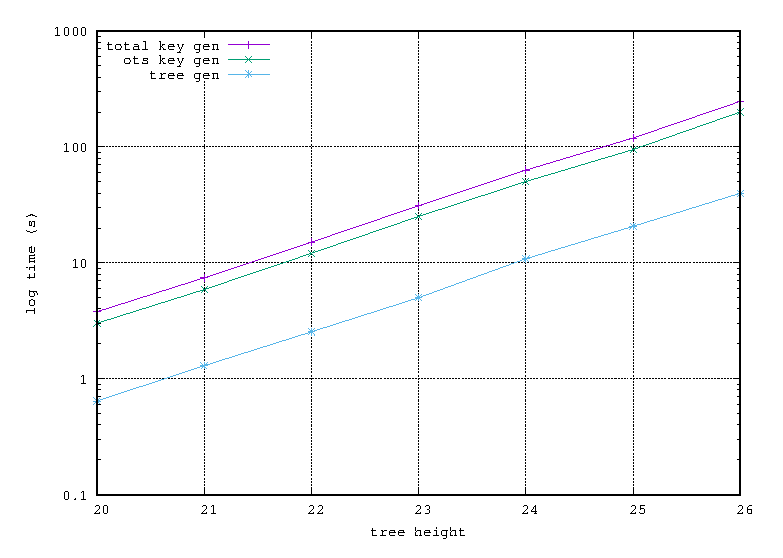
\includegraphics[trim={1mm 0 4mm 0},clip,width=\textwidth]{figures/key_gen.eps}\\
  \caption{Chipmunk key generations time.}
  \end{subfigure}
\begin{subfigure}[b]{0.49\textwidth}    \centering
  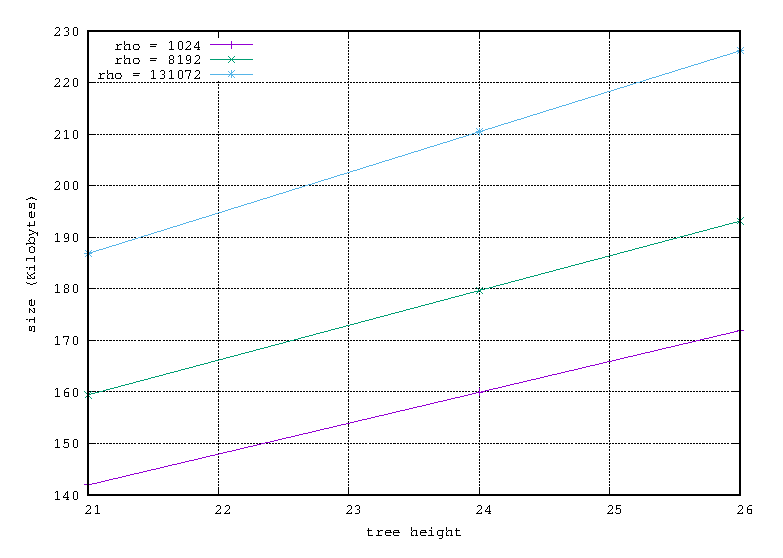
\includegraphics[trim={1mm 0 4mm 0},clip,width=\textwidth]{figures/sig_size.eps}\\
  \caption{Chipmunk aggregated signature size}
  \label{fig:sigize}
  \end{subfigure}
  \caption{Plots showing the scaling characteristics of the key generation time and aggregated signature size of Chipmunk.} \label{fig:keygen}
\end{figure}

\subsubsection{One Aggregate Signature under the Microscope.}

%\mbox{}\gnote{@Zhenfei: Needs rewriting and updating the actual numbers once optimization was run. Please check that it's correct for the camera-ready version}.

To better understand the size of Chipmunk aggregate signatures, we also inspected the sizes of the aggregate signature's individual components.
For the sake of concreteness, let us just consider $\tau=21$ and $\rho=1024$.
An aggregated signature of size approx $118$ Kilobytes,
fitting inside a single ethereum block whose peak size is around 130 Kilobytes\footnote{\url{https://etherscan.io/chart/blocksize}}.
It consists of the following three components.

First, an encoding of the aggregated path and its adjacent nodes. %, as well as the aggregated decomposed public keys.
The aggregated path and its adjacent nodes belong to the homomorphic vector commitment, i.e. $2\tau\limbs$ polynomials in $\ring$ with an infinity norm bound $\bagg$.
We use the encoding method to encode half of those ring elements. Therefore, all these nodes can be represented with $\tau\limbs$ polynomials bounded by $\beta_{\texttt{encode}}$; 
and another $\tau\limbs$ polynomials bounded by $\bagg$. The total size of the path is $\tau\limbs n((\log(\beta_{\texttt{encode}})+1) + (\log(\bagg)+1)) = 102$ Kilobytes.

The aggregated decomposed public keys for the one time signature scheme, i.e., $2\limbs'$ polynomials in $\ring$ with a same norm bound $\bagg$. This requires $2\limbs'n(\log(\bagg)+1)=8$ Kilobytes.

The last component is the aggregated one time signature, i.e., $\otspkkeylen$ polynomials in $\ring$ with norm bound $\beta_\sigma < 2^{20}$, that constitutes $\otspkkeylen n (\log(\beta_\sigma)+1)=8$ Kilobytes. %\gnote{@Zhenfei/Mark:Grammar}

The total size of the aggregated signature is therefore $102 + 8 + 8 = 118$ Kilobytes.




%% Bibliography
\bibliographystyle{alpha}
\bibliography{../cryptobib/abbrev0,../cryptobib/crypto,../extraref}
%\newpage
%\section*{Supplementary Material}
%\input{sections/appendix}
\begin{appendix}
  % !TEX root = ../main.tex
%%% NOTE: I changed notations. Be sure that gamma is the correct thing.

% \begin{table}
% \centering
% \begin{tabular}{@{\makebox[3em][r]{\rownumber\space}} l@{\hspace{3em}}rl}
% \toprule
%  \multicolumn{1}{@{\makebox[3em][r]{\#\space}} c}{Source}&\multicolumn{2}{c}{Constraint}\\
% \midrule
%  \autoref{lem:kots_correct}& $\beta_\sigma \geq$&$ 4\varphi\alpha_H\sqrt{\tfrac{1}{2}\alpha_w\rho(\varepsilon+1+\log_2n\gamma)\cdot\ln2}$\\
%  \autoref{lem:keyhidden}& $\gamma\geq$&$((3\secpar+\delta)/n+\log_2q)\log^{-1}_2(\varphi+\tfrac{1}{2})$\\
%  \autoref{lem:keyhidden}& $\abs{\tern_{\alpha_H}} \leq$&$ 2^{2\secpar + \delta}$\\
%  \autoref{lem:nilssupportivechildsupport}&$q>$&$ 16 \alpha_w \alpha_H\varphi$\\
%  \autoref{lem:kots_sis}&$\abs{\tern_{\alpha_H}} \geq$&$ 2^{2\secpar}$\\
%  \autoref{lem:hvcprobhom}&$\bagg \geq$&$ \eta\sqrt{2\alpha_w\rho(\epsilon + 1 + \log_2 n + \log_2(2\tau \lceil\log_{2\eta+1}q\rceil + \xi\lceil\log_{2\eta+1}q'\rceil))\cdot\ln2}$
% %\bottomrule
% \end{tabular}
% \caption{The constraints a set of Chipmunk parameters needs to satisfy.}\label{tab:constraints}
% \end{table}
\section{Concrete Parameters}\label{sec:concreteparams}

We used a script\footnote{
\url{https://github.com/GottfriedHerold/Chipmunk}%label removed -- Gotti, was causes errors due to multiple-defined label
}
to find concrete parameters that allow for instantiating Chipmunk based on a hard ring-SIS problem.
We have used a fixed ring dimension $n = 512$.
A selection of possible parameter choices is given in Table~\ref{tab:param}.

% ┌──────────┬───────┬────────┬───────────┬───────────┬───────┬───────────┬───────┬─────────┬──────────────┬──────────┬───────┬────────────┬──────────┬────────┐
% &   secpar &   tau &    rho & epsilon   &   alpha_w &   chi &   alpha_H &   phi &   gamma &   beta_sigma &       q' &   eta &   beta_agg &        q & size   &
% ├──────────┼───────┼────────┼───────────┼───────────┼───────┼───────────┼───────┼─────────┼──────────────┼──────────┼───────┼────────────┼──────────┼────────┤
% &      112 &    21 &   1024  &        16 &    12 &        37 &    13 &       6 &       761464 &  3115009 &    73 &      62279 &   514049 & 92 KB  &
% &      112 &    21 &   8192  &        16 &    12 &        37 &    16 &       6 &      2650762 & 10684417 &   110 &     265431 &  2123777 & 109 KB &
% &      112 &    21 & 131072  &        16 &    12 &        37 &    13 &       7 &      8649632 & 34676737 &   163 &    1573282 & 12587009 & 128 KB &
% &      112 &    23 &   1024  &        16 &    12 &        37 &    13 &       6 &       761464 &  3115009 &    73 &      62401 &   514049 & 99 KB  &
% &      112 &    23 &   8192  &        16 &    12 &        37 &    16 &       6 &      2650762 & 10684417 &   110 &     265951 &  2148353 & 118 KB &
% &      112 &    23 & 131072  &        16 &    12 &        37 &    13 &       7 &      8649632 & 34676737 &   163 &    1576360 & 12623873 & 138 KB &
% &      112 &    24 &   1024  &        16 &    12 &        37 &    13 &       6 &       761464 &  3115009 &    73 &      62458 &   514049 & 103 KB &
% &      112 &    24 &   8192  &        16 &    12 &        37 &    16 &       6 &      2650762 & 10684417 &   110 &     266194 &  2148353 & 123 KB &
% &      112 &    24 & 131072  &        16 &    12 &        37 &    13 &       7 &      8649632 & 34676737 &   163 &    1577802 & 12623873 & 144 KB &
% &      112 &    26 &   1024  &        16 &    12 &        37 &    13 &       6 &       761464 &  3115009 &    73 &      62565 &   514049 & 110 KB &
% &      112 &    26 &   8192  &        16 &    12 &        37 &    16 &       6 &      2650762 & 10684417 &   110 &     266652 &  2148353 & 132 KB &
% &      112 &    26 & 131072  &        16 &    12 &        37 &    13 &       7 &      8649632 & 34676737 &   163 &    1580518 & 12644353 & 154 KB &
% &      128 &    21 &   1024  &        19 &    14 &        44 &     9 &       7 &       685898 &  2836481 &    71 &      66007 &   534529 & 93 KB  &
% &      128 &    21 &   8192  &        19 &    14 &        44 &     8 &       8 &      1730419 &  7026689 &    26 &      68809 &   557057 & 144 KB &
% &      128 &    21 & 131072  &        19 &    14 &        44 &     9 &       8 &      7786884 & 31221761 &    37 &     391681 &  3168257 & 167 KB &
% &      128 &    23 &   1024  &        19 &    14 &        44 &     9 &       7 &       685898 &  2836481 &    71 &      66136 &   534529 & 100 KB &
% &      128 &    23 &   8192  &        19 &    14 &        44 &     8 &       8 &      1730419 &  7026689 &    26 &      68942 &   557057 & 156 KB &
% &      128 &    23 & 131072  &        19 &    14 &        44 &     9 &       8 &      7786884 & 31221761 &    37 &     392437 &  3168257 & 181 KB &
% &      128 &    24 &   1024  &        19 &    14 &        44 &     9 &       7 &       685898 &  2836481 &    71 &      66197 &   534529 & 104 KB &
% &      128 &    24 &   8192  &        19 &    14 &        44 &     8 &       8 &      1730419 &  7026689 &    26 &      69004 &   557057 & 162 KB &
% &      128 &    24 & 131072  &        19 &    14 &        44 &     9 &       8 &      7786884 & 31221761 &    37 &     392792 &  3168257 & 188 KB &
% &      128 &    26 &   1024  &        19 &    14 &        44 &     9 &       7 &       685898 &  2836481 &    71 &      66311 &   534529 & 112 KB &
% &      128 &    26 &   8192  &        19 &    14 &        44 &     8 &       8 &      1730419 &  7026689 &    26 &      69122 &   557057 & 174 KB &
% &      128 &    26 & 131072  &        19 &    14 &        44 &     9 &       8 &      7786884 & 31221761 &    37 &     393459 &  3168257 & 202 KB &
% └──────────┴───────┴────────┴───────────┴───────────┴───────┴───────────┴───────┴─────────┴──────────────┴──────────┴───────┴────────────┴──────────┴────────┘

\bgroup
\setlength{\tabcolsep}{0.5em}
\renewcommand{\arraystretch}{1.05}
\begin{table}\centering
    \begin{tabular}{ccr|cc|cccrr|crr|c}%\hline
  
      \multicolumn{3}{c|}{Parameter Sets}
      & \multicolumn{2}{c|}{}
      & \multicolumn{5}{c|}{KOTS Parameters}  
      & \multicolumn{3}{c|}{HVC Parameters}  
      &  {\bf Agg. Sig. Size}\\%\cline{1-3}\cline{5-9}\cline{10-12}
      
      $\lambda$      & $\tau$
      & \multicolumn{1}{c|}{$\rho$}& $\alpha_w$ & $\chi$  &$\alpha_H$& $\varphi$ 
      & $\gamma$                      & \multicolumn{1}{c}{$\beta_\sigma$}     
      & \multicolumn{1}{c|}{$q'$}                     & $\eta$       
      & $\bagg\quad$                  & \multicolumn{1}{c|}{$q$} 
      & (Kilobytes) \\\toprule
  
  
      % &       &        &            &  &  \multicolumn{4}{c||}{HVC}  &  & \multicolumn{2}{c||}{KOTS}  & (Kilobytes) \\\hline\hline

          &       &   1024  &        16 &    12 &        37 &    13 &       6 &        761,464 &  3,115,009 &    73 &       62,279 &    514,049 & 92 KB  \\
          &    21 &   8192  &        16 &    12 &        37 &    16 &       6 &      2,650,762 & 10,684,417 &   110 &      265,431 &  2,123,777 & 109 KB \\
          &       & 131072  &        16 &    12 &        37 &    13 &       7 &      8,649,632 & 34,676,737 &   163 &    1,573,282 & 12,587,009 & 128 KB \\\cline{2-14}

          &       &   1024  &        16 &    12 &        37 &    13 &       6 &        761,464 &  3,115,009 &    73 &       62,458 &    514,049 & 103 KB \\
      112 &    24 &   8192  &        16 &    12 &        37 &    16 &       6 &      2,650,762 & 10,684,417 &   110 &      266,194 &  2,148,353 & 123 KB \\
          &       & 131072  &        16 &    12 &        37 &    13 &       7 &      8,649,632 & 34,676,737 &   163 &    1,577,802 & 12,623,873 & 144 KB \\\cline{2-14}

          &       &   1024  &        16 &    12 &        37 &    13 &       6 &        761,464 &  3,115,009 &    73 &       62,565 &    514,049 & 110 KB \\
          &    26 &   8192  &        16 &    12 &        37 &    16 &       6 &      2,650,762 & 10,684,417 &   110 &      266,652 &  2,148,353 & 132 KB \\
          &       & 131072  &        16 &    12 &        37 &    13 &       7 &      8,649,632 & 34,676,737 &   163 &    1,580,518 & 12,644,353 & 154 KB \\\midrule

          &       &   1024  &        19 &    14 &        44 &     9 &       7 &        685,898 &  2,836,481 &    71 &       66,007 &    534,529 & 93 KB  \\
          &    21 &   8192  &        19 &    14 &        44 &     8 &       8 &      1,730,419 &  7,026,689 &    26 &       68,809 &    557,057 & 144 KB \\
          &       & 131072  &        19 &    14 &        44 &     9 &       8 &      7,786,884 & 31,221,761 &    37 &      391,681 &  3,168,257 & 167 KB \\\cline{2-14}

          &       &   1024  &        19 &    14 &        44 &     9 &       7 &        685,898 &  2,836,481 &    71 &       66,197 &    534,529 & 104 KB \\
      128 &    24 &   8192  &        19 &    14 &        44 &     8 &       8 &      1,730,419 &  7,026,689 &    26 &       69,004 &    557,057 & 162 KB \\
          &       & 131072  &        19 &    14 &        44 &     9 &       8 &      7,786,884 & 31,221,761 &    37 &      392,792 &  3,168,257 & 188 KB \\\cline{2-14}

          &       &   1024  &        19 &    14 &        44 &     9 &       7 &        685,898 &  2,836,481 &    71 &       66,311 &    534,529 & 112 KB \\
          &    26 &   8192  &        19 &    14 &        44 &     8 &       8 &      1,730,419 &  7,026,689 &    26 &       69,122 &    557,057 & 174 KB \\
          &       & 131072  &        19 &    14 &        44 &     9 &       8 &      7,786,884 & 31,221,761 &    37 &      393,459 &  3,168,257 & 202 KB \\\bottomrule

  %     &       &   1024 &         16 &        12 &        37 &         13 &       6 &        761464 &  3115009 &    73 &       62279 &   202,753 & 120 \\%\cline{3-13}
  %     &    21 &   8192 &         16 &        12 &        37 &         16 &       6 &      2650762 & 10684417 &    110 &      265431 &   962,561 & 135 \\%\cline{3-13}
  %     &       & 131072 &         16 &        12 &        37 &         13 &       7 &      8649632 & 34676737 &    163 &      1573282 & 7,790,593 & 158 \\\cline{2-14}
  
  %     &       &   1024 &         16 &        12 &        37 &         13 &       6 &        761464 &  3115009 &    73 &       62458 &   202,753 & 135 \\%\cline{3-13}
  % 112 &    24 &   8192 &         16 &        12 &        37 &         16 &       6 &      2650762 & 10684417 &    110 &      266194 &   964,609 & 152 \\%\cline{3-13}
  %     &       & 131072 &         16 &        12 &        37 &         13 &       7 &      8649632 & 34676737 &    163 &     1577802 & 7,790,593 & 178 \\\cline{2-14}
  
  %     &       &   1024 &         16 &        12 &        37 &         13 &       6 &        761464 &  3115009 &    73 &       62565 &   202,753 & 145 \\%\cline{3-13}
  %     &    26 &   8192 &         16 &        12 &        37 &         16 &       6 &      2650762 & 10684417 &    110 &      266652 &   995,329 & 163 \\%\cline{3-13}
  %     &       & 131072 &         16 &        12 &        37 &         13 &       7 &      8649632 & 34676737 &    163 &     1580518 & 7,806,977 & 191 \\\midrule
  
  %     &       &   1024 &         19 &        14 &        44 &          9 &       7 &        685898 &  2836481 &    71 &      66007 &   249,857 & 121 \\%\cline{3-13}
  %     &    21 &   8192 &         19 &        14 &       44 &          8 &       8 &      1730419 &  7026689 &    26 &       68809 &   270,337 & 167 \\%\cline{3-13}
  %     &       & 131072 &         19 &        14 &       44 &          9 &       8 &      7786884 & 31221761 &    37 &     391681 & 1,492,993 & 197 \\\cline{2-14}
  
  %     &       &   1024 &         19 &        14 &       44 &          9 &       7 &        685898 &  2836481 &    71 &       66197 &   249,857 & 136 \\%\cline{3-13}
  % 128 &    24 &   8192 &         19 &        14 &       44 &          8 &       8 &      1730419 &  7026689 &    26 &       69004 &   270,337 & 188 \\%\cline{3-13}
  %     &       & 131072 &         19 &        14 &       44 &          9 &       8 &      7786884 & 31221761 &    37 &      392792 & 1,492,993 & 222 \\\cline{2-14}
  
  %     &       &   1024 &         19 &        14 &       44 &          9 &       7 &        685898 &  2836481 &    71 &       66311 &   249,857 & 146 \\%\cline{3-13}
  %     &    26 &   8192 &         19 &        14 &       44 &          8 &       8 &      1730419 &  7026689 &    26 &       69122 &   270,337 & 202 \\%\cline{3-13}
  %     &       & 131072 &         19 &        14 &       44 &          9 &       8 &      7786884 & 31221761 &    37 &     3934594 & 1,492,993 & 239 \\\bottomrule
    \end{tabular}
    \caption{Parameter sets for Chipmunk for a fixed ring dimension $n=512$.}\label{tab:param}
  \end{table}
\egroup


  \section{Proof of \autoref{theo:kots}}\label{app:proofs}
\begin{proof}
The theorem follows from \autoref{lem:kots_ind_correct}, \autoref{lem:kots_correct}, \autoref{lem:kots_homomorphic}, and \autoref{lem:kots_sis}.
\end{proof}

The following four lemmas state that our construction satisfies the desired homomorphic properties and that it is unforgeable.
\begin{lemma}\label{lem:kots_ind_correct}
Let $\secpar, \varepsilon, \alpha_w$, $\alpha_H$, $\varphi$, $\gamma$, $\rho$, $\beta_\sigma,n,q$ be positive integers, such that $n$ is a power of two, $q$ is prime.
  Let $\ring_q$ be the polynomial ring $\ZZ_q[x]/\langle x^n+1\rangle$.
Let $H : \bin^* \to \tern_{\alpha_H}$ be a hash function.
  Then the construction from \autoref{fig:otsconstruction} is a individually correct one time signature scheme.
\end{lemma}
\begin{proof}
  Let $\params \gets \setup(\secparam)$, $(\osk,\opk) \gets \kgen(\params)$, $m\in\bin^*$ and $\vec{\sigma} \gets \sign(\params,\osk,m)$ be arbitrary.
  We first observe that the check on the \emph{value} of the signature goes through, as
  \begin{align*}
    \vec{a}^\intercal\vec{\sigma}
    ={}&\vec{a}^\intercal(\vec{s}_0\cdot H(m) + \vec{s}_1)\tag{Def. of $\sign$}\\
    ={}&\vec{a}^\intercal\vec{s}_0\cdot H(m) + \vec{a}^\intercal\vec{s}_1 \tag{Distributivity}\\
    ={}&v_0\cdot H(m) + v_1. \tag{Def. of $\kgen$}
  \end{align*}
  The signature also does not violate the norm bound, as
  \begin{align*}
    \norm{\vec{\sigma}}
    ={}&\norm{\vec{s}_0\cdot H(m) + \vec{s}_1} \tag{Def. of $\sign$}\\
    \leq{}&\norm{\vec{s}_0\cdot H(m)} + \norm{\vec{s}_1}\\
    \leq{}&\norm{\vec{s}_0}\cdot\norm{H(m)}_1 + \norm{\vec{s}_1} \tag{\autoref{lem:ternbound}}\\
    ={}&2\varphi\alpha_H \tag{Def. of $\kgen$}.
  \end{align*}
  The lemma thus follows.
\end{proof}


\begin{lemma}\label{lem:kots_correct}
Let $\secpar, \varepsilon, \alpha_w$, $\alpha_H$, $\varphi$, $\gamma$, $\rho$, $\beta_\sigma$, $n$, $q$ be positive integers, such that \[\beta_\sigma \geq 4\varphi\alpha_H\sqrt{\tfrac{1}{2}\alpha_w\rho(\varepsilon+1+\log_2n\gamma)\cdot\ln2}.\]
  Let $\ring_q$ be the polynomial ring $\ZZ_q[x]/\langle x^n+1\rangle$.
  Let $H : \bin^* \to \tern_{\alpha_H}$ be a hash function.
  Then the construction from \autoref{fig:otsconstruction} is a $(\rho,\tern_{\alpha_w},\varepsilon)$-probabilistically homomorphic one time signature scheme.
\end{lemma}

\begin{proof}
  Let $\ell\in[\rho]$, $m\in\bin^*$, and $\params\gets\setup(\secparam)$ and for $i\in[\ell]$ let $\opk^i=(v_0,v_1) \in \ring_q^2$ and $\vec{\sigma}^i \in \ring_q^\gamma$ be arbitrary such that for all $i\in[\ell]$, $\iverify(\params,\opk^i,m,\vec{\sigma}^i)=1$.
  
  We first note that even for arbitrary $w_1,\dots,w_\ell \in \tern_\alpha$ it holds that
  \begin{align*}
    \vec{a}^\intercal\cdot \sum_{i=1}^{\ell-1}w^i\cdot\vec{\sigma}^i
    ={}&\sum_{i=1}^{\ell}w^i\cdot\vec{a}^\intercal\vec{\sigma}^i \tag{Distributivity}\\
    ={}&\sum_{i=1}^{\ell}w^i\cdot(v^i_0\cdot H(m)+v^i_1) \tag{Def. of $\iverify$}\\
%    ={}&\sum_{i=1}^{\ell}w^iv^i_0\cdot H(m)+ \sum_{i=1}^{\ell}w^iv^i_1 \tag{Distributivity}\\
    ={}&\Bigl(\sum_{i=1}^{\ell}w^iv^i_0\Bigr)\cdot H(m)+ \Bigl(\sum_{i=1}^{\ell}w^iv^i_1\Bigr) \tag{Distributivity}.
  \end{align*}
  
  Therefore, it only remains to verify that the norm-check goes through with sufficient probability.
  I.e., that
  \[
    \Pr\mleft[
      w^1,\dots,w^\ell\gets \tern_{\alpha_w}
      :
      \Bigl\Vert\sum_{i=1}^{\ell} w^i\cdot\vec{\sigma}^i\Bigr\Vert \leq \beta_\sigma\mright] \leq 2^{-\varepsilon}.
  \]
  To bound this probability, consider that the norm-bound is violated iff the absolute value of at least one of the $n\gamma$ coefficients in $\sum_{i=1}^{\ell} w^i\cdot\vec{\sigma}^i$ is greater than $\beta_\sigma$.
  By a union bound it is thus sufficient to show that each individual coefficient violates the bound with probability at most $2^{-\varepsilon}/(n\gamma)$
  
  For each individual $\vec{\sigma}^i$ it holds by the definition of $\iverify$ that
    $\norm{\vec{\sigma}^i} \leq 2\varphi\alpha_H$
  Therefore, each coefficient is a sum of the form
  \(
    \sum_{j=1}^{\alpha_w\ell}b_j c_j
  \)
  where $\abs{c_j}\leq 2\varphi\alpha_H$ and $b_j$ is chosen uniformly from $\{-1,1\}$.
  By linearity of expectation, the expected value of this sum is always zero and changing any summand can vary the sum by at most $4\varphi\alpha_H$. We can thus apply McDiarmid's inequality~\cite{McDiarmid89} and the lower bound on $\beta_\sigma$ from the lemma statement to obtain the following bound on the probability that each individual coefficient exceeds the norm bound $\beta_\sigma$:
  \begin{align*}
    &\Pr\Bigl[\vec{b}\gets\{-1,1\}^{\alpha_w\ell} : \Bigl|\smashoperator{\sum_{j=1}^{\alpha_w\ell}}b_j c_j\Bigr| > \beta_\sigma\Bigr]\\
    \leq{}& 2\cdot\exp\Bigl(-\frac{2\beta_\sigma^2}{\alpha_w\ell\cdot (4\varphi\alpha_H)^2}\Bigr)\\
    \leq{}& 2\cdot\exp\Bigl(-\frac{2\beta_\sigma^2}{\alpha_w\rho\cdot (4\varphi\alpha_H)^2}\Bigr)\\
    \leq{}& 2\cdot\exp\Bigl(-\frac{2(4\varphi\alpha_H)^2\cdot\tfrac{1}{2}\alpha_w\rho(\varepsilon+1+\log_2n\gamma)\cdot\ln2}{\alpha_w\rho\cdot (4\varphi\alpha_H)^2}\Bigr)\\
    ={}& 2\cdot\exp(-(\varepsilon+1+\log_2n\gamma)\cdot\ln2)\\
    ={}& 2^{-\varepsilon-\log_2n\gamma} = 2^{-\varepsilon}\cdot \frac{1}{n\gamma}
  \end{align*}
  It thus follows that with probability at least $1-2^\varepsilon$ the strong verification algorithm outputs $1$ as required.
\end{proof}


\begin{lemma}\label{lem:kots_homomorphic}
  Let $\secpar, \alpha_H$, $\varphi$, $\gamma$, $\beta_\sigma,q,n,\secpar$ be positive integers.
  Let $\ring_q$ be the polynomial ring $\ZZ_q[x]/\langle x^n+1\rangle$.
  Let $H : \bin^* \to \tern_{\alpha_H}$ be a hash function.
  Then the construction from \autoref{fig:otsconstruction} is a robustly homomorphic.
\end{lemma}

\begin{proof}
  Let $\params\gets\setup(\secparam)$, $m\in\bin^*$, $\opk^0=(v^0_0,v^0_1),\opk^1=(v^1_0,v^1_1)\in \ring^2_q$, and $\vec{\sigma}^0,\vec{\sigma}^1 \in \ring_q^\gamma$ be arbitrary such that \[\sverify(\params,\opk^0,m,\vec{\sigma}^0)=1 \quad\text{and}\quad \sverify(\params,\opk^1,m,\vec{\sigma}^1)=1.\]
  
  By the definition of the strong verification algorithm, it holds that
  \begin{equation*}
     \norm{(\vec{\sigma}^0-\vec{\sigma}^1)}
    \leq \norm{\vec{\sigma}^0}+\norm{\vec{\sigma}^1}
    \leq 2\beta_\sigma,
  \end{equation*}
  thus the norm check goes through.
  It remains to verify that the second check also goes through.
  \begin{align*}
     \vec{a}^\intercal\cdot (\vec{\sigma}^0-\vec{\sigma}^1)
    ={}& \vec{a}^\intercal\cdot \vec{\sigma}^0- \vec{a}^\intercal\cdot\vec{\sigma}^1\\
    ={}& (v^0_0\cdot H(m) + v^0_1) - (v^1_0\cdot H(m) + v^1_1)\tag{Def of $\sverify$}\\
    ={}& (v^0_0-v^1_0)\cdot H(m) + (v^0_1-v^1_1).
  \end{align*}
  Therefore, the lemma statement follows.
\end{proof}


\begin{lemma}\label{lem:kots_sis}
  Let $n,\gamma,q,\alpha_H,\alpha_w,\delta,\secpar$ be positive integers with $q$ prime and $n$ a power of two, such that $q > 16 \alpha_w \alpha_H\varphi$, $\gamma\geq((3\secpar+\delta)/n+\log_2q)\log^{-1}_2(\varphi+\tfrac{1}{2})$, and $2^{2\secpar} \leq \abs{\tern_{\alpha_H}} \leq 2^{2\secpar + \delta}$.
  Let $H : \bin^* \to \tern_{\alpha_H}$ be a hash function.
  If the $\sis_{\ring,q,\gamma,2\beta_\sigma + 4\alpha_w\alpha_H\varphi}$ problem is hard and $H$ is collision resistant, then the construction from \autoref{fig:otsconstruction} is existentially unforgeable under rerandomized keys.
\end{lemma}

\begin{proof}
  Let $\adv$ be an arbitrary adversary against the multi-user $W'$-existentially unforgeability under rerandomized keys with success probability $\nu(\secpar)$.
  We construct an algorithm $\bdv$ that solves $\sis_{\ring,q,\gamma,2\beta_\sigma + 4\alpha_w\alpha_H\varphi}$ as follows.
  Given $\vec{a}\in\ring_q^\gamma$, $\bdv$ honestly chooses secret keys $(\vec{s}^i_0,\vec{s}^i_1) \in \ball_{\varphi}^\gamma\times \ball_{\varphi\alpha_H}^\gamma$ uniformly at random for $i\in[T-1]$ and invokes $\adv$ on public keys $(v^i_0,v^i_1)$, with $v^i_b := \vec{a}^\intercal\cdot s^i_b$.
  Whenever $\adv$ sends a signing query $(i,m)$, $\bdv$ will respond with the honestly computed signature $\vec{\sigma}:=\vec{s}^i_0\cdot H(m)+ \vec{s}^i_1$.
  Eventually $\adv$ outputs a candidate forgery $(i^*,m^*,\vec{\sigma}^*,w^*)$ and $\bdv$ will compute a signature on the same message as $\vec{\sigma}' := w^*\cdot\vec{s}^{i^*}_0\cdot H(m^*)+ w^*\cdot\vec{s}^{i^*}_1$.
  It then outputs $\vec{\sigma}^*-\vec{\sigma}'$.
  
  To analyze the success probability of $\bdv$ suppose that $\adv$ outputs a \emph{valid} forgery.
  I.e., at most a single query was asked for index $i^*$, said query was \emph{not} $m^*$, $w^*\in W'$ and $\wverify(\vec{a},(w^*v^{i^*}_0,w^*v^{i^*}_1),m^*,\allowbreak\vec{\sigma}^*)=1$.
  From this and the definition of $\vec{\sigma}'$ above it follows that
  \begin{align*}
       &\vec{a}^\intercal\cdot(\vec{\sigma}^*-\vec{\sigma}')\\ ={}& \vec{a}^\intercal\vec{\sigma}^*-\vec{a}^\intercal\vec{\sigma}'\\ 
    ={}& (w^*\cdot v^{i^*}_0 H(m) + w^*\cdot v^{i^*}_1) - \vec{a}^\intercal(w^*\cdot \vec{s}^{i^*}_0\cdot H(m^*)+ w^*\cdot\vec{s}^{i^*}_1)\\
    ={}& (w^*\cdot v^{i^*}_0 H(m) + w^*\cdot v^{i^*}_1) - (w^*\cdot\vec{a}^\intercal\vec{s}^{i^*}_0\cdot H(m^*)+ w^*\cdot\vec{a}^\intercal\vec{s}^{i^*}_1)\\
    ={}& (w^*\cdot v^{i^*}_0\cdot H(m) + w^*\cdot v^{i^*}_1) - (w^*\cdot v^{i^*}_0\cdot H(m) + w^*\cdot v^{i^*}_1) = 0.
  \end{align*}
  as required for a solution to the SIS problem.
  
  Next, to argue that $\norm{\vec{\sigma}^*-\vec{\sigma}'}\leq 2\beta_\sigma + 4\alpha_w\alpha_H\varphi$, note that the weak verification algorithm guarantees that $\norm{\vec{\sigma}^*} \leq 2\beta_\sigma$.
  Further, since $w^*\in W'$ there exist $w_0,w_1 \in \tern_{\alpha_w}$ such that $w^* = w_0-w_1$ and $\norm{w^*}_1 \leq \norm{w_0}_1 + \norm{w_1}_1 = 2\alpha_w$.
  We can thus bound the norm of $\vec{\sigma}'$ as
  \begin{align*}
    \norm{\vec{\sigma}'} ={}& \norm{w^*\cdot\vec{s}^{i^*}_0\cdot H(m^*)+ w^*\cdot\vec{s}^{i^*}_1}\tag{Def. of $\sign$}\\
    ={}&\norm{w^*\cdot\vec{s}^{i^*}_0\cdot H(m^*)}+ \norm{w^*\cdot\vec{s}^{i^*}_1}\tag{Triangle Inequality}\\
    ={}&\norm{w^*}_1\cdot\norm{H(m^*)}_1\cdot\norm{\vec{s}^{i^*}_0} + \norm{w^*}_1\cdot\norm{\vec{s}^{i^*}_1}\tag{\autoref{lem:ternbound}}\\
    ={}&4\alpha_w\alpha_H\varphi.\tag{$w^*\in W'$ and $H(m^*)\in\tern_{\alpha_H}$}
  \end{align*}
  It follows that $\norm{\vec{\sigma}^*-\vec{\sigma}'} \leq \norm{\vec{\sigma}^*}+\norm{\vec{\sigma}'} \leq 2\beta_\sigma + 4\alpha_w\alpha_H\varphi$ as required.

  Finally, we need to argue that $\vec{\sigma}^*-\vec{\sigma}'\neq 0$.
  This is the case iff $\vec{\sigma}^* \neq \vec{\sigma}'$.
  It thus suffices to bound the probability, that $\vec{\sigma}^*=\vec{\sigma}'$.

  To this end, we observe by \autoref{lem:keyhidden} that, since $\adv$ has learned at most a single signature under $(v_0^{i^*},v_1^{i^*})$, the corresponding $(\vec{s}_0^{i^*},\vec{s}_1^{i^*})$ remains information-theoretically hidden from $\adv$ among at least 2 possible secret keys.
  Once $\adv$ outputs a valid forgery $(i^*,m^*,\vec{\sigma}^*,w^*)$ the signing key used for the forgery becomes uniquely determined by \autoref{lem:nilssupportivechildsupport} as long as $H(m^*)\neq H(m)$ which is guaranteed with overwhelming probability by the collision resistance of $H$.
  It follows that $\sigma^* \neq \sigma'$ with probability at least $1/2 - \negl$.
  Therefore, the success probability of our reduction $\bdv$ is $(1/2 - \negl) \nu(\secpar)$ and since the SIS problem is assumed to be hard, $\nu(\secpar)$ must therefore be negligible in $\secpar$.
  
\end{proof}

\begin{lemma}\label{lem:keyhidden}
  Let $n,\gamma,q,\alpha_H, \delta, \varphi,\secpar$ be positive integers such that $\gamma\geq((3\secpar+\delta)/n+\log_2q)\log^{-1}_2(\varphi+\tfrac{1}{2})$ and $\abs{\tern_{\alpha_H}} \leq 2^{2\secpar + \delta}$, let $\ring=\ZZ[x]/(x^n+1)$. Then for any $\vec{a}\in\ring_q^\gamma$ and uniformly chosen $(\vec{s}_0,\vec{s}_1)\in \ball_{\varphi}^\gamma \times \ball_{\varphi\alpha_H}^\gamma$ it holds with probability at least $1-2^{-\lambda}$ that for every $c\in \tern_{\alpha_H}$ there exists $(\vec{s}'_0,\vec{s}'_1)\in \ball_{\varphi}^\gamma \times \ball_{\varphi\alpha_H}^\gamma$such that $(\vec{s}'_0,\vec{s}'_1)\neq(\vec{s}_0,\vec{s}_1)$, $(\vec{a}^\intercal\cdot\vec{s}'_0,\vec{a}^\intercal\cdot\vec{s}'_1) = (\vec{a}^\intercal\cdot\vec{s}_0,\vec{a}^\intercal\cdot\vec{s}_1)$ and $\vec{s}'_0\cdot c + \vec{s}'_1 = \vec{s}_0\cdot c + \vec{s}_1$.
\end{lemma}
\begin{proof}
  We define a function $f_{\vec{a}, c}$ that maps any secret key $(\vec{s}_0, \vec{s}_1)$ to a pair of public key and signature defined as $((\vec{a}^\intercal\cdot\vec{s}_0,\vec{a}^\intercal\cdot\vec{s}_1), \vec{s}_0\cdot c + \vec{s}_1)$.
  We will show that the domain of this function is at least $2^{3\secpar + \delta}$ times larger than the range.
  The number of possible secret keys is $(2\varphi+1)^{n\gamma} \cdot (2\varphi\alpha_H+1)^{n\gamma}$.
  The number of possible signatures is at most $(4\varphi\alpha_H + 1)^{n\gamma}$.
  For fixed values $\vec{a}, c, \vec{s}_0\cdot c + \vec{s}_1$, we observe that once $\vec{a}^\intercal\cdot\vec{s}_0$ is fixed, the second component $\vec{a}^\intercal\cdot\vec{s}_1 = \vec{a}^\intercal \cdot ((\vec{s}_0\cdot c + \vec{s}_1) - \vec{s}_0 \cdot c)$ is uniquely determined.
  Thus for a fixed signature, there are at most $q^n$ many possible public keys and therefore the size of the range of $f_{\vec{a}, c}$ is at most $(4 \varphi\alpha_H + 1)^{n\gamma} \cdot q^n$.
  We observe that
  \begin{align*}\frac{(2\varphi+1)^{n\gamma} \cdot (2\varphi\alpha_H+1)^{n\gamma}}{(4 \varphi\alpha_H + 1)^{n\gamma} \cdot q^n}
   \geq{}& \frac{(2\varphi+1)^{n\gamma} \cdot (2\varphi\alpha_H+1)^{n\gamma}}{(4 \varphi\alpha_H + 2)^{n\gamma} \cdot q^n}\\
   ={}& \frac{(2\varphi+1)^{n\gamma}}{2^{n\gamma} \cdot q^n}\\
   ={}& (\varphi+\frac{1}{2})^{n\gamma} \cdot q^{-n}\\
   ={}& 2^{\log_2(\varphi+\frac{1}{2})\cdot{n\gamma} - n \log_2 q}
  \end{align*}
  Using the condition on $\gamma$ from the lemma statement, one can see that
  \[
    \log_2(\varphi+\frac{1}{2})\cdot{n\gamma} - n \log_2 q
    \geq n\Bigl(\frac{3\secpar+\delta}{n}+\log_2q\Bigr) - n \log_2 q = 3\secpar+\delta
  \]
  and thus, as claimed the domain of $f_{\vec{a},c}$ is at least $2^{3\secpar + \delta}$ times larger than its range.
  
  Using Lemma 4.1 from~\cite{TCC:LyuMic08}, the probability, over a uniformly chosen secret key, that there exists $(\vec{s}'_0,\vec{s}'_1)\in \ball_{1}^\gamma \times \ball_{\beta_s}^\gamma$ such that $(\vec{s}'_0,\vec{s}'_1)\neq(\vec{s}_0,\vec{s}_1)$, $(\vec{a}^\intercal\cdot\vec{s}'_0,\vec{a}^\intercal\cdot\vec{s}'_1) = (\vec{a}^\intercal\cdot\vec{s}_0,\vec{a}^\intercal\cdot\vec{s}_1)$ and $\vec{s}'_0\cdot c + \vec{s}'_1 = \vec{s}_0\cdot c + \vec{s}_1$ is at least $1-2^{-3\secpar-\delta}$.
  By union bounding over all possible hash values $c \in \tern_{\alpha_H}$ and observing that $\tern_{\alpha_H} \leq 2^{2\secpar + \delta}$ the lemma statement follows. 
\end{proof}

\begin{lemma}\label{lem:nilssupportivechildsupport}
Let $n,\gamma,q,\alpha_H, \alpha_w$ be positive integers with $q$ prime and $n$ a power of two such that $q > 16 \alpha_w \alpha_H\varphi$ and let $\ring=\ZZ[x]/(x^n+1)$. Let $\vec{a}\in\ring_q^\gamma$, $c_0,c_1 \in \tern_{\alpha_{H}}$, $w_0, w_1 \in \tern_{\alpha_w}$, and $\sigma_0,\sigma_1 \in \ring$ be arbitrary ring elements such that $c_0\neq c_1$ and $w_0 \neq w_1$. Then there exists at most a single pair of vectors $(\vec{s}_0,\vec{s}_1)\in\ball^\gamma_{\varphi}\times \ball^\gamma_{\varphi\alpha_H}$, such that
    \[\vec{s}_0\cdot c_0 + \vec{s}_1 = \sigma_0 \quad\text{and}\quad (w_0 - w_1) \cdot (\vec{s}_0\cdot c_1 + \vec{s}_1) = \sigma_1.\]
\end{lemma}
 \begin{proof}
    Let $(\vec{s}_0, \vec{s}_1)\in\ball^\gamma_{\varphi}\times \ball^\gamma_{\varphi\alpha_H}$ and $(\vec{s}'_0, \vec{s}'_1)\in\ball^\gamma_{\varphi}\times \ball^\gamma_{\varphi\alpha_H}$ be two secret keys, such that 
    \begin{equation}
    \vec{s}_0\cdot c_0 + \vec{s}_1 = \vec{s}'_0\cdot c_0 + \vec{s}'_1 \implies (\vec{s}_0 - \vec{s}'_0)\cdot c_0 + (\vec{s}_1 - \vec{s}'_1) = 0 \label{hello}
    \end{equation}
    and 
    \begin{equation}
    \begin{aligned}
    &(w_0 - w_1) \cdot (\vec{s}_0\cdot c_1 + \vec{s}_1) = (w_0 - w_1) \cdot (\vec{s}'_0\cdot c_1 + \vec{s}'_1)\\ \implies& (w_0 - w_1)((\vec{s}_0 - \vec{s}'_0)\cdot c_1 + (\vec{s}_1 - \vec{s}'_1)) = 0 \label{kitty}
    \end{aligned}
    \end{equation}
    Equation~\ref{hello} implies that 
    \[
    (w_0 - w_1)((\vec{s}_0 - \vec{s}'_0)\cdot c_0 + (\vec{s}_1 - \vec{s}'_1)) = 0.
    \]
    Combined with Equation~\ref{kitty}, we get that in $\ring_q$
    \begin{equation}
    (w_0 - w_1)(\vec{s}_0 - \vec{s}'_0) (c_0 - c_1)  = 0 \label{herekittykitty}
    \end{equation}
    Since $w_0,w_1\in\tern_{\alpha_w}$, $\vec{s}_0,\vec{s}'_0 \in \ball^\gamma_{\varphi}$, and $c_0,c_1\in\tern_{\alpha_{H}}$, it holds by \autoref{lem:ternbound} that
    \[
      \begin{aligned}
      &\norm{(w_0 - w_1)(\vec{s}_0 - \vec{s}'_0) (c_0 - c_1)}\\
       \leq& \norm{w_0 - w_1}_1\cdot\norm{c_0 - c_1}_1\cdot \norm{(\vec{s}_0 - \vec{s}'_0)}\\ \leq& 8\alpha_w\alpha_H\varphi \leq \frac{q-1}{2}.
      \end{aligned}
    \]
    Therefore \autoref{herekittykitty} also holds in $\ring$.
    Since $w_0 \neq w_1$, $c_0 \neq c_1$, and $\ring$ is an integral domain, it follows that $\vec{s}_0 = \vec{s}'_0$.
    By Equation~\ref{hello}, it must therefore hold that $(\vec{s}_0, \vec{s}_1) = (\vec{s}'_0, \vec{s}'_1)$.
    
\end{proof}

\end{appendix}
\end{document}



